\documentclass[ALICE,manyauthors]{cernphprep}
\usepackage[modulo]{lineno}
\usepackage{hyperref}
\usepackage[comma,square,numbers,sort&compress]{natbib}
\usepackage{amsmath,amssymb}% for advanced math typesetting 
\usepackage{url,color}
%\usepackage{pslatex}
\usepackage{mathrsfs} % produce the curly R with \mathscr not \mathcal

% \usepackage{palatino}%    Choose default roman font.  Others are times, pslatex, newcent, bookman, chancery                                                    
% can use mathpazo if no one uses \mathrm{\gamma}, etc., since it doesn't suppl\y Greek in rm. Google "mathpazo mathrm greek"                                   
% \usepackage{mathpazo}%  Matching math fonts (see http://www.math.uiuc.edu/~hartke/computer/latex/survey/survey.html)                                           
% \usepackage{helvet}%

\linenumbers

\newcommand{\tn}[1]{\textnormal{#1}}
\newcommand{\eq}[2]{\begin{equation}\label{#1} #2 \end{equation}}
\newcommand{\eqa}[2]{\begin{align}\label{#1} #2 \end{align}}
\newcommand{\braces}[1]{\left ( #1 \right )}
\newcommand{\typew}[1]{\texttt{#1}}
\newcommand{\abs}[1]{\left| #1 \right|}
\newcommand{\median}[1]{\tn{median}\left\{ #1 \right\}}
\newcommand{\mean}[1]{\tn{mean}\left\{ #1 \right\}}
%Common units
\newcommand{\cm}[0]{\tn{ cm}}
\newcommand{\TeV}[0]{\tn{ TeV}}
\newcommand{\GeV}[0]{\tn{ GeV}}

\newcommand{\aliroot}[0]{\typew{aliroot}}

\usepackage{float}
%\usepackage[pdftex]{hyperref}

\begin{document}
%%%%%%%%%%%%% ptdr definitions %%%%%%%%%%%%%%%%%%%%%
%
%%%%%%%%%%%%%%%  Title page %%%%%%%%%%%%%%%%%%%%%%%%
%

\newcommand{\PbPb}{\textnormal{Pb--Pb}}
\newcommand{\AuAu}{\textnormal{Au--Au}}
\newcommand{\pp}{\ensuremath{\mbox{p}\mbox{p}}}
\newcommand{\snn}{\ensuremath{\sqrt{s_\tn{NN}}}}
\newcommand{\pt}{\ensuremath{p_\tn{T}}}\newcommand{\pT}{\pt}
 % off by redefinding CKBNOTEje
\newcommand{\CKBNOTE}[1]{{\bf CKB:  #1}} 
\renewcommand{\CKBNOTE}[1]{}  % switch off

 % off by redefinding RHNOTE
\newcommand{\RHNOTE}[1]{{\bf RH:  #1}} 
\renewcommand{\RHNOTE}[1]{}  % switch off

\begin{titlepage}
%
\PHyear{2016}
\PHnumber{040}                 % required, obtained from PH
\PHdate{24 Novermer}              % required, will be obtained from PH
%
%
%%% Put your own title + short title here:
\title{Systematic studies of correlations between different order flow harmonics in $\PbPb$ collisions at $\mathbf{\sqrt{s_\mathrm{NN}} = 2.76}$~TeV}
\ShortTitle{Correlations between event-by-event fluctuations of flow harmonics}   % appears on right page headers

%
%%% Do not change the nexts!
\Collaboration{ALICE Collaboration%
         \thanks{See Appendix~\ref{app:collab} for the list of collaboration
                      members}}
\ShortAuthor{ALICE Collaboration}      % appears on left page headers, do not change
%
\begin{abstract}

The correlations between event-by-event fluctuations of amplitudes of anisotropic flow harmonics
in $\PbPb$ collisions at $\snn=2.76$~TeV have been measured with the ALICE detector at the Large Hadron Collider. 
The results were obtained with the new multi-particle cumulant method dubbed symmetric cumulants.
This method is robust against systematic biases originating from non-flow effects. 
The centrality dependence of correlation between the higher harmonics ($v_3$, $v_4$, $v_5$) and the lower harmonics ($v_2$, $v_3$) as well as the transverse momentum dependence of $v_3$-$v_2$ and $v_4$-$v_2$ correlations are presented. 
The results are compared to calculations from viscous hydrodynamics and  A Multi-Phase Transport ({AMPT}) models.
The comparisons to viscous hydrodynamic models demonstrate that
the different order Fourier harmonic correlations respond differently to the initial conditions or the shear viscosity to the entropy density ratio ($\eta/s$). The small $\eta/s$ regardless of initial conditions is favored and the small $\eta/s$ with the AMPT initial condition is closest to the results. 
We have found that $v_3$-$v_2$ and $v_4$-$v_2$ correlations have moderate $p_{\rm T}$ dependence in mid central collisions. This might be an indication of possible viscous corrections for the equilibrium distribution at hadronic freeze-out.
%However the $v_3$-$v_2$ and  $v_4$-$v_3$ cannot be described by any model setting.
%pt dependence ??
Together with the existing measurements of individual flow harmonics the presented results provide further constraints 
on initial conditions and the transport properties of the system produced in heavy-ion collisions.
\end{abstract}
\end{titlepage}
\setcounter{page}{2}

% \input{main.tex}               %%%%%%%%%%% put the body of the article here

% !TEX root = paper.tex

\section{Introduction}

%\textbf{{[A general history on HI]}}

The main emphasis of the ultra-relativistic heavy-ion collisions at the Relativistic Heavy Ion Collider (RHIC) and the Large Hadron Collider (LHC) is to study deconfined phase of the strongly interacting nuclear matter, the Quark-Gluon Plasma (QGP). 
This matter exhibits strong collective and anisotropic flow in the plane transverse to the beam direction, which is driven by the anisotropic pressure gradients, resulting in more particles emitted in the direction of the largest gradients.
The large elliptic flow discovered at RHIC energies~\cite{Ackermann:2000tr} continues to increase also at LHC energies~\cite{Aamodt:2010pa,Adam:2016izf}. This has been predicted by calculations utilising viscous hydrodynamics~\cite{Romatschke:2007mq,Shen:2011eg,Schenke:2011zz,Bozek:2012qs,Gale:2012rq,Hirano:2010je}.
%and microscopic transport models ~\cite{Xu:2007jv}.  
These calculations also demonstrated that the shear viscosity to the entropy density ratio ($\eta/s$) of QGP is close to a universal lower bound $1/4\pi$~\cite{Kovtun:2004de} in heavy-ion collisions at RHIC and LHC energies.

%The magnitude of the anisotropic flow has been to found to be sensitive to the transport properties, as well as the space-momentum profile in the initial state~\cite{}. 
Anisotropic flow~\cite{Ollitrault:1992bk} is traditionally quantified with harmonics $v_n$ and corresponding symmetry plane angles $\psi_n$ in the Fourier series decomposition of particle azimuthal distribution in the plane transverse to the beam direction~\cite{Voloshin:1994mz}:

\begin{equation}
E\frac{\mathrm{d}^3N}{\mathrm{d}p^3} = \frac{1}{2\pi}\frac{\mathrm{d}^2N}{p_{\mathrm{T}}\mathrm{d}p_{\mathrm{T}}\mathrm{d}\eta} \Big\{1 + 2\sum_{n=1}^{\infty} v_n(p_{\mathrm{T}},\eta) \cos[n(\varphi - \Psi_n)]\Big\},
\label{Eq:Fourier}
\end{equation}

\noindent where $E$, $N$, $p$, $p_{\mathrm{T}}$, $\varphi$ and $\eta$ are the energy, particle yield, total momentum, transverse momentum, azimuthal angle and pseudorapidity of particles, respectively, and $\Psi_n$ is the azimuthal angle of the symmetry plane of the $n^{\mathrm{th}}$-order harmonic. The $n^{\mathrm{th}}$-order flow coefficients are denoted as $v_n$ and can be calculated as $v_{n} = \langle{\cos[n(\varphi - \Psi_n)]}\rangle$, where the brackets denote an average over all particles in all events.
%Anisotropic flow in Heavy-ion collision can be written as an azimuthal ($\phi$) asymmetry of the single-particle distribution~\cite{Luzum:2011mm}:
%\begin{equation}
%\label{defVn}
%P(\varphi)=\frac{1}{2\pi}\sum_{n=-\infty}^{+\infty}V_n e^{-in\varphi},
%\end{equation}
%where $V_n$ is the (complex) anisotropic flow coefficient in the $n$th harmonic.
%One usually uses the notation $v_n$ for the magnitude: $v_n\equiv|V_n|$.
The anisotropic flow in heavy-ion collisions is understood as hydrodynamic response of produced matter to spatial deformations of the initial energy density profile.
This profile fluctuates event-by-event due to fluctuations of the positions of the constituents inside the colliding nuclei, which in turn implies that the flow also fluctuates~\cite{Miller:2003kd,Alver:2006wh}.
The recognition of the importance of flow fluctuations has led to triangular flow and higher flow harmonics~\cite{Alver:2010gr,ALICE:2011ab} as well as the correlations between different Fourier harmonics~\cite{Niemi:2012aj,Aad:2014fla}.
%The measurements by the ATLAS Collaboration~\cite{} show that higher order harmonics are sensitive to the $\eta/s$~\cite{Luzum:2012wu}.
The higher order harmonics are expected to be particularly sensitive to fluctuations in the initial conditions and to the $\eta/s$~\cite{Alver:2010dn,Luzum:2012wu}, while correlations have the potential to discriminate the two respective contributions to anisotropic flow development~\cite{Niemi:2012aj}.
And the $v_{n}$ distributions carry detailed information about the initial density profile~\cite{Renk:2014jja,Yan:2014nsa}.

The temperature dependence of the $\eta/s$ has some generic features that most of the known fluids obey. For instance, one such general behavior is that the ratio typically reaches its minimum value close to the phase transition region~\cite{Lacey:2006bc}. 
It was shown, using kinetic theory and quantum mechanical considerations~\cite{PhysRevD.31.53}, that $\eta/s\sim0.1$ would be the correct order of magnitude for the lowest possible shear viscosity to entropy ratio value found in nature. Later it was demonstrated that an exact lower bound $(\eta/s)_{\rm min}=1/4\pi\approx0.08$ can be caculated using the AdS/CFT correspondence~\cite{Kovtun:2004de}. Hydrodynamical simulations support as well the view that the QGP matter is close to that limit~\cite{Gale:2012rq}. This in turn may have an important implications for other fundamental physics goals. It is argued that such a low value might imply that thermodynamic trajectories for the expanding matter would lie close to the quantum chromodynamics (QCD) critical end point, which is another subject of intensive experimental quest~\cite{Lacey:2006bc}.
%which in turn would gain better prospects to search of critical end point~\cite{PhysRevLett.98.092301}.

However, difficulties on extracting $\eta/s$ in heavy-ion collisions can be attributed mostly to the fact that it strongly depends on the specific choice of the initial conditions~\cite{Romatschke:2007mq,Luzum:2012wu,Shen:2011zc}.
The viscous effects reduce the magnitude of the elliptic flow. Furthermore, the magnitude of $\eta/s$ used in these calculations should be considered as an average over the temperature history of the expanding fireball as it is known that $\eta/s$ of other fluids depends on temperature. 
In addition, part of the elliptic flow can also originate from the hadronic phase~\cite{Bozek:2011ua,Rose:2014fba,Ryu:2015vwa}. Therefore,
knowledge of both the temperature dependence and the relative contributions from the partonic and hadronic phases should be understood better to quantify $\eta/s$ of the partonic fluid.

While elliptic and triangular flow can be described well solely in terms of linear response, the higher harmonics ($n>3$) could be understood as superpositions of linear and nonlinear responses, through which they are correlated with lower order harmonics ~\cite{Teaney:2012ke,Bravina:2013ora}. When the order of harmonic is large, the nonlinear response contribution in viscous hydrodynamics is dominant~\cite{Teaney:2012ke,Bravina:2013ora}.
The magnitude of the viscous corrections as a function of $p_{\rm T}$ for $v_4$ and $v_5$ is sensitive to ansatz used for the viscous distribution function, a correction for the equilibrium distribution at hadronic freeze-out~\cite{Luzum:2010ad}.
Hence the studies of the higher order ($n>3$) to lower order ($v_2$ or $v_3$) harmonic correlations and their $p_{\rm T}$ dependence can help to understand the viscous correction to the momentum distribution at hadronic freeze-out which is probably the least understood part of hydrodynamic calculations~\cite{Teaney:2012ke,Niemi:2015qia}.

Recently, ALICE Collaboration measured for the first time the new multiparticle observables, the Symmetric 2-harmonic 4-particle Cumulants (SC), which quantify the relationship between event-by-event fluctuations of two different flow harmonics~\cite{ALICE:2016kpq}. The new observables are particularly robust against few-particle non-flow correlations and they provide orthogonal information to recently analysed symmetry plane correlators. 
It was demonstrated that they are sensitive to the $\eta/s$ of the expanding medium and therefore simultaneous descriptions of different order harmonic correlations would constrain 
both the initial conditions and the medium properties.
In this article, we have extended that analysis to higher order Fourier harmonic (up to $5^{\mathrm{th}}$ order) correlations as well as to $p_{\rm T}$ dependence of correlations for the lower order harmonic ($v_3$-$v_2$ and $v_4$-$v_2$).  We also include extensive comparisons to hydrodynamic and AMPT model calculations.
In Sec.~\ref{sec:method} we present the details of the analysis methods. The experimental setting and measurements are described in Sec.~\ref{sec:experiment} and the sources of systematic uncertainties are explained in Sec.~\ref{sec:uncertainties}. Various theoretical models used in the articles are described in Sec.~\ref{sec:models}. The results of the measurements are presented in Sec.~\ref{sec:results}.
 In Sec.~\ref{sec:theory} we present comparisons to theoretical calculations. Sec.~\ref{sec:summary} summarizes our findings.
 
 
%% !TEX root = paper.tex
%\textbf{{[Analysis technique.]}}
\subsection{Experimental observables}
\label{sec:method}
%\subsubsection{cumulant analysis}
In this Letter we study the relationship between event-by-event fluctuations of magnitudes of two different flow harmonics of order $n$ and $m$ by using a recently proposed 4-particle observable~\cite{Bilandzic:2013kga}
%
\begin{eqnarray}
\left<\left<\cos(m\varphi_1\!+\!n\varphi_2\!-\!m\varphi_3-\!n\varphi_4)\right>\right>_c &=& \left<\left<\cos(m\varphi_1\!+\!n\varphi_2\!-\!m\varphi_3-\!n\varphi_4)\right>\right>\nonumber\\
&&{}-\left<\left<\cos[m(\varphi_1\!-\!\varphi_2)]\right>\right>\left<\left<\cos[n(\varphi_1\!-\!\varphi_2)]\right>\right>\nonumber\\
&=&\left<v_{m}^2v_{n}^2\right>-\left<v_{m}^2\right>\left<v_{n}^2\right>\,,%\nonumber\\
%&=&0\,.
\label{eq:4p_cumulant}
\end{eqnarray}
%
with the condition $m\neq n$ for two positive integers $m$ and $n$. We refer to these new observables as {\it Symmetric 2-harmonic 4-particle Cumulant}, and use notation SC$(m,n)$, or just SC. The double angular brackets indicate that the averaging procedure has been performed in two steps --- first over all distinct particle quadruplets in an event, and then in the second step the single-event averages were weighted with `number of combinations'. The latter for single-event average 4-particle correlations is mathematically equivalent to a unit weight for each individual quadruplet when the multiplicity differs event-by-event~\cite{Bilandzic:2012wva}. In both 2-particle correlators above all distinct particle pairs are considered in each case. The four-particle cumulant in Eq.~(\ref{eq:4p_cumulant}) is less sensitive to non-flow correlations than any 2- or 4-particle correlator on the right-hand side taken individually~\cite{Borghini:2001vi}. It is zero in the absence of flow fluctuations, or if the magnitudes of harmonics $v_m$ and $v_n$ are uncorrelated~\cite{Bilandzic:2013kga}. It is also unaffected by relationship between symmetry plane angles $\psi_m$ and $\psi_n$. The four-particle cumulant in Eq.~(\ref{eq:4p_cumulant}) is proportional to the linear correlation coefficient $c(a,b)$ introduced in~\cite{Niemi:2012aj} and discussed above, with $a=v_m^2$ and $b=v_n^2$. Experimentally it is more reliable to measure the higher order moments of flow harmonics $v_n^k\ (k \ge 2)$ with 2- and multiparticle correlation techniques~\cite{Borghini:2001vi,Bilandzic:2010jr,PhysRevC.44.1091}, than to measure the first moments $v_n$ with the event plane method, due to systematic uncertainties involved in the event-by-event estimation of symmetry planes~\cite{Poskanzer:1998yz,Luzum:2012da}. Therefore, we have used the new multiparticle observable in Eq.~(\ref{eq:4p_cumulant}) as meant to be the least biased measure of the correlation between event-by-event fluctuations of magnitudes of two different harmonics $v_m$ and $v_n$~\cite{Bilandzic:2013kga}.

The 2- and 4-particle correlations in Eq.~(\ref{eq:4p_cumulant}) were evaluated in terms of $Q$-vectors~\cite{Bilandzic:2010jr}. The $Q$-vector (or flow vector) in harmonic $n$ for a set of $M$ particles, where throughout this paper $M$ is multiplicity of an event, is defined as $Q_n\equiv\sum_{k=1}^Me^{in\varphi_k}$~\cite{Voloshin:1994mz,Barrette:1994xr}. We have used for a single-event average 2-particle correlation, $\left<\cos(n(\varphi_1\!-\!\varphi_2))\right>$, the following definition and analytic result in terms of $Q$-vectors:
%
\begin{equation}
\frac{1}{\binom{M}{2}2!}\,\sum_{\begin{subarray}{c}i,j=1\\ (i\neq j)\end{subarray}}^{M} e^{in(\varphi_i-\varphi_j)}
=\frac{1}{\binom{M}{2}2!}
\big[\left|Q_{n}\right|^2\!-\!M\big]\,.
\label{eq:two_n_n}
\end{equation}
%
For 4-particle correlation, $\left<\cos(m\varphi_1\!+\!n\varphi_2\!-\!m\varphi_3-\!n\varphi_4)\right>$, we used:
%
\begin{eqnarray}
&&\!\!\!\!\!\! \frac{1}{\binom{M}{4}4!}\,\sum_{\begin{subarray}{c}i,j,k,l=1\\ (i\neq j\neq k\neq l)\end{subarray}}^{M} e^{i(m\varphi_i+n\varphi_j-m\varphi_k-n\varphi_l)} = \nonumber\\
&&\!\!\!\!\!\!\frac{1}{\binom{M}{4}4!}\big[\left|Q_{m}\right|^2\left|Q_{n}\right|^2\!-\!
2\mathfrak{Re}\left[Q_{m+n}Q_{m}^*Q_{n}^*\right]\!-\!
2\mathfrak{Re}\left[Q_{m}Q_{m-n}^*Q_{n}^*\right]\nonumber\\
&&{}\!\!\!\!\!\!\!+\!\left|Q_{m+n}\right|^2\!+\!\left|Q_{m-n}\right|^2\!-\!(M\!-\!4)(\left|Q_{m}\right|^2\!+\!\left|Q_{n}\right|^2)
+\!M(M\!-\!6)\big]\,.
\label{eq:four_m_n_m_m}
\end{eqnarray}
%
\noindent In order to obtain the all-event average correlations, denoted by $\left<\left<\cdots\right>\right>$ in Eq.~(\ref{eq:4p_cumulant}), we have weighted single-event expressions in Eqs.~(\ref{eq:two_n_n}) and (\ref{eq:four_m_n_m_m}) with weights $M(M\!-\!1)$ and $M(M\!-\!1)(M\!-\!2)(M\!-\!3)$, respectively~\cite{Bilandzic:2012wva}.

$SC(m,n)$ can be normalized with the products  $\left<v_{m}^2\right>\left<v_{n}^2\right>$:
\begin{equation}
NSC(m,n) = SC(m,n) / \left<v_{m}^2\right>\left<v_{n}^2\right>.
\label{eq:nsc}
\end{equation}
This normalized $SC(m,n)$ ($NSC(m,n)$) reflects  the degree of the correlation which is expected to be insensitive to the magnitudes of $v_{m}$ and $v_{n}$, while $SC(m,n)$ contains both the degree of the correlation and individual $v_{n}$.
These products are obtained with two-particle correlations and using a psedorapidity gap of $|\Delta\eta|>1.0$ to suppress biases from few-particle non flow correlations.



% Experimental observables
%% Flow correlations in general
   % Niemi, ATLAS paper
%% Symmetric Cumulants (SC)
%% Normalized Symmetric Cumulants (NSC)
%% Summary of results of 1st ALICE paper on SC
%% Review of papers which cited ALICE 
% !TEX root = paper.tex

\section{Data Analysis}
\label{sec:method}
\subsection{Experimental Observables}
%\subsubsection{cumulant analysis}

While from existing measurements an estimate can be placed on the average value of QGP's $\eta/s$, both at RHIC and LHC energies, what remains completely unknown is how the $\eta/s$ of QGP depends on temperature ($T$). This study has been just initiated by the theorists in Ref.~\cite{Niemi:2015qia}, where the first (and only rather qualitative) possibilities where investigated (see Fig.~1 therein). The emerging consensus of late is that it is unlikely that the study of individual flow harmonics $v_n$ will reveal the details of $\eta/s(T)$ dependence. In fact, in was demonstrated already in the initial study~\cite{Niemi:2015qia} that different $\eta/s(T)$ parameterizations can lead to the same centrality dependence of individual flow harmonics. In Ref.~\cite{Niemi:2012aj} new flow observables were introduced by the theorists, which quantify the degree of correlation between two different harmonics $v_m$ and $v_n$. The initial success of these new observables was attributed to their potential to discriminate for the first time the two respective contributions to anisotropic flow development---from initial conditions and from the transport properties of the QGP~\cite{Niemi:2012aj}. Therefore their mesurement in turn would enable the experimental verification of theoretical predictions for individual stages of heavy-ion evolution independently. Besides this advantage, it turned out that correlations of different flow harmonics are sensitive to the details of $\eta/s(T)$ dependence~\cite{ALICE:2016kpq}, to which individual flow harmonics are nearly insensitive~\cite{Niemi:2015qia}. 
 
For technical reasons, discussed in detail in Refs.~\cite{ALICE:2016kpq,Bilandzic:2013kga}, the correlations between different flow harmonics cannot be studied experimentally with the same set of observables introduced by the theorists in Ref.~\cite{Niemi:2012aj}. The technical details are elaborated in Ref.~\cite{Bilandzic:2013kga}, while the first measurements of SC observables were recently released by ALICE Collaboration in Ref.~\cite{ALICE:2016kpq}.

The SC observables are defined as:
 %
\begin{eqnarray}
\left<\left<\cos(m\varphi_1\!+\!n\varphi_2\!-\!m\varphi_3-\!n\varphi_4)\right>\right>_c &=& \left<\left<\cos(m\varphi_1\!+\!n\varphi_2\!-\!m\varphi_3-\!n\varphi_4)\right>\right>\nonumber\\
&&{}-\left<\left<\cos[m(\varphi_1\!-\!\varphi_2)]\right>\right>\left<\left<\cos[n(\varphi_1\!-\!\varphi_2)]\right>\right>\nonumber\\
&=&\left<v_{m}^2v_{n}^2\right>-\left<v_{m}^2\right>\left<v_{n}^2\right>\,,%\nonumber\\
%&=&0\,.
\label{eq:4p_cumulant}
\end{eqnarray}
%
with the condition $m\neq n$ for two positive integers $m$ and $n$. The complete discussion can be found in Section IV C of Ref.~\cite{Bilandzic:2013kga}.

SC($m$,$n$) can be normalized with the product $\left<v_{m}^2\right>\left<v_{n}^2\right>$ to obtain \textit{normalized} symmetric cumulants~\cite{ALICE:2016kpq,Giacalone:2016afq}, which we denote by NSC($m$,$n$), i.e.
%
\begin{equation}
\mathrm{NSC}(m,n) \equiv \frac{\mathrm{SC}(m,n)}{\left<v_{m}^2\right>\left<v_{n}^2\right>}\,.
\label{eq:nsc}
\end{equation}
%
Normalized symmetric cumulants reflect only the degree of the correlation which is expected to be insensitive to the magnitudes of $v_{m}$ and $v_{n}$, while SC$(m,n)$ contains both the degree of the correlation and individual $v_{n}$ harmonics. In Eq.~(\ref{eq:nsc}) the products in the denominator are obtained with two-particle correlations and using a pseudorapidity gap of $|\Delta\eta|>1.0$ to suppress biases from few-particle nonflow correlations. On the other hand, in the two two-particle correlations which appear in the definition of SC$(m,n)$ in Eq.~\ref{eq:4p_cumulant} the psedorapidity gap is not needed, since nonflow is suppressed by construction in SC observable, as the study based on HIJING model has clearly demonstrated in Ref.~\cite{ALICE:2016kpq}.

The first measurements of SC observables have revealed that fluctuations of $v_2$ and $v_3$ are anti-correlated, while fluctuations of $v_2$ and $v_4$ are correlated in all centralities~\cite{ALICE:2016kpq}. However, the details of the centrality dependence differ in the fluctutation-dominated (most central) and the geometry-dominated (mid-central) regimes~\cite{ALICE:2016kpq}. Most importantly, the centrality dependence of SC(4,2) cannot be captured with the constant $\eta/s$ dependence, indicating clearly that the temperature plays an important role in describing QGP's $\eta/s$ dependence in various stages of heavy-ion evolution. These results were also used to discriminate between different parameterizations of initial conditions and it was demonstrated that in the fluctuation-dominated regime (in central collisions) MC-Glauber initial conditions with binary collisions weights are favored over wounded nucleon weights~\cite{ALICE:2016kpq}. 

%\noindent\textbf{\textcolor{blue}{[Review of recent theoretical papers which discuss SC.]}} 
The SC observables provide orthogonal information to recently measured symmetry plane correlators in Refs.~\cite{ALICE:2011ab,Adare:2011tg,Aad:2014fla}. This statement does not exclude the possibility that both set of observables can be sensitive to the same physical mechanisms. In the recent theoretical study~\cite{Giacalone:2016afq} it was pointed out that the mechanism giving rise to symmetry plane correlations (nonlinear coupling) can also contribute to symmetric cumulants. As a concrete example it was discussed that the existing correlation due to hydrodynamic evolution between $V_4$ and $V_2^2$ (which are vectors in the transverse plane) implies that both the angles and the magnitudes are correlated~\cite{Giacalone:2016afq}. 

Interpretation of flow results obtained with multiparticle correlation techniques in small colliding systems, like pp and p--Pb at LHC, remains a challenge. The underlying difficulty stems from the fact that when anisotropic flow harmonic $v_n$ is estimated with $k$-particle correlator, the statistical spread of that estimate scales to leading order as $\sigma_{v_{n}}\sim\frac{1}{\sqrt{N}}\frac{1}{M^{k/2}}\frac{1}{v_{n}^{k-1}}$, where $M$ is the number of particles in an event (multiplicity) and $N$ is total number of events. This generic scaling ensures that multiparticle correlations are precision method only in heavy-ion collisions, characterized both with large values of multiplicity and flow. To leading order the measurements in small systems~\cite{Aad:2013fja,Abelev:2014mda,Khachatryan:2015waa,Adamczyk:2015xjc,Adare:2015ctn} and the measurements in heavy-ion collisions resemble the same features, which can be attributed to collective anisotropic flow in both cases. However, such interpretation is challenged by the outcome of recent Monte Carlo study~\cite{Loizides:2016tew} for $e^+e^-$ systems in which collective effects are not expected. Nonetheless, in this study to leading order multiparticle correlations exhibit yet again the similar universal trends first seen in heavy-ion collisions, both for elliptic and triangular flow. Therefore, it seems unlikely that the analysis of individual flow harmonics with multiparticle techniques will answer whether collective effects can develop and QGP be formed in small systems---instead new observables, like SC, might provide the final answer due to their better sensitivity~\cite{Niemi:2012aj,ALICE:2016kpq}.


\subsection{Event and Track Selection}
\label{sec:experiment}
The data sample recorded by ALICE during the 2010 heavy-ion run at the
LHC is used for this analysis. Detailed descriptions of the ALICE
detector can be found
in~\cite{Aamodt:2008zz,Carminati:2004fp,Alessandro:2006yt}. The Time
Projection Chamber (TPC) was used to reconstruct charged particle
tracks and measure their momenta with full azimuthal coverage in the
pseudorapidity range $|\eta|<0.8$. Two scintillator
arrays (V0) which cover the pseudo-rapidity ranges $-3.7<\eta<-1.7$
and $2.8<\eta<5.1$ were used for triggering and the determination of
centrality~\cite{Aamodt:2010cz}. The trigger
conditions and the event selection criteria are identical to those
described in~\cite{Aamodt:2010pa, Aamodt:2010cz}.
Approximately $10^7$ minimum-bias Pb-Pb events with
a reconstructed primary vertex within $\pm 10$ cm from the nominal
interaction point in the beam direction are used for this
analysis. Charged particles reconstructed in the TPC in $|\eta|<0.8$
and $0.2<\pt<5$ GeV/$c$ were selected. The charged track quality cuts
described in~\cite{Aamodt:2010pa} were applied to minimize
contamination from secondary charged particles and fake tracks.
The reconstruction efficiency and contamination of charged particles
were estimated from {\sc HIJING} Monte Carlo
simulations~\cite{Wang:1991hta} combined with a {\sc
GEANT3}~\cite{Brun:1994aa} detector model and were found to be independent of
the collision centrality. The reconstruction efficiency increases from
70\% to 80\% for particles with $0.2<\pt<1$~GeV/$c$ and remains
constant at $(80 \pm 5)$\% for $\pt>1$~GeV/$c$. The estimated
contamination by secondary charged particles from weak decays and
photon conversions is less than 6\% at $\pt=0.2$~GeV/$c$ and falls
below 1\% for $\pt>1$~GeV/$c$.
With this choice of low $\pt{}$ cut-off we are reducing event-by-event biases from smaller reconstruction efficiency 
at lower $\pt{}$, while the high $\pt{}$ cut-off of 5~GeV/$c$ was introduced to reduce the contribution to the anisotropies from jets. 
Reconstructed tracks were required to have at least 70 TPC space points (out of a maximum of 159). 
Only tracks with a transverse distance of closest approach (DCA) to the primary vertex less than 3 mm, both in longitudinal and transverse direction, are accepted to reduce the contamination from secondary tracks (for instance the charged particles produced 
in the detector material, particles from weak decays, etc.). 
Tracks with kinks (the tracks that appear to change direction due to multiple scattering, $K^{\pm}$ decays) were rejected.


% !TEX root = paper.tex


\subsection{Systematic Uncertainties}
\label{sec:uncertainties}
%\textbf{\tmp{[Track selection criteria.]}}

%p10================================================================================

%\textbf{\tmp{[An independent analysis with different tracks (if any).]}}

The systematic uncertainties are estimated by varying the event and track selection criteria. All systematic checks described here are performed independently. 
All results of SC$(m,n)$ with a selected criterion are compared to ones from the default event and track selection described in the previous section.
The differences between the default results and the ones obtained from the variation of the selection criteria are taken as systematic uncertainty of each individual source.
The contributions from different sources were then added in quadrature to obtain the final value of the systematic uncertainty.

The event centrality was determined by the V0 detectors \cite{Abbas:2013taa} with better than 2\%  resolution of centrality determination. The systematic uncertainty from centrality determination was evaluated by using TPC and Silicon Pixel Detector (SPD) \cite{Dellacasa:1999kf} detectors instead of the default, V0 detectors. The systematic uncertainties from the centrality determinations were about 3\% both for SC(5,2) and SC(4,3), and 8\% for  SC(5,3).

As described in Sec.~\ref{sec:experiment}, the reconstructed vertex position in beam axis ($z$-vertex) is required to be located within 10 cm of interaction point (IP) to ensure
an uniform detector acceptance for the tracks within $|\eta|<0.8$ for all the vertices. The systematic uncertainty from $z$-vertex cut was estimated by reducing the $z$-vertex to 8cm and was less than 3\%.  

The analyzed events were recorded with two settings of the magnetic field polarities and the resulting data sets have almost the same number of events. Events with both magnetic polarizations were used for the default analysis and the systematic uncertainties were evaluated from the results from each of two polarized magnetic field settings. 
Moreover, because of incompleteness of track reconstruction, correction steps are necessary to trace back from reconstructed tracks to the originally generated particles from the collisions. The effects from $p_{\rm T}$ dependence reconstruction efficiency were taken into systematic uncertainty. Magnetic polarizations and reconstruction efficiency effects are relatively small and difference from the default settings were less than 2\%.

The systematic uncertainty due to the track reconstruction was estimated using two additional tracking creteria, first relying on the so-called standalone TPC tracking with the 
same parameters as described in Sec.~\ref{sec:experiment}, and the second that relies on the combination of the TPC and the (Inner Tracking System) ITS detectors with tighter selection criteria.
Since some parts of the SPD were switched off during some run periods, inefficient regions for common track reconstruction are apparent. To correct for non-uniform azimuthal acceptance due to dead zones in SPD, and to get the best transverse momentum resolution, approach of hybrid selection with SPD hit and/or ITS refit tracks combined with TPC were used.  Then each track reconstruction was evaluated by varying the threshold on parameters used to select the tracks at the reconstruction level. 
The systematic difference of up to 12\% was observed in SC$(m,n)$ results from the different track selections. 
In addition, we applied the like-sign technique to estimate non-flow effects on SC$(m,n)$. The difference between both charged combinations and like-sign combinations were the largest contribution to the systematic uncertainty and they were about 7\% for SC(4,3) and 20\% for SC(5,3). 

One of the other largest contributions to the systematic uncertainty originates from the non-uniform reconstruction efficiency. In order to estimate the effects on the measurements of these azimuthal correlators for various detector inefficiencies, we use the AMPT models (see the details in Sec.~\ref{sec:theory}) which have flat uniform distribution of azimuthal angles. Then we enforce detector inefficiencies by imposing non-uniform azimuthal distribution from the data. For the observables, SC(5,2), SC(5,3) and SC(4,3), the uncertainties from the non-uniform distribution of azimuthal angles were about 9\%, 17\% and 11\%, respectively.
Generally, systematic uncertainties are larger for the SC(5,3) and SC(5,2) than for the lower harmonics of SC$(m,n)$, because smaller values of $v_n$ are more sensitive to azimuthal modulation and $v_n$ decreases with $n$ increasing. 
%Furthermore, the various AMPT models (see the details in Sec.~\ref{sec:theory}) were used to check the sensitivities of the observables due to the strength of the signals we are measuring, it turned out that the effect is negligible.


\section{Theoretical models}
\label{sec:models}
We have used various models in this article. The {HIJING} model~\cite{Wang:1991hta,Gyulassy:1994ew} was utilized to obtain the $p_{\rm T}$-weights~\cite{Bilandzic:2013kga} which were used to estimate systematic bias due to non-uniform reconstruction efficiency. 
%Secondly, the HIJING model was used to estimate the strength of non-flow correlations (typically few-particle correlations insensitive to the collision geometry). 
%We have evaluated the observables of interest in coordinate space by modeling the initial conditions with a MC-Glauber model~\cite{Miller:2007ri}. 

We have compared the centrality dependence of our observables with theoretical model from~\cite{Niemi:2015qia}, where the initial energy density profiles are calculated using a next-to-leading order perturbative-QCD+saturation model~\cite{Paatelainen:2012at,Paatelainen:2013eea}. The subsequent spacetime evolution is described by relativistic dissipative fluid dynamics with different parametrizations for the temperature dependence of the shear viscosity to entropy density ratio $\eta/s(T)$. Each of the $\eta/s(T)$ parametrizations is adjusted to reproduce the measured $v_n$ from central to mid-peripheral collisions. 
%\textbf{Need a short descriotion of event-by-event viscous hydrody-namic calculations from VISH2+1}.

The VISH2+1~\cite{Zhu:2016puf} is an event-by-event theoretical framework model for relativistic heavy-ion collision based on (2+1)-dimensional viscous hydrodynamics which describes both the QGP fluid and the highly dissipative and even off-equilibrium late hadronic stage with fluid-dynamics. With well tuned transport coefficients, decoupling temperature  and some well-chosen initial conditions (like {AMPT}~\cite{Xu:2016hmp,Bhalerao:2015iya,Pang:2012he} etc.), it could fit many related soft hadron data, such as the $p_{\rm T}$ spectra and different flow harmonics at RHIC and the LHC~\cite{Qiu:2011hf, Shen:2010uy, Shen:2011eg, Bhalerao:2015iya}.
Three different initial conditions ({MC-Glauber}, {MC-KLN} and {AMPT}) along with different constant $\eta/s$ parametrizations are used in the model. 
Traditionally, the Glauber model constructs the initial entropy density of the QGP fireball from a mixture of the wounded nucleon and binary collision density profiles~\cite{Kolb:2000sd}, and the {KLN} model assumes the initial entropy density is proportional to the initial gluon density calculated from the corresponding $k_T$ factorization formula~\cite{Kharzeev:2000ph}. In the Monte-Carlo versions ({MC-Glauber} and {MC-KLN})~\cite{Miller:2007ri,Drescher:2006ca,Hirano:2009ah}, additional initial state fluctuations are introduced through the position fluctuations of individual nucleons inside the colliding nuclei. For the {AMPT} initial conditions~\cite{Bhalerao:2015iya,Pang:2012he,Xu:2016hmp}, the fluctuating energy density profiles are constructed from the energy decompositions of individual partons, which fluctuate in both momentum and position space. Compared with the {MC-Glauber} and {MC-KLN} initial conditions, the additional Gaussian smearing parameter in the {AMPT} initial conditions makes the typical initial fluctuation scales changeable which gives rise to non-vanishing initial local flow velocities~\cite{Pang:2012he}.
%The AMPT initial conditions is basically HIJING with the location of the strings specified according to the sites of the nucleon nucleon collisions. The model then introduces the string melting procedure to produce initial partons. These partons are then evolved for the short duration using the ZPC parton cascade model. Instead the initial energy momentum tensor is directly fed into the hydrodynamic calculations, the energy density and the flow velocity are first obtained using the Landau condition and only the ideal fluid parts are used as the initial condition for the hydrodynamic evolution. Mini-jets from semi-hard parton scatterings are assumed to be locally thermalized through a Gaussian smearing and give rise to non-vanishing initial local flow velocities~\cite{Pang:2012he}.

Finally, we provide an independent estimate of the centrality dependence of our observables by utilizing the {AMPT} model~\cite{Zhang:1999bd,Lin:2000cx,Lin:2004en}.
Even though thermalization could be achieved in collisions of very large nuclei and/or at extremely high energy, the dense matter created in heavy-ion collisions may not reach full thermal or chemical equilibrium as a result of its finite volume and energy. To address such non-equilibrium many-body dynamics, AMPT has been developed, which includes both initial partonic and final hadronic interactions and the transition between these two phases of matter.
For the initial conditions, the AMPT model uses the spatial and momentum distributions of hard minijet partons and soft strings from the HIJING model~\cite{Wang:1991hta,Gyulassy:1994ew}.
The AMPT model can be run in two main configurations, the default and the string melting model.
In the default version, partons are recombined with their parent strings when they stop interacting. The resulting strings are later converted into hadrons using the Lund string fragmentation model~\cite{Andersson:1986gw,NilssonAlmqvist:1986rx}. In the string melting version, the initial strings are melted into partons whose interactions are described by the ZPC parton cascade model~\cite{Zhang:1997ej}. These partons are then combined into the final-state hadrons via a quark coalescence model. 
In both configurations, the dynamics of the subsequent hadronic matter is described by a hadronic cascade based on a Relativistic Transport (ART) model~\cite{Li:2001xh} which also includes resonance decays.
The third version presented in this article is based on the string melting configuration, in which the hadronic rescattering phase is switched off to study its influence to the development of anisotropic flow.
The input parameters used in both configurations are: $\alpha_s = 0.33$, a partonic cross-section of 1.5~mb, while the Lund string fragmentation parameters were set to $\alpha = 0.5$ and $b = 0.9$~GeV$^{-2}$. 
Even though the string melting version of AMPT~\cite{Lin:2001zk,Lin:2004en} reasonably reproduces particle yields, $\pt$ spectra, and $v_2$ of low-$\pt$ pions and kaons in central and mid-central $\AuAu$ collisions at $\snn=200$~GeV and $\PbPb$ collisions at $\snn=2760$~GeV~\cite{Lin:2014tya}, it was seen clearly in the recent study~\cite{Adam:2016nfo} that it fails to quantitatively reproduce the measurements. It turns out that the radial flow in AMPT is 25\% lower than the measured value at the LHC, which indicates that the unrealistically low radial flow in AMPT is responsible for the quantitative disagreement. The detail configurations on AMPT settings used for this article and the comparisons of $p_{\rm T}$ differential $v_{n}$ for pions, kaons and protons to the data can be found in \cite{Adam:2016nfo}.

%Two mechanisms in {AMPT} produce collective effects: partonic and hadronic rescattering. Before partonic rescattering, the initially produced strings may be broken into smaller pieces by the %so-called string melting. Three different {AMPT} settings are considered, having either string melting or hadronic rescattering or both activated.

% 

\section{Results}
\label{sec:results}

\begin{figure}[htbp]
            \begin{center}
                       \resizebox{0.48\textwidth}{!}{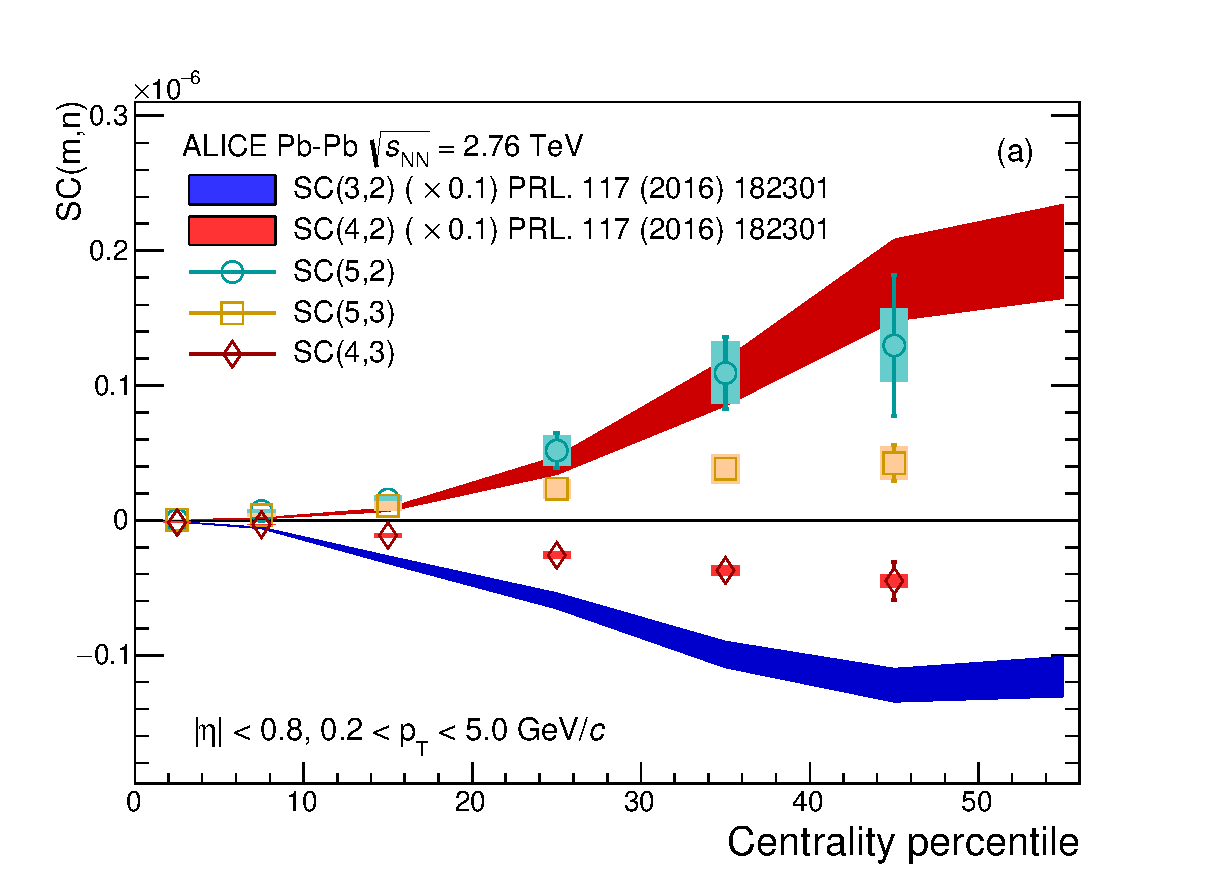
\includegraphics{figs/fig2_QConly_higherSC.eps}}
                       \resizebox{0.48\textwidth}{!}{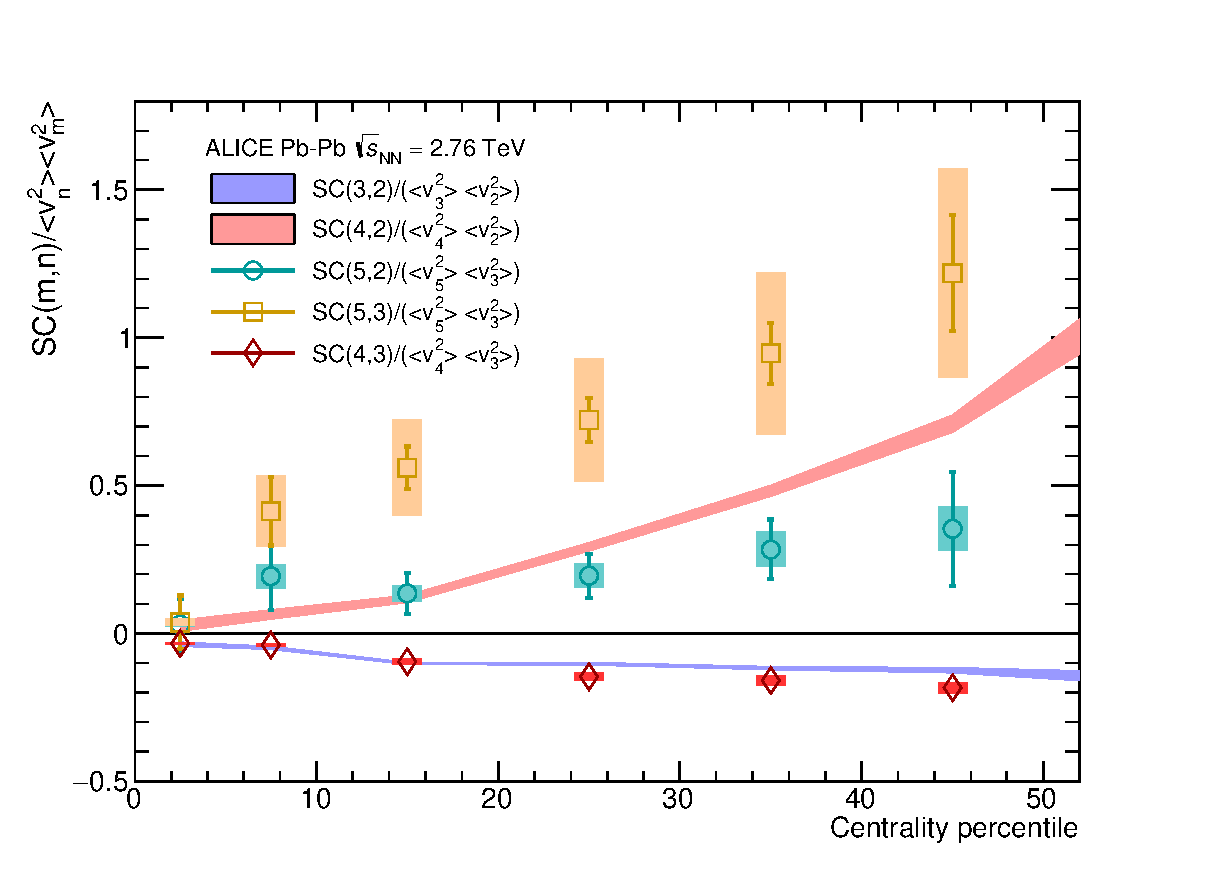
\includegraphics{figs/fig2_QConly_higherNSC.eps}}
        \caption{The result of SC$(m,n)$ (left figure) and NSC$(m,n)$ (right figure) with flow harmonic order up to 5th in $\PbPb$ $\snn=2.76$~TeV. Note that the lower order harmonic correlations (SC(4,2),SC(3,2)) are scaled down by factor of 10 and only statistical errors are shown in the left hand side figure.}
        \label{fig:Figure_1}
              \end{center}
\end{figure}

The centrality dependence of SC(4,2) and SC(3,2) are presented in Fig.~\ref{fig:Figure_1} as shadow bands which are the same as the published results~\cite{ALICE:2016kpq}. Positive values of SC(4,2) are observed for all measured centralities. This suggests a positive correlation between the event-by-event fluctuations of $v_2$ and $v_4$. It also indicates that finding $v_2$ larger than average ($\langle v_2 \rangle$) in an event enhances the probability of finding $v_4$ larger than average ($\langle v_4 \rangle$) in that event. On the other hand, the negative results of SC(3,2) over all measured centralities show the anti-correlation between $v_2$ and $v_3$ flow harmonic magnitudes, which further implies that finding $v_2$ larger than average ($v_2 > \langle v_2 \rangle$) enhancing the probability of finding smaller $v_3$ than average ($v_3 < \langle v_3 \rangle$).

% \begin{figure}[htbp]
%            \begin{center}
%                       \resizebox{0.48\textwidth}{!}{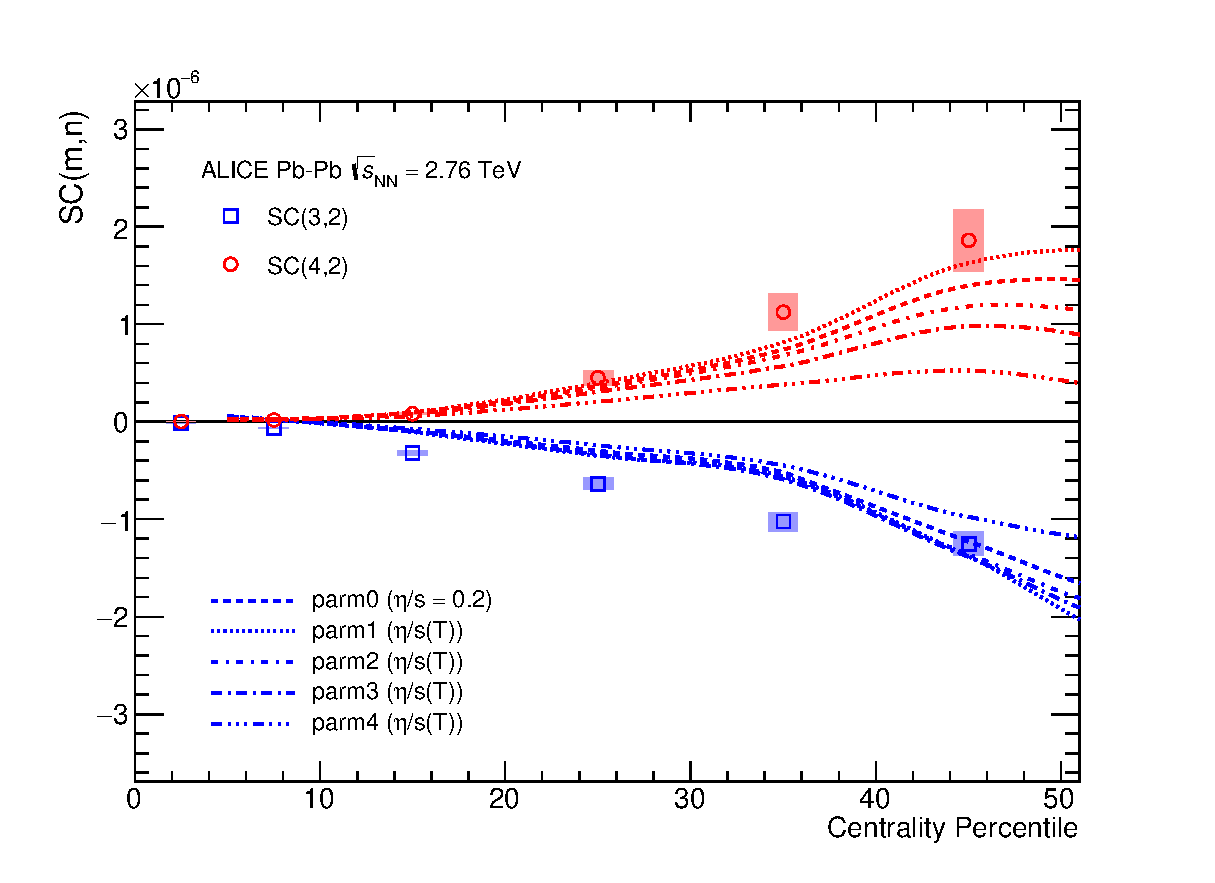
\includegraphics{figs/fig1_QConly.eps}}
%                       \resizebox{0.48\textwidth}{!}{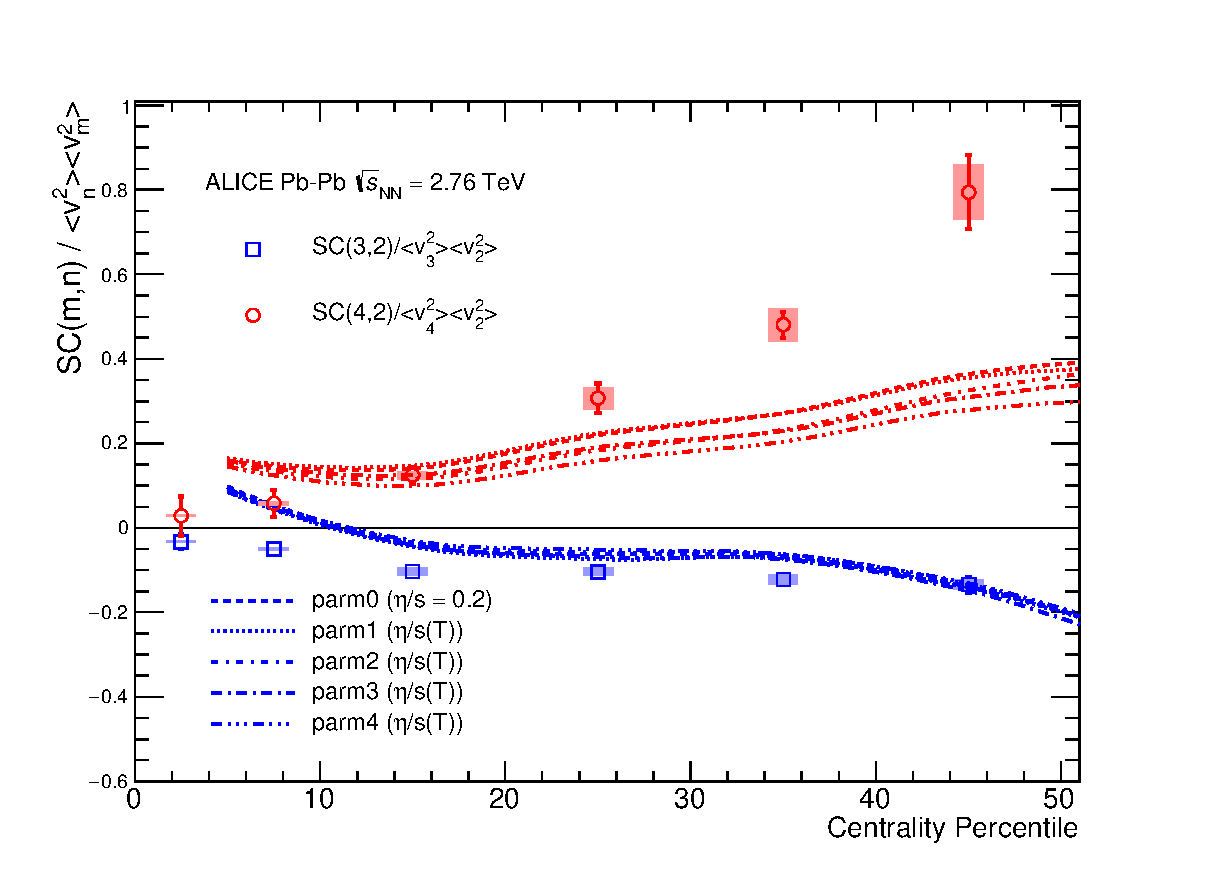
\includegraphics{figs/fig1_QConly_norm.eps}}
%             \caption{The results of SC(3,2)(blue markers) and SC(4,2)(red markers)  with 0.2 $<p_{\rm T}<$ 5.0 GeV/c and $ | \eta | < 0.8$ GeV/$c$ as function of collision centrality (Left). The normalized SC$(m,n)$ (NSC) results which are scaled with $\langle v_m^2 \rangle \langle v_n^2 \rangle $ are shown on the right.}
%              \label{fig:Figure_1}
%              \end{center}
% \end{figure}
 
%\begin{figure}[h]
%	\begin{center}
%       	\resizebox{0.48\columnwidth}{!}{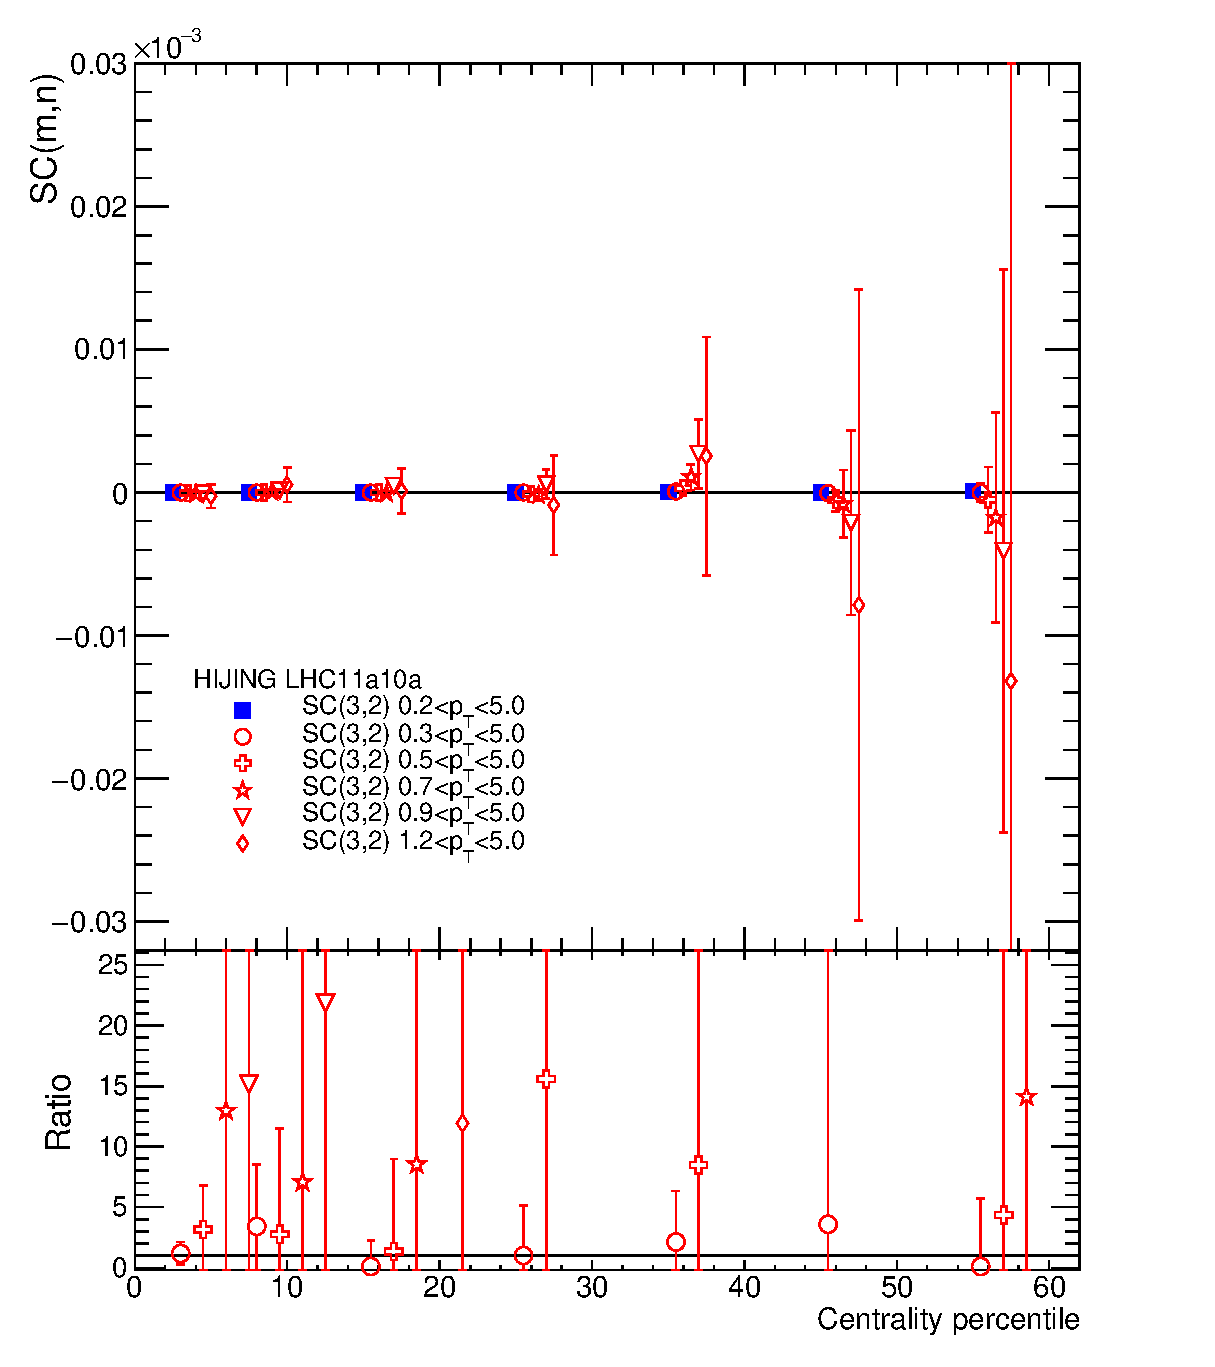
\includegraphics{figs/SC_Comparison_SC32_HIJING_ptdep.eps}}
%        	\resizebox{0.48\columnwidth}{!}{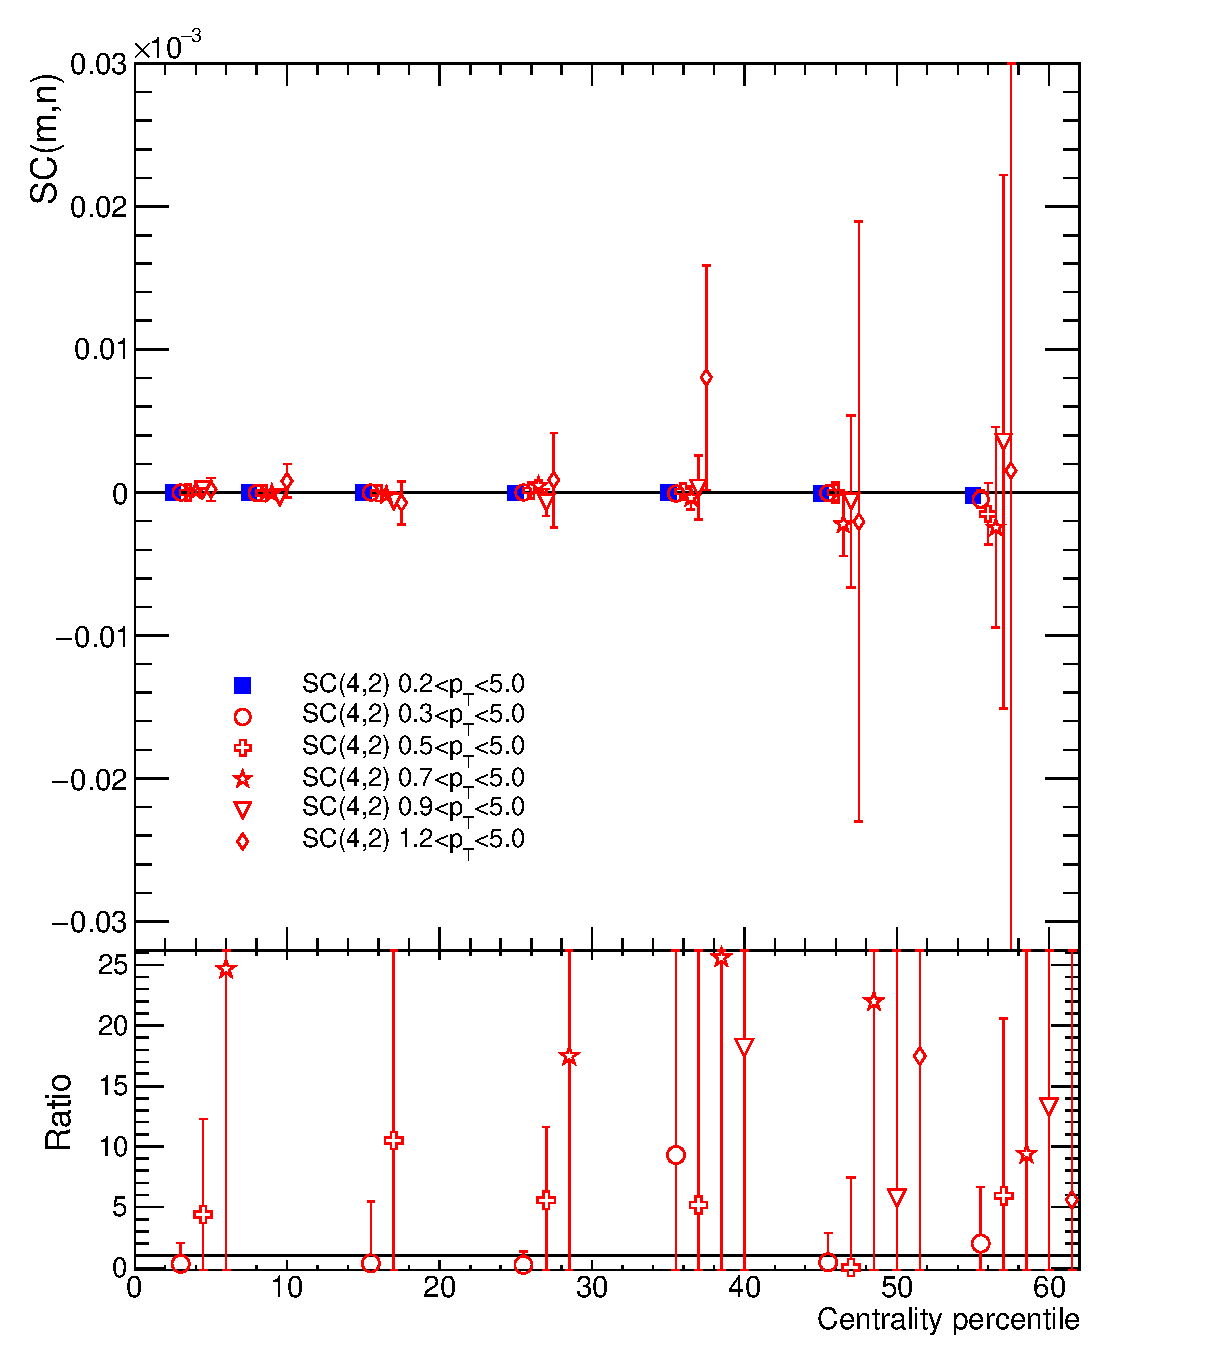
\includegraphics{figs/SC_Comparison_SC42_HIJING_ptdep.eps}}
%        \caption{Result of SC(3,2) and SC(4,2) with HIJING simulations. Defaults($0.2 < p_{\rm T} < 5.0GeV/c$) are drawn as full square with blue color, and different minimum cut conditions are listed in legend. A small shifts along the x axis were applied for better visibility.}
%        \label{fig:results_HIJING}
%        \end{center}   
%\end{figure}

The centrality dependence of the higher order harmonic correlations (SC(4,3), SC(5,2) and SC(5,3)) are presented in Fig.~\ref{fig:Figure_1} and compared to the lower order harmonic correlations (SC(4,2),SC(3,2)). The correlation between $v_3$ and $v_4$ is negative as similarly as $v_3$ and $v_2$ while the others are all positive. 
The higher order flow harmonic correlations (SC(4,3), SC(5,2) and SC(5,3)) are much smaller compared to the lower order harmonics (SC(3,2) and SC(4,2)). Especially SC(5,2) is 10 times smaller than SC(4,2) and SC(4,3) is about 20 times smaller that SC(3,2).

However, unlike SC$(m,n)$, NSC$(m,n)$ results with the higher order flow harmonics show almost same order of the correlation strength as the lower order flow harmonic correlations (NSC(3,2) or NSC(4,2)). NSC(4,3)) is comparable to NSC(3,2) and one finds that a hierarchy NSC(5,3)$>$NSC(4,2)$>$NSC(5,2) holds for most of centrality ranges within the errors.
These results indicate that the lower order harmonic correlations (SC(3,2) and SC(4,2)) are larger than higher order harmonic correlations (SC(4,3), SC(5,2) and SC(5,3)), not only because of the correlation strength itself but also the individual flow strength. 
SC(5,2) is stronger than SC(5,3), but as for NSC, the correlation between $v_5$ and $v_3$ is stronger than the correlation between $v_5$ and $v_2$. 

To obtain the $p_{\rm T}$ dependence of SC$(m,n)$ results, we apply minimum $p_{\rm T}$ cuts, instead of $p_{\rm T}$ bin-by-bin interval in order to avoid large statistical fluctuations in the results. The various minimum $p_{\rm T}$ cuts from 0.2 to 1.5 are applied.
The results of $p_{\rm T}$ dependence with SC(3,2) and SC(4,2) for minimum $p_{\rm T}$ cuts, $0.2<p_{\rm T}<0.7$, are shown on the left top in Fig.~\ref{fig:Figure_2}.
The strength of SC$(m,n)$ correlation becomes larger as the minimum $p_{\rm T}$ increases. This indicates that the relationship between event-by-event fluctuation of two different flow harmonics $v_m$ and $v_n$ is stronger for high $p_{\rm T}$ particles. 
This $p_{\rm T}$ dependence correlations have much stronger centrality dependence, where SC$(m,n)$ gets much larger as the centrality or $p_{\rm T}$ increase. 
NSC(3,2) and NSC(4,2) with different minimum cuts are shown on the right in Fig.~\ref{fig:Figure_2}.
The strong $p_{\rm T}$ dependence observed in SC$(m,n)$ is not clearly seen in NSC$(m,n)$. NSC$(m,n)$ results are aligned all together and consistent in errors for all minimum $p_{\rm T}$ cuts. 
This suggests that the $p_{\rm T}$ dependence of SC$(m,n)$ does not solely result from the correlation between flow harmonics but results from the different values of $p_{\rm T}$  dependent individual $v_n$ values. 
The minimum $p_{\rm T}$ cuts are extended from 0.8  to 1.5 GeV$/c$ and the results are shown on the bottom in Fig.~\ref{fig:Figure_2}.
As for SC$(m,n)$, the similar trends are observed as similarly as $p_{\rm T}<0.8$, however NSC$(m,n)$ tends to decrease as the minimum $p_{\rm T}$ or the centrality increase.
The $p_{\rm T}$ dependence for NSC(3,2) is not clearly seen and it is consistent with no $p_{\rm T}$ dependence within the current statistical and systematic errors except for 40-50\% centrality
and NSC(4,2) shows a moderate decreasing trend for increasing $p_{\rm T}$ (see further discussions in Sec.~\ref{sec:ptdepsc}).
This might be an indication of possible viscous corrections for the equilibrium distribution at hadronic freeze-out~\cite{Luzum:2010ad}.
%However within the current statistical and systematic errors, it is consistent with no $p_{\rm T}$ dependence of NSC$(m,n)$ (see further discussions in Sec.~\ref{sec:ptdepsc}).

\begin{figure}[p]
	\begin{center}
        	\resizebox{0.48\columnwidth}{!}{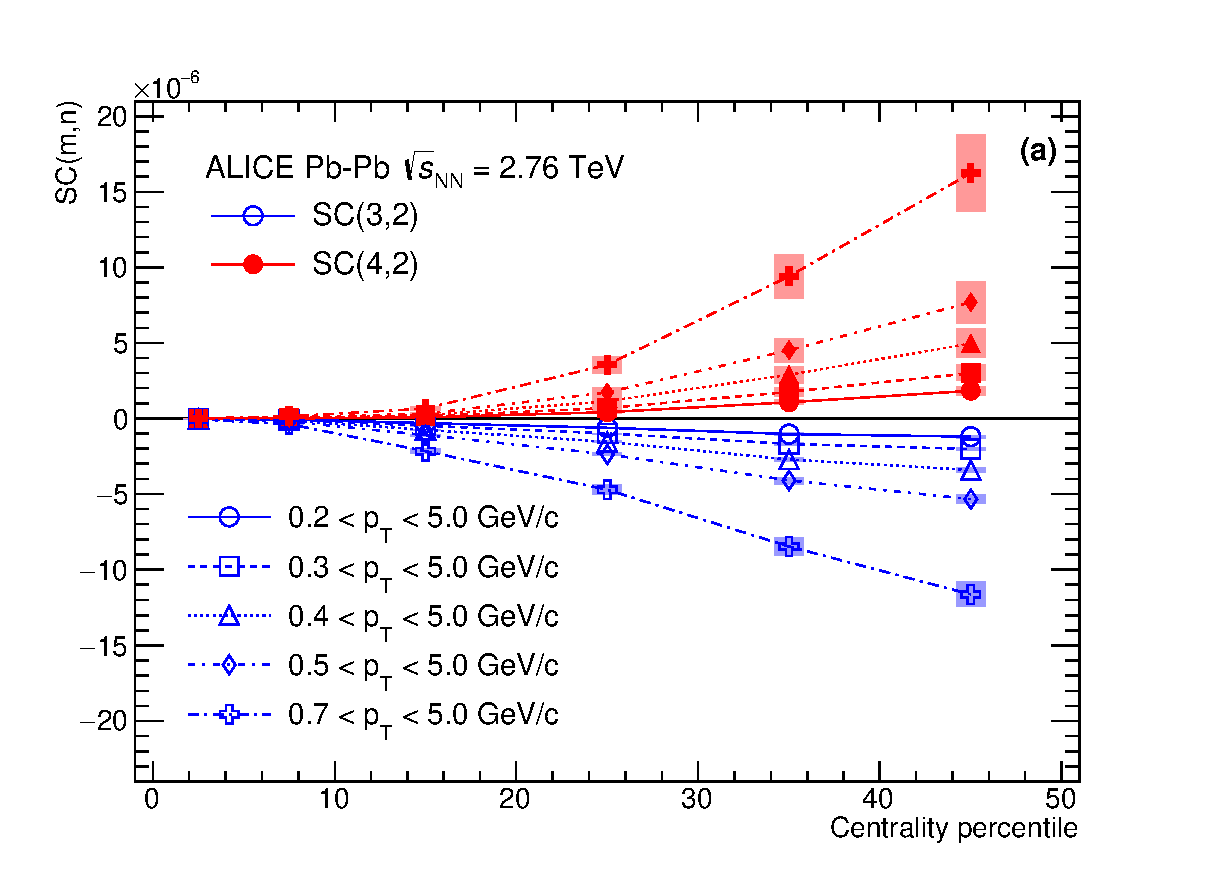
\includegraphics{figs/fig4_QConly_SC_ptdep}}
        	\resizebox{0.48\columnwidth}{!}{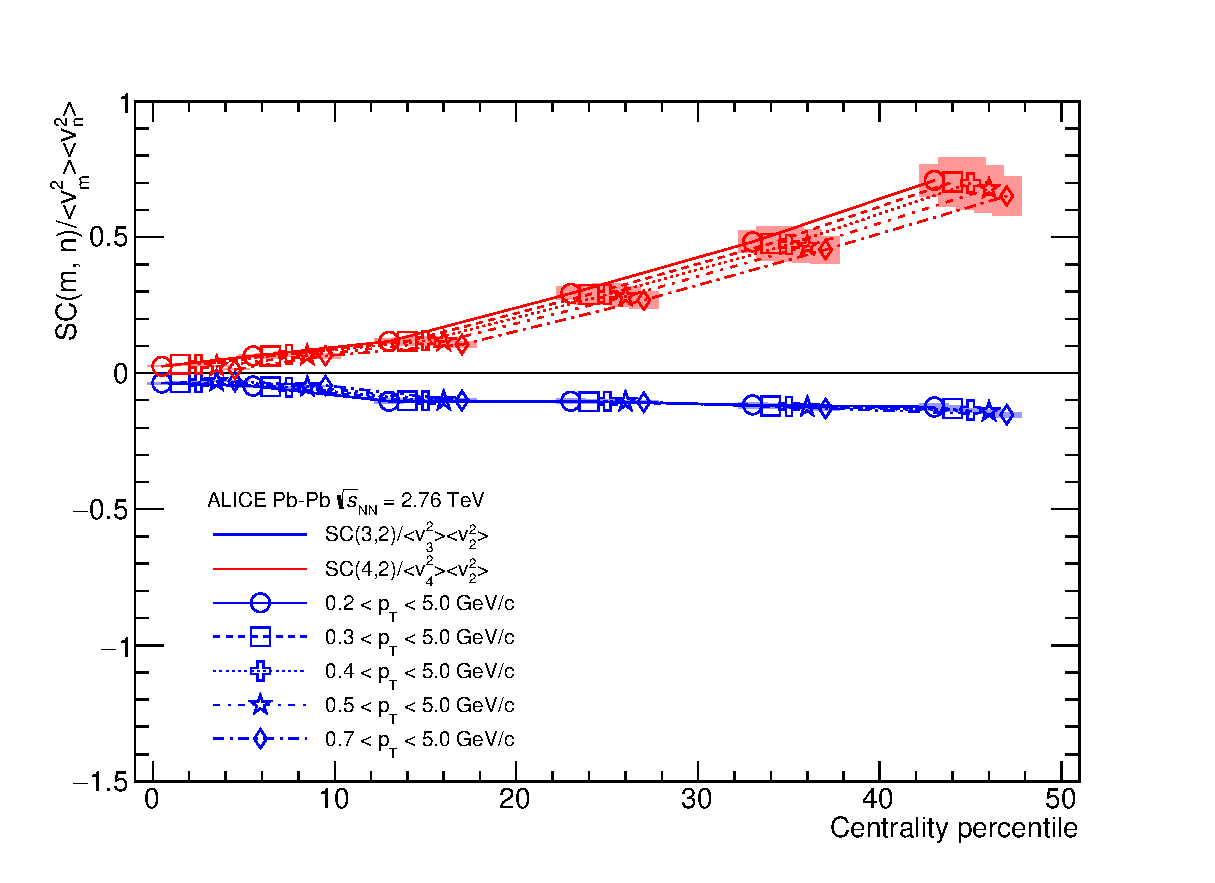
\includegraphics{figs/fig4_QConly_nSC_ptdep}}
	\resizebox{0.48\columnwidth}{!}{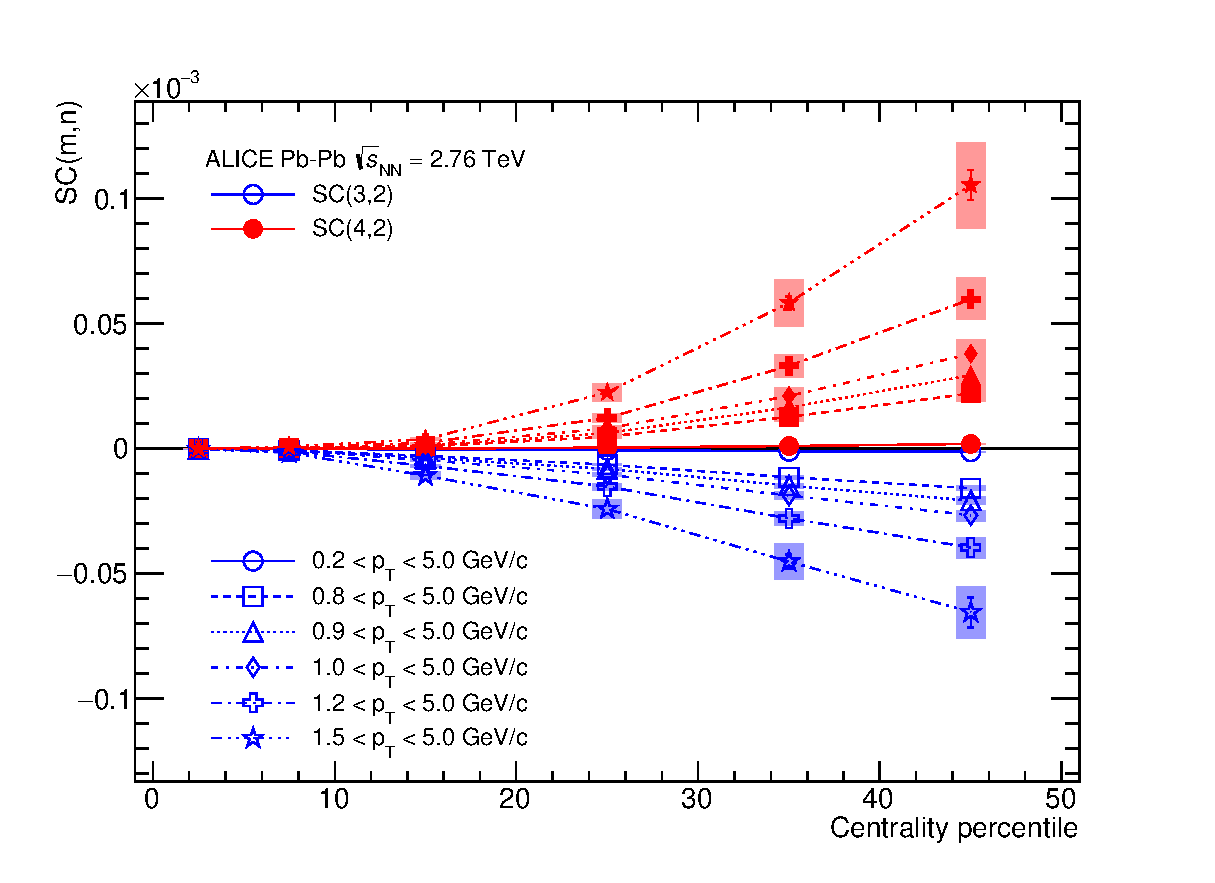
\includegraphics{figs/fig4b_QConly_SC_ptdep}}
        	\resizebox{0.48\columnwidth}{!}{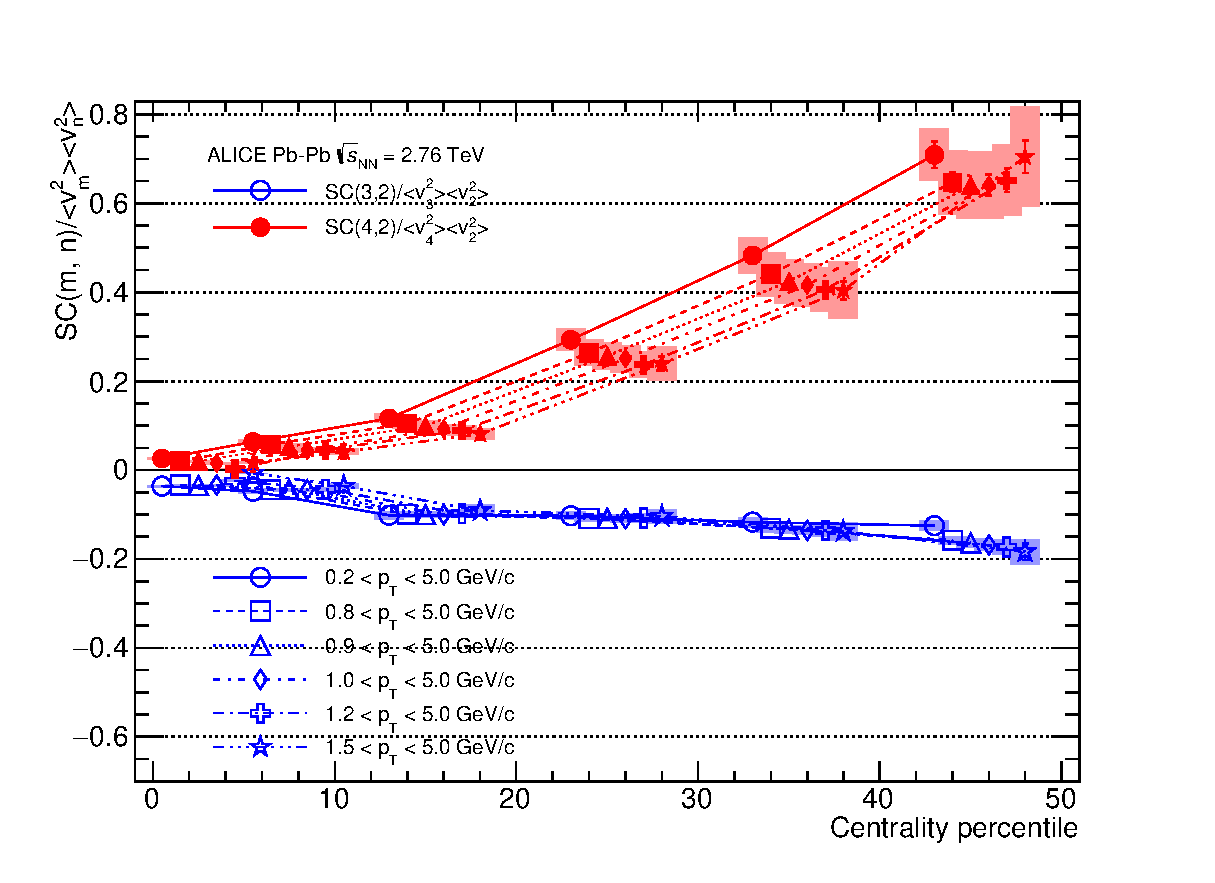
\includegraphics{figs/fig4b_QConly_nSC_ptdep}}
        \caption{SC(3,2) and SC(4,2) with various minimum $p_{\rm T}$ cuts (left) and results of normalized SC(3,2) and SC(4,2) (right). The upper panels show the results for minimum $p_{\rm T}$ range, $0.2<p_{\rm T}<0.7$ GeV$/c$ and the bottom panels are for minimum $p_{\rm T}$ range, $0.8<p_{\rm T}<1.5$ GeV$/c$. Note that NSC data points from each minimum $p_{\rm T}$ in a centrality percentile bin are shifted for visibility.}
        \label{fig:Figure_2}
        \end{center}   
\end{figure}
 
\newpage
\section{Model comparisons}
\label{sec:theory}
\subsection{Low order harmonic correlations}
SC(3,2) and SC(4,2) are compared to several theoretical calculations. First, the fluid hydrodynamic predictions with the different parameterizations for the temperature dependence of the shear viscosity to entropy ratio $\eta/s(T)$ are shown on the left in Fig.~\ref{fig:Figure_3}. The hydrodynamic calculations roughly capture qualitatively the centrality dependence, but not quantitively. Both SC(3,2) with data and hydrodynamics have negative values for all centralities, while SC(4,2) results have positive values over all measured centralities. However, there is no single centrality for which a given $\eta/s(T)$ parameterization describes both SC(3,2) and SC(4,2) simultaneously. On the other hand, the same hydrodynamic calculations capture the centrality dependence of the individual $v_n$ quantitively~\cite{Eskola:2015uda}.

NSC(3,2) and NSC(4,2) are also compared to the same model on the right in Fig.~\ref{fig:Figure_3}. 
While NSC(3,2) does not show sensitivity to  different $\eta/s(T)$ parameterizations,  NSC(4,2) exhibit much better sensitivity
than NSC(3,2) observable and the individual flow harmonics~\cite{Niemi:2015qia}.
These findings indicate that NSC(3,2) observable is sensitive mainly to the initial conditions, while NSC(4,2) observable is sensitive to both the initial conditions and the system properties, which is consistent with the prediction from~\cite{Niemi:2012aj}.
However, the sign of NSC(3,2) is positive in the models in 0-10\% central collisions while it is negative in data.
In the most central collisions the anisotropies originate mainly from fluctuations, i.e.\ the initial ellipsoidal geometry characteristic for mid-central collisions plays little role in this regime. Hence this observation will help to understand the fluctuations in initial conditions better.
NSC(4,2) observable shows better sensitivity for different $\eta/s(T)$ parameterizations, i.e.\ medium property but the model cannot describe the centrality dependence nor the absolute values. These observed distinct discrepancies between data and models might indicate that the current understanding of initial conditions used in the model need to be revisited
to further constrain the $\eta/s(T)$, considering the difficulties on separating the role of the $\eta/s$  from the initial condition to the final state particle anisotropies~\cite{Romatschke:2007mq,Shen:2011zc}.
Hence the use of SC$(m,n)$ and NSC$(m,n)$ can provide new constraints on the detailed modeling of the initial-state condition and the fluctuations of the medium created in heavy-ion collisions and the better constraints on the initial-state conditions will certainly improve the uncertainties of determining $\eta/s(T)$.

\begin{figure}[htbp]
            \begin{center}
                       \resizebox{0.48\textwidth}{!}{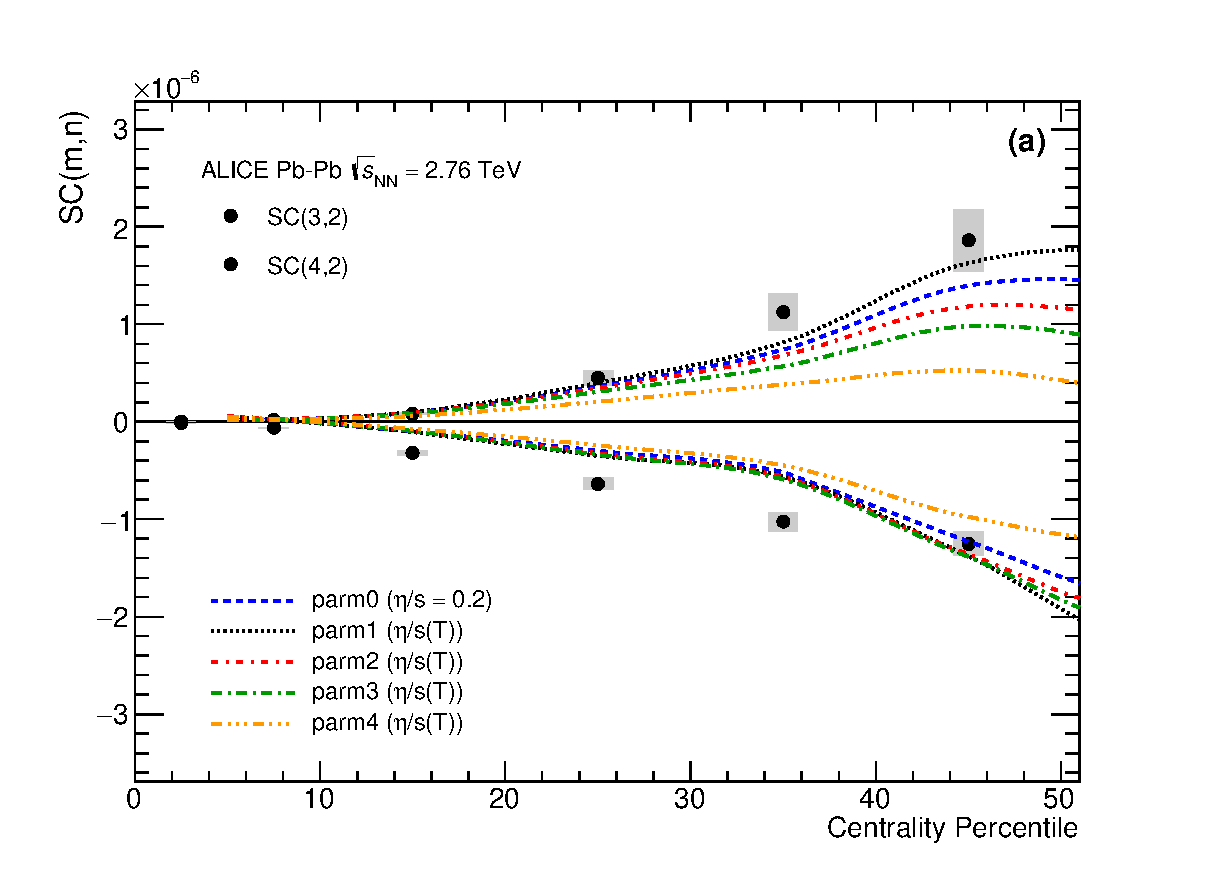
\includegraphics{figs/fig1_QConly_hydro.eps}}
                       \resizebox{0.48\textwidth}{!}{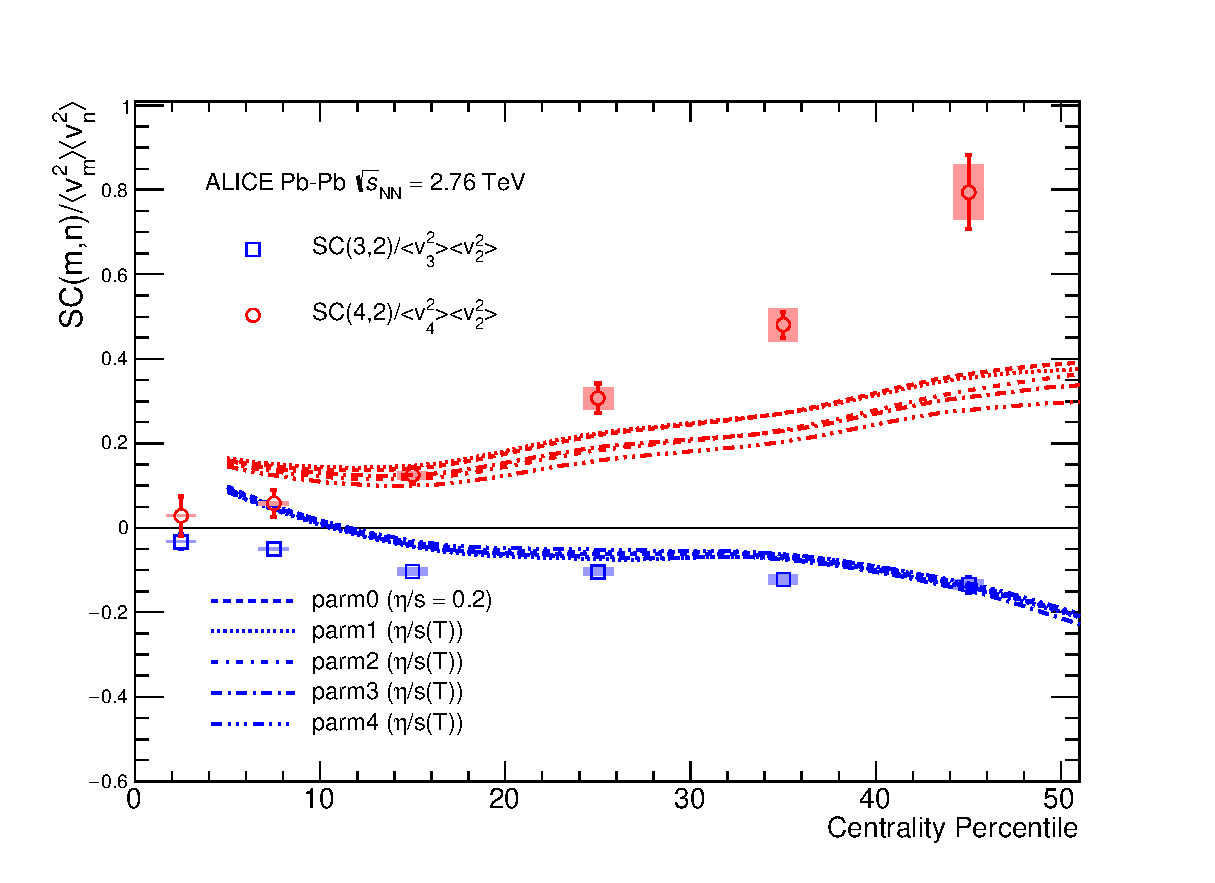
\includegraphics{figs/fig1_QConly_hydro_norm.eps}}
              \end{center}
        \caption{Results from SC(m,n) in $\PbPb$ $\snn=2.76$~TeV are compared to hydrodynamic calculations. The dashed lines are hydrodynamic predictions with various $\eta/s(T)$ parametrizations~\cite{Niemi:2015qia}.}
        \label{fig:Figure_3}
\end{figure}

The results with the comparison to VISH2+1 calculation are shown in Fig.~\ref{fig:Figure_4}.  All the models with the large share viscosity regardless of the initial conditions ($\eta/s=0.2$ for MC-KLN and MC-Glauber initial conditions and $\eta/s=0.16$ for AMPT initial condition) fails to capture the centrality dependence of SC(3,2) and SC(4,2). 
And among the models with small shear viscosities ($\eta/s=0.08$), the one with the AMPT initial condition describes the data better both for SC(3,2) and SC(4,2) but they cannot describe the data quantitively for most of the centrality ranges.
As similarly as the above mentioned hydrodynamic calculations~\cite{Niemi:2015qia}, the sign of the normalised NSC(3,2) in these models is opposite to the data in 0-10\% central collisions. NSC(3,2) does not show sensitivity to initial conditions or $\eta/s$ parametrizations and cannot be described by these models quantitively.
However, for NSC(4,2), it is sensitive both to initial conditions and $\eta/s$ parametrizations.
Even though NSC(4,2) is favoured both by AMPT initial condition with $\eta/s$=0.08 and MC-Glauber initial condition with $\eta/s=0.20$,
SC(4,2) can be only described by smaller $\eta/s$ from AMPT and MC-Glauber initial conditions. Therefore the Glauber initial condition with $\eta/s=0.20$ model can be ruled out and we come to a conclusion based on the tested model parameters that $\eta/s$ should be small and AMPT initial condition is favoured by the data.

\begin{figure}[!p]
	\begin{center}
        	\resizebox{0.48\columnwidth}{!}{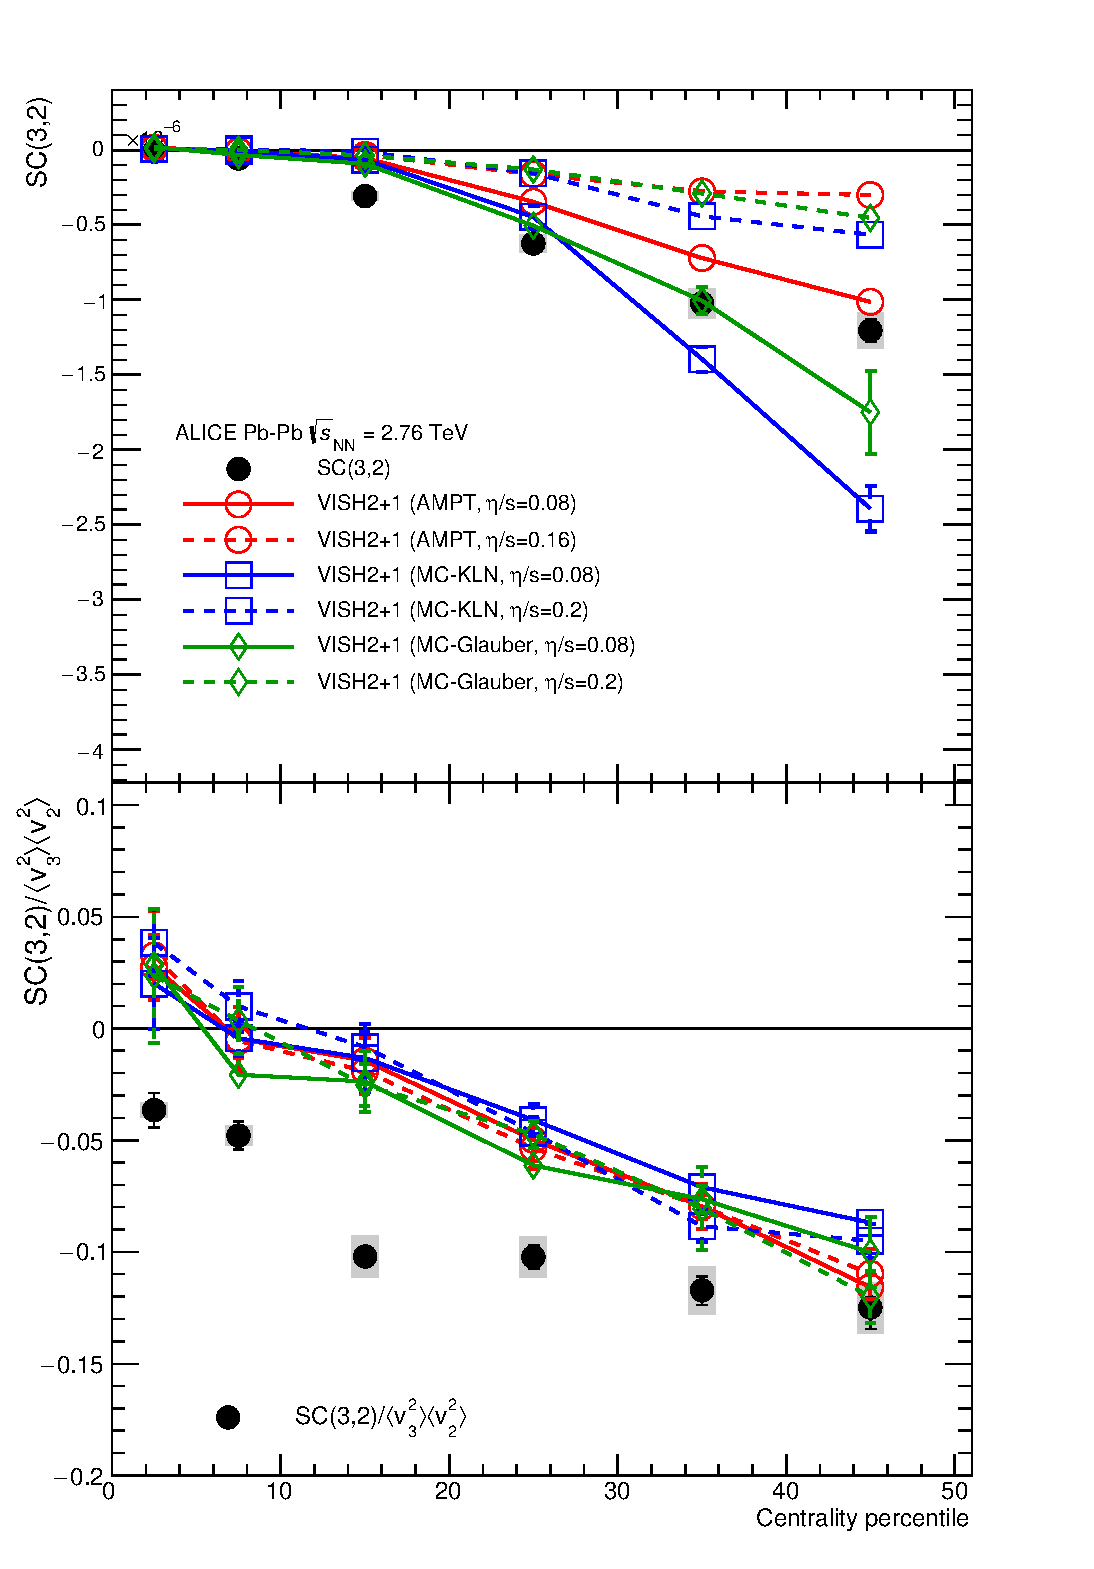
\includegraphics{figs/fig3_QConly_ModelComparison_SC32_vish.eps}}
        	\resizebox{0.48\columnwidth}{!}{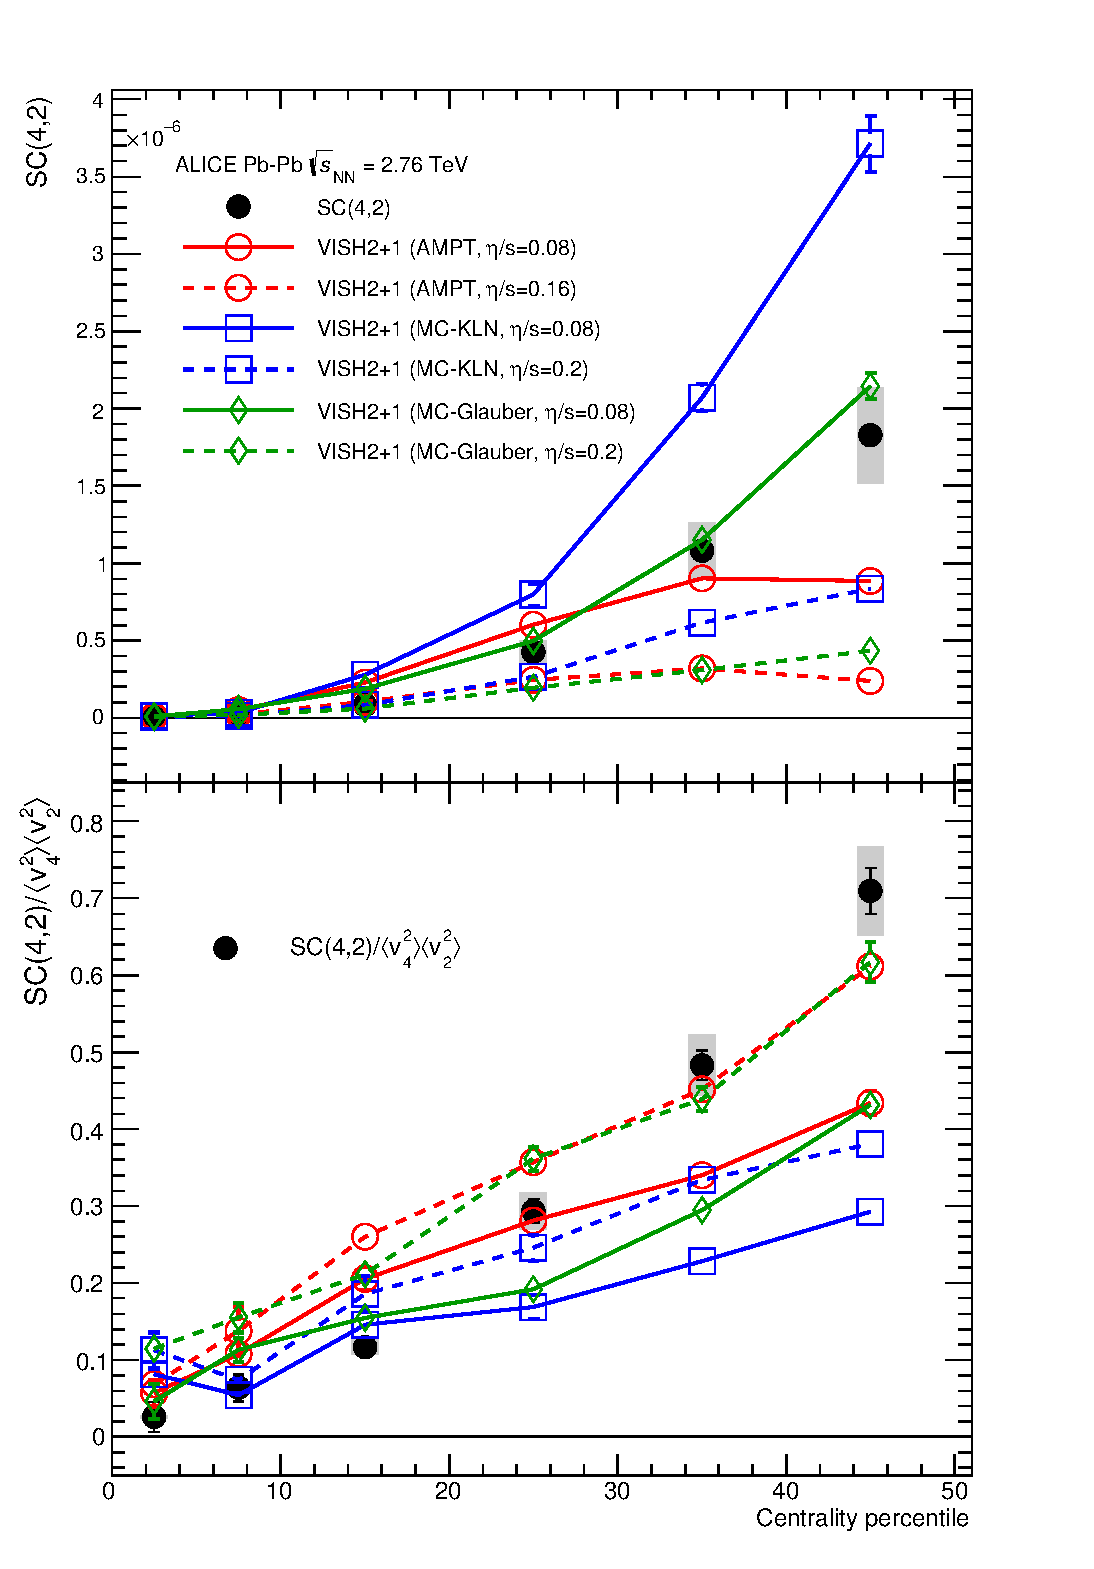
\includegraphics{figs/fig3_QConly_ModelComparison_SC42_vish.eps}}
        \caption{Results of  SC(3,2) and SC(4,2) are compared to various VISH2+1 calculations with different settings. Three initial conditions from AMPT, MC-KLN, and MC-Glauber  are drawn as different colors and markers. The $\eta/s$ parameters are shown as different line styles, the small shear viscosities ($\eta/s=0.08$) are shown as solid lines, and large shear viscosities ($\eta/s=0.2$ for MC-KLN and MC-Glauber, 0.16 for AMPT) are drawn as dashed lines. Upper panels are the result of SC$(m,n)$ and lower panels are the results of NSC$(m,n)$.}
         \label{fig:Figure_4}
        \end{center}   
 \end{figure}
 
Finally, the extracted results  from particle level AMPT simulations in the same way as for the data are compared to the data in Fig.~\ref{fig:Figure_5}.
As for SC(3,2), neither of the settings can describe the data and the setting with the default AMPT model somewhat follows the trend of the data closest. The same setting can describe NSC(3,2) fairly well and also the sign of NSC(3,2) is well reproduced by this setting while all the hydrodynamic calculations in this article failed to describe the sign of the observable in the most central collisions.
Interestingly the string melting AMPT model cannot capture the data well where the strength of the correlation is weaker than the default model.
The third version based on the string melting configuration with the hadronic rescattering phase off is also shown to quantify its influence.
This late hadronic rescattering stage makes both SC(3,2) and NSC(3,2) stronger in the string melting AMPT model but it is not enough to describe the data.
Further we investigated why the default AMPT model can describe NSC(3,2) fairly well but underestimates SC(3,2). By taking the differences in the individual flow harmonics ($v_2$ and $v_3$) between the model and data into account, we were able to recover the difference in SC(3,2) between the data and the model. The discrepancy in SC(3,2) can be explained by the overestimated individual $v_n$ values reported in \cite{Adam:2016nfo} in all the centrality ranges. 

In the case of SC(4,2), the string melting AMPT model can fairly well describe the data while the default model underestimates it.
NSC(4,2) is slightly overestimated by the same setting which can describe SC(4,2) but the default AMPT model can describe the data better.
The influence of the hadronic rescattering phase for NSC(4,2) is opposite to other observables (SC(3,2), NSC(3,2) and SC(4,2)), where the hadronic rescattering make NSC(4,2) slightly smaller.
It should be noted that the better agreement for SC$(m,n)$ should not be overemphasized since there are discrepancies in the individual $v_n$ between AMPT and data as it was demonstrated for SC(3,2).
Hence the simultaneous description of SC$(m,n)$ and NSC$(m,n)$ should give better constraints to the parameters in AMPT.


\begin{figure}[p]
	\begin{center}
        	\resizebox{0.48\columnwidth}{!}{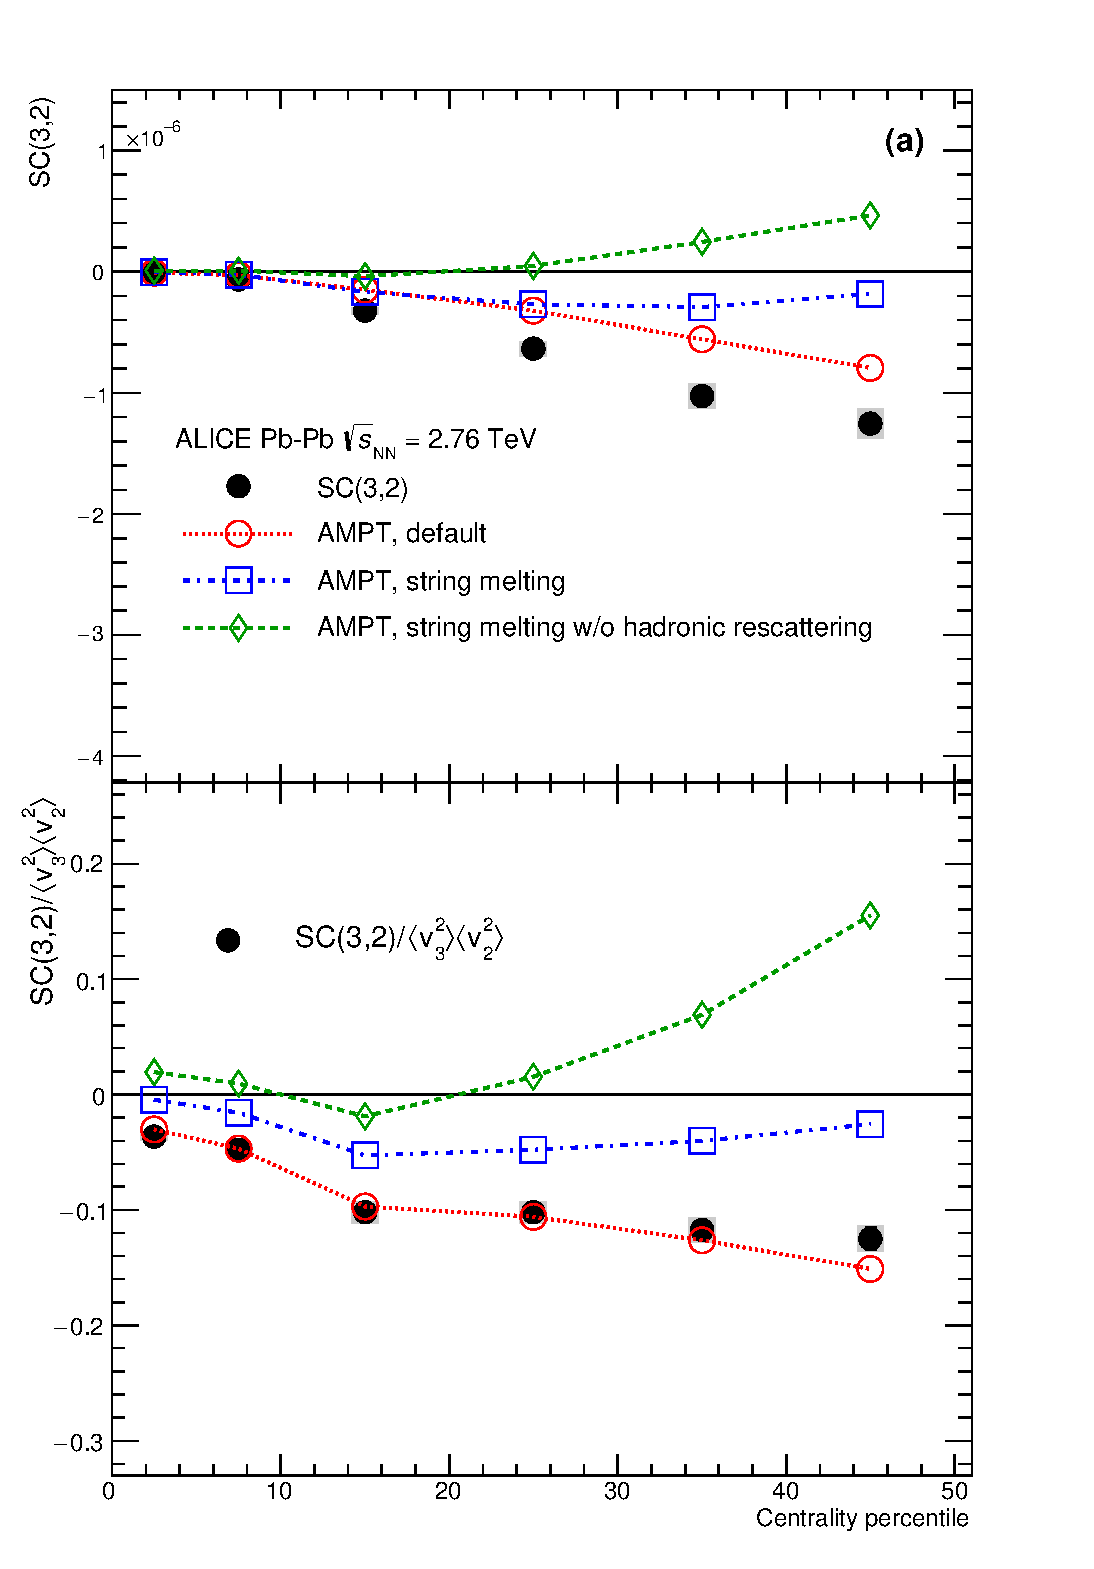
\includegraphics{figs/fig3_QConly_ModelComparison_SC32_ampt.eps}}
        	\resizebox{0.48\columnwidth}{!}{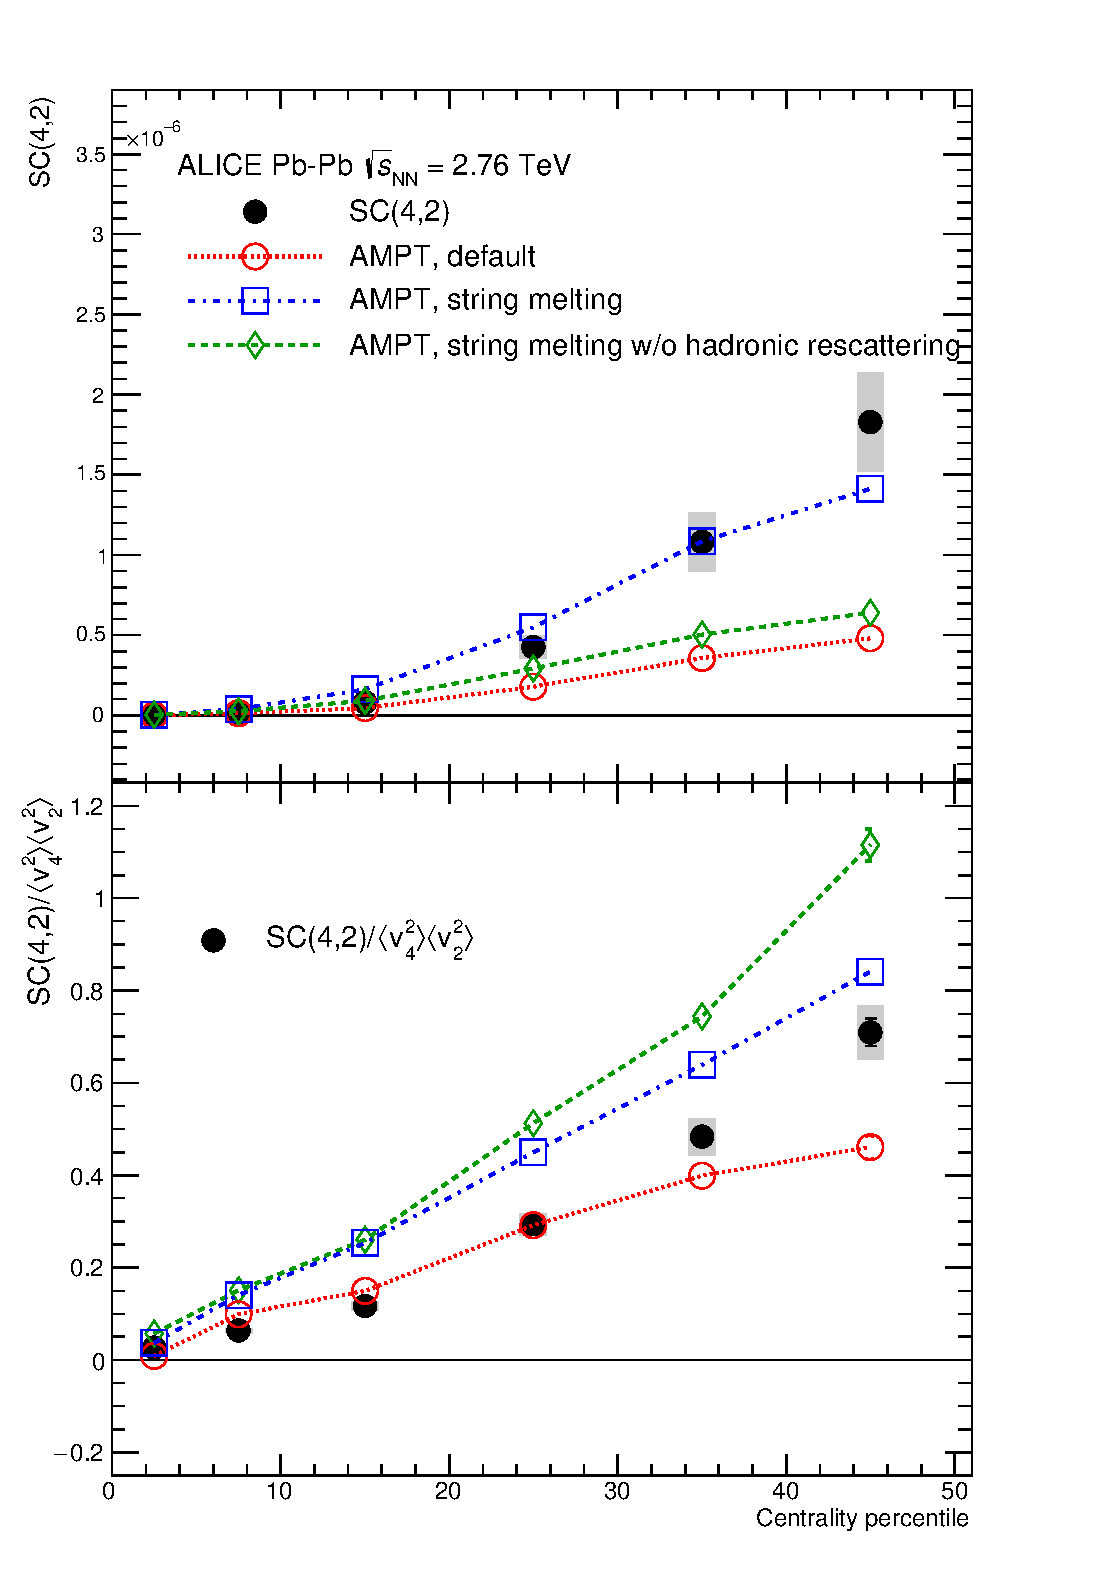
\includegraphics{figs/fig3_QConly_ModelComparison_SC42_ampt.eps}}
        \caption{Results of  SC(3,2) and SC(4,2) are compared to various AMPT simulations. Upper panels are the results of SC$(m,n)$ and the lower panels are the results of NSC$(m,n)$. The details of the AMPT configurations can be found in Sec.~\ref{sec:models}.}
        \label{fig:Figure_5}
        \end{center}   
 \end{figure}
 
 \newpage
\subsection{Higher order harmonic correlations}
The higher order harmonic correlations (SC(4,3), SC(5,2) and SC(5,3)) are compared to VISH2+1 calculation, shown in Fig.~\ref{fig:Figure_6}. 
All the models with the large share viscosity regardless of the initial conditions ($\eta/s=0.2$ for MC-KLN and MC-Glauber initial conditions, and $\eta/s=0.16$ for AMPT) failed to capture the centrality dependence of SC(5,2), SC(5,2) and SC(5,3), more clearly than lower order harmonic correlations (SC(3,2), SC(4,2)).
And among the models with small shear viscosity ($\eta/s=0.08$), the one from the AMPT initial condition describes the data much better than the other initial conditions. 
A quite clear separation between different initial conditions is observed for these higher order harmonics correlations compared to the lower order harmonic correlations.
NSC(5,2) and SC(5,3) are quite sensitive to both the initial conditions and the $\eta/s$ parametrizations.
As similarly as the above mentioned hydrodynamic calculations~\cite{Niemi:2015qia}, the sign of the normalised NSC(4,3) in these models is opposite to the data in 0-10\% central collisions. NSC(4,3) shows sensitivity to both initial conditions and $\eta/s$ parametrizations while NSC(3,2) didn't show sensitivity to initial conditions or $\eta/s$ parametrizations.
SC(4,3) data is clearly favoured by smaller $\eta/s$ but NSC(4,3) cannot be described by these models quantitively.
     
\begin{figure}[p]
	\begin{center}
        	\resizebox{0.32\columnwidth}{!}{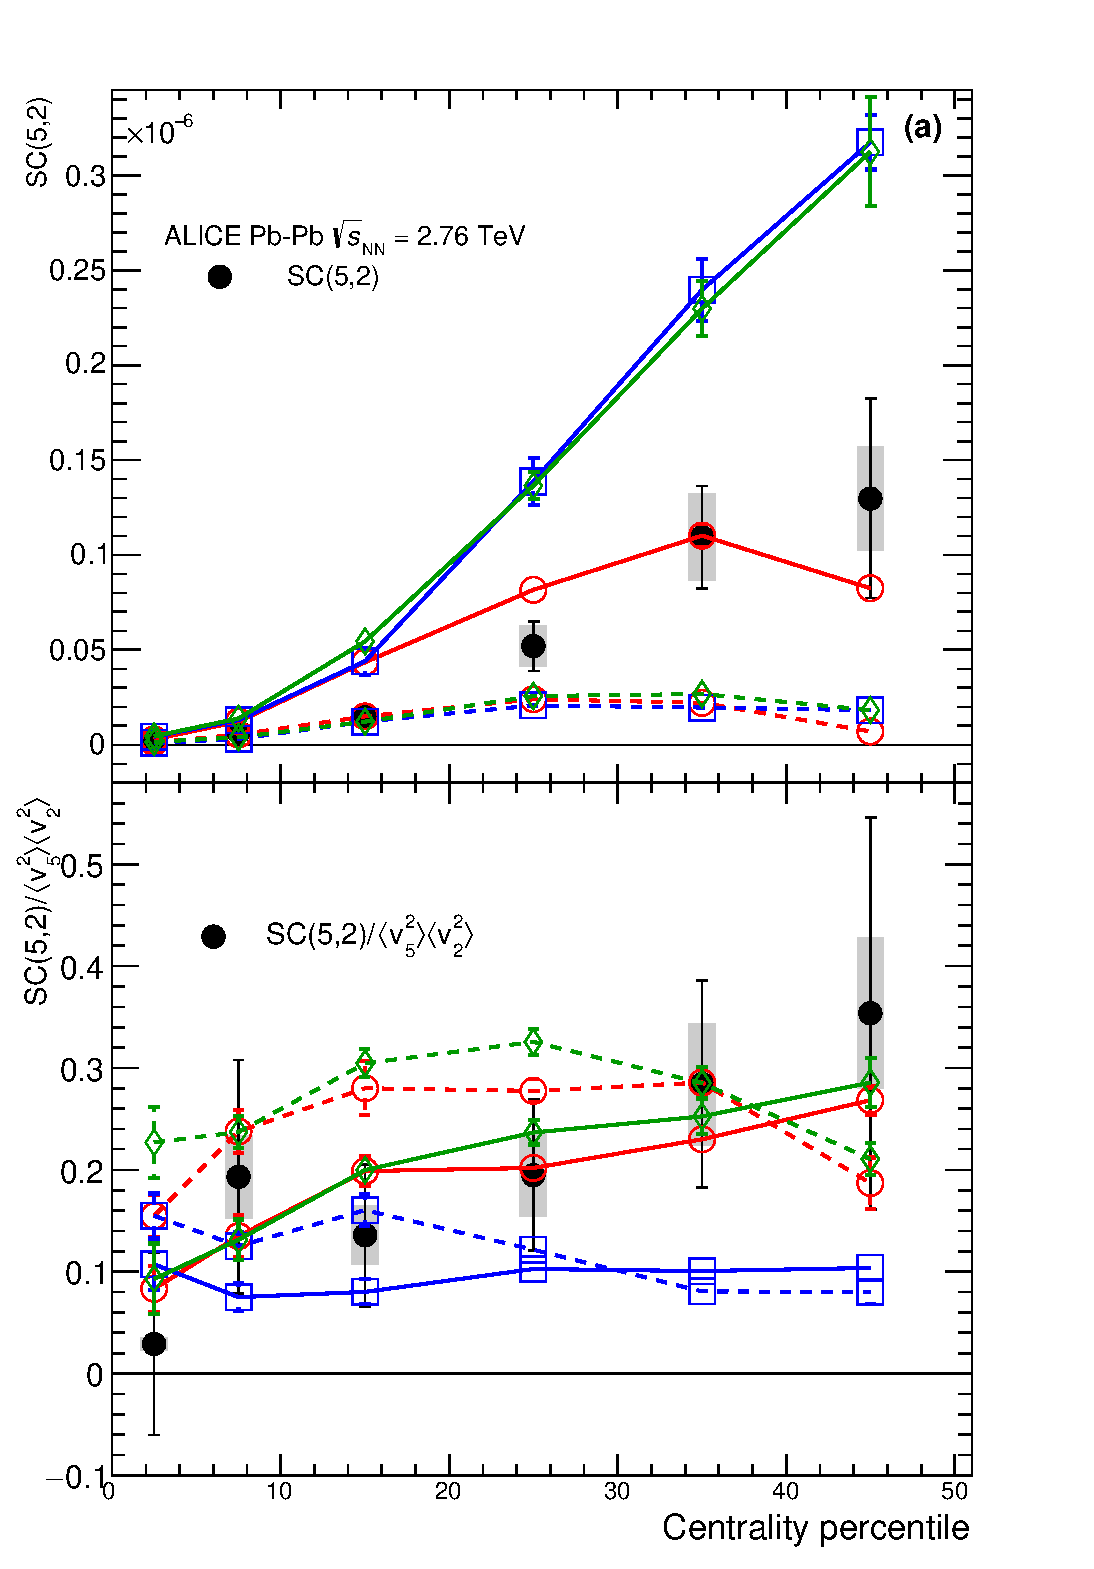
\includegraphics{figs/fig3_QConly_ModelComparison_SC52_vish.eps}}
        	\resizebox{0.32\columnwidth}{!}{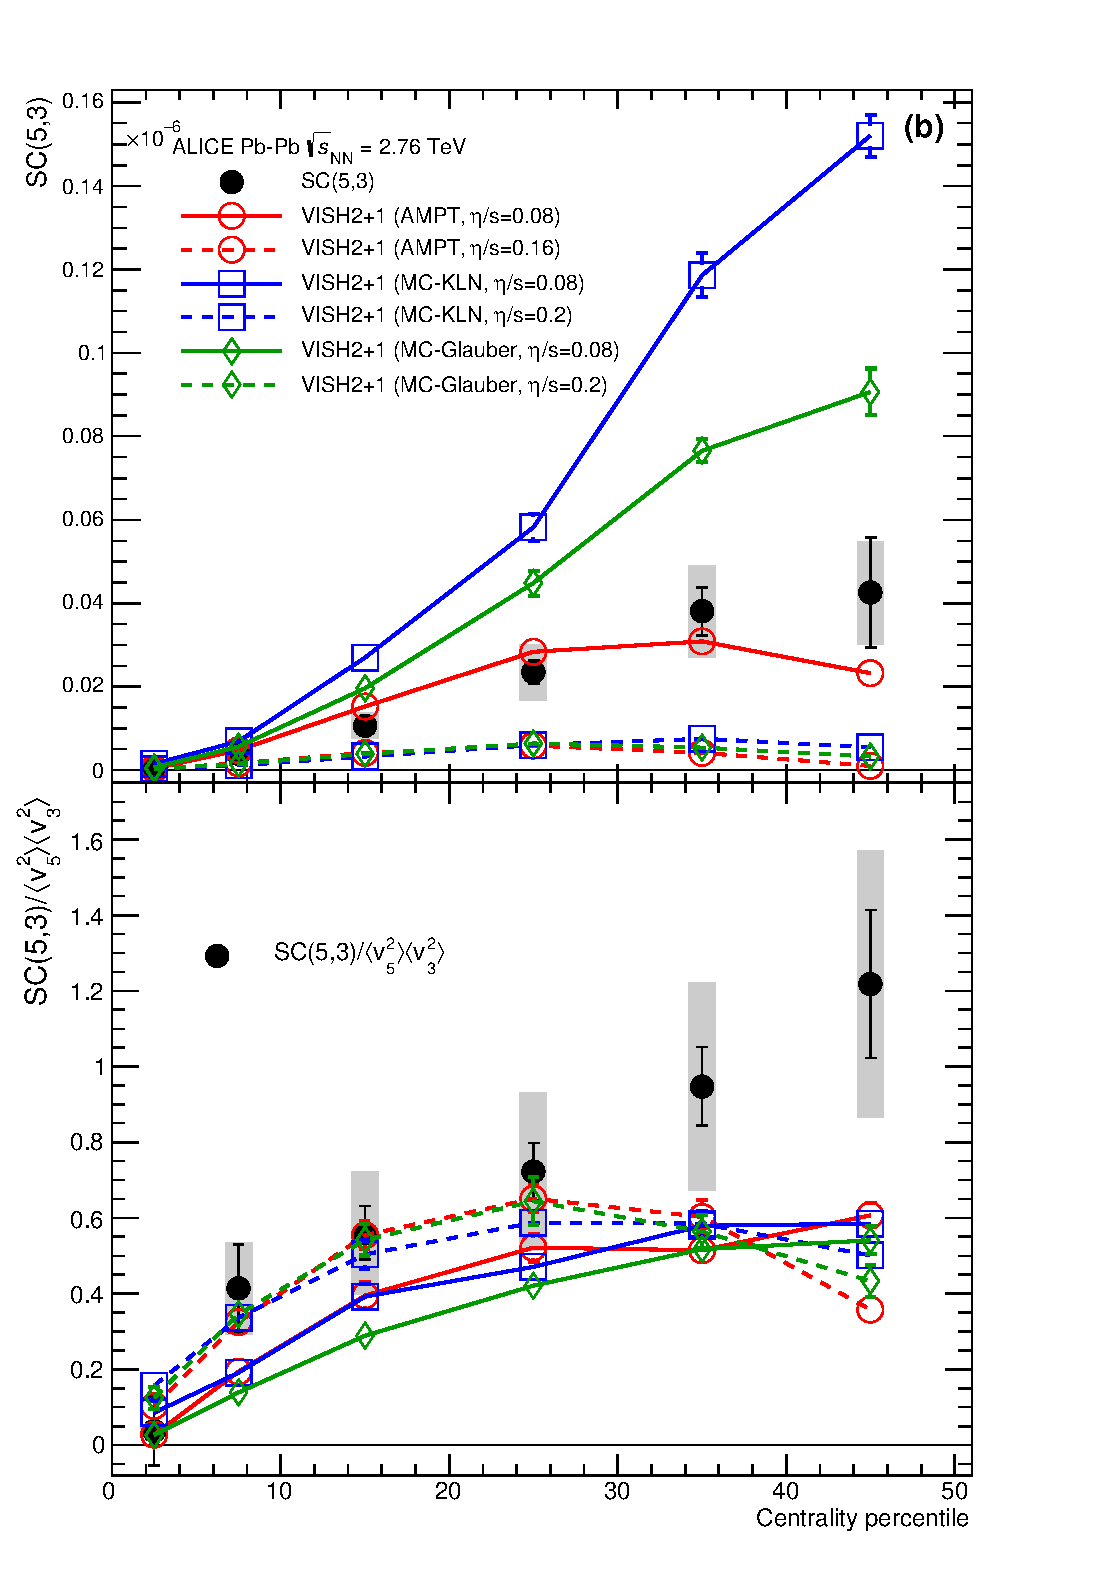
\includegraphics{figs/fig3_QConly_ModelComparison_SC53_vish.eps}}
        	\resizebox{0.32\columnwidth}{!}{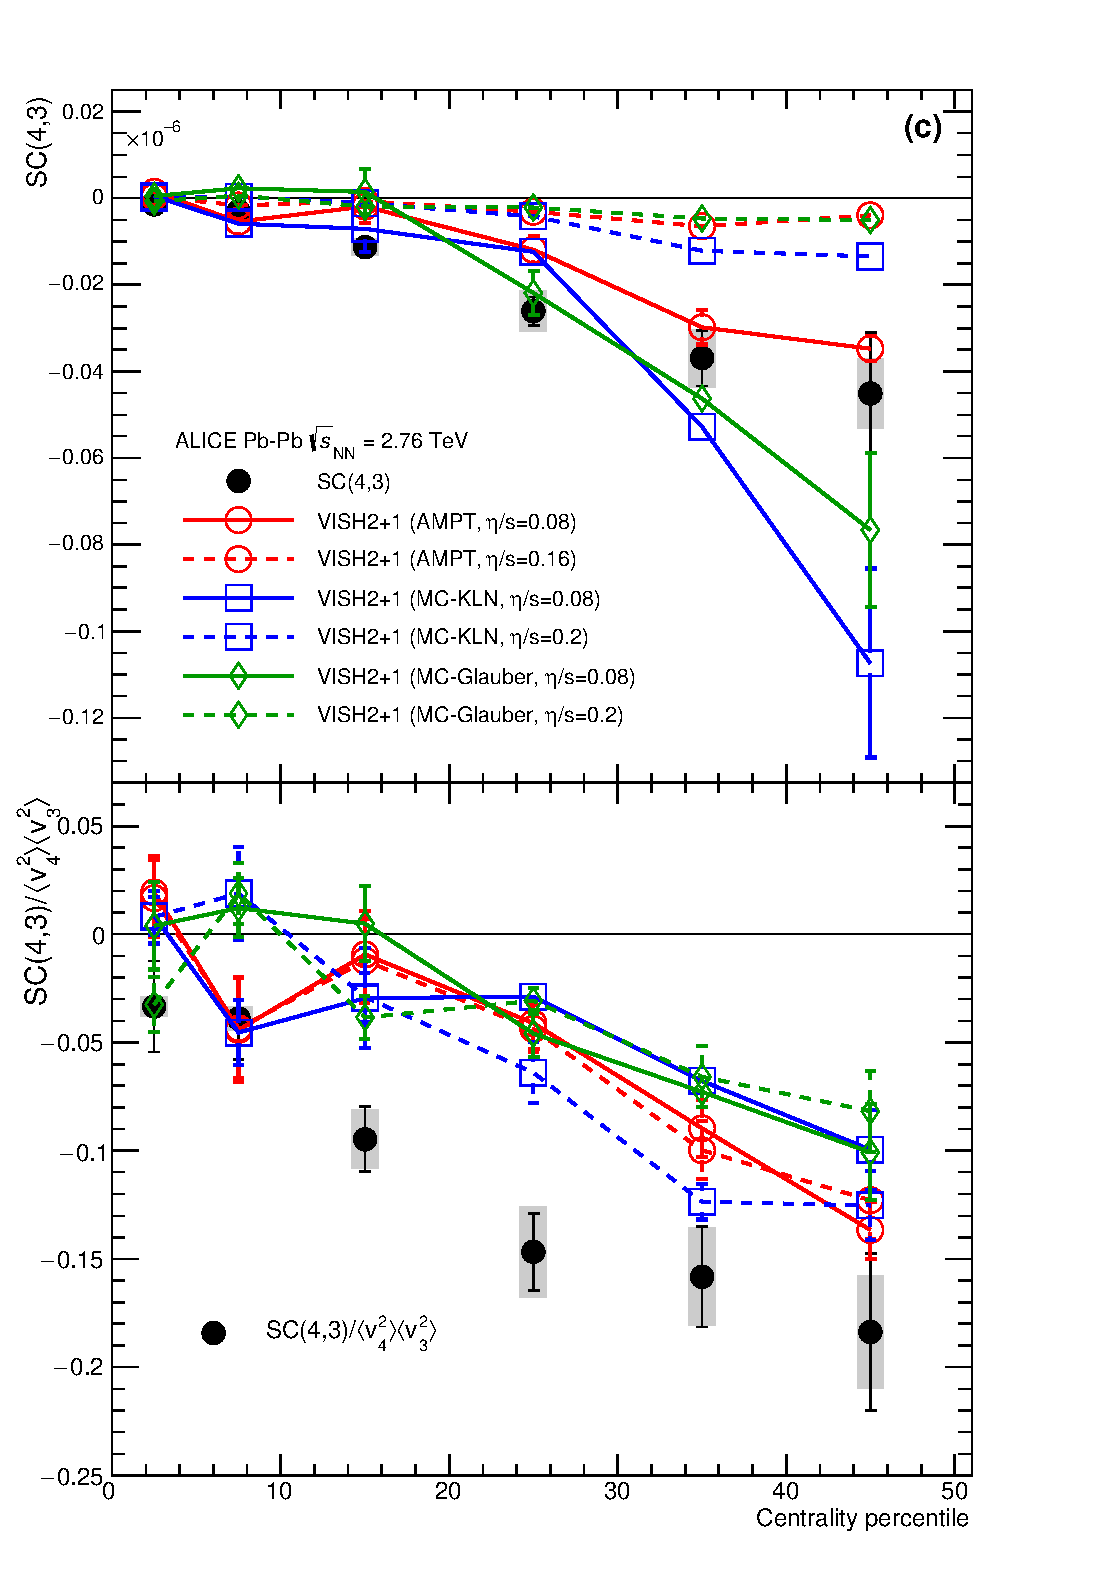
\includegraphics{figs/fig3_QConly_ModelComparison_SC43_vish.eps}}
        \caption{Results of  SC(5,2), SC(5,3) and SC(4,3) are compared to various VISH2+1 calculations. Three initial conditions from AMPT, MC-KLN and MC-Glauber are drawn as different colors and markers. The $\eta/s$ parameters are shown as different line styles, the small shear viscosity ($\eta/s=0.08$) are shown as solid lines, and large shear viscosities ($\eta/s=0.2$ for MC-KLN and MC-Glauber, 0.16 for AMPT) are drawn as dashed lines. Upper panels are the results of SC$(m,n)$ and lower panels are the results of NSC$(m,n)$.}
        \label{fig:Figure_6}
        \end{center}   
 \end{figure}
 
The extracted results  from particle level AMPT simulations in the same way as for the data are compared to the data in Fig.~\ref{fig:Figure_7}.
The string melting AMPT model describes SC(5,2) and SC(5,3) well. The same setting describes only NSC(5,3) but it overestimates NSC(5,2). 
However the default AMPT model can describe NSC(5,3) and NSC(5,2) fairly well as similarly as NSC(3,2) and NSC(4,2).
% intersting AMPT String Melting OFF, Rescatering ON < AMPT String Melting ON, Rescatering OFF
in the case of SC(4,3), neither of the settings can describe the data but the default AMPT model follows the data closest. 
The string melting AMPT model fails to describe SC(4,3) and NSC(4,3).
In summary, the default AMPT model describes the normalized SC (NSC$(m,n)$) from lower to higher order harmonic correlation while the string melting AMPT model overestimates NSC(5,2) and 
underestimates (or very weak correlations) NSC(4,3). 

%It should be noted that the better agreement for SC$(m,n)$ should not be overemphasized since there are discrepancies in the individual $v_n$ between AMPT and data as it was demonstrated for SC(3,2).
%Hence the simultaneous description of SC$(m,n)$ and NSC$(m,n)$ should give better constrains to the parameters in AMPT.
%Can we conclude that the hadronic rescattering only can reproduce the correlation strength well ?
%Considering the underestimated $NSC(4,3)$ in VISH2+1 calculation can be compensated by hadronic rescattering a.l.a ...... ?

\begin{figure}[p]
	\begin{center}
        	\resizebox{0.32\columnwidth}{!}{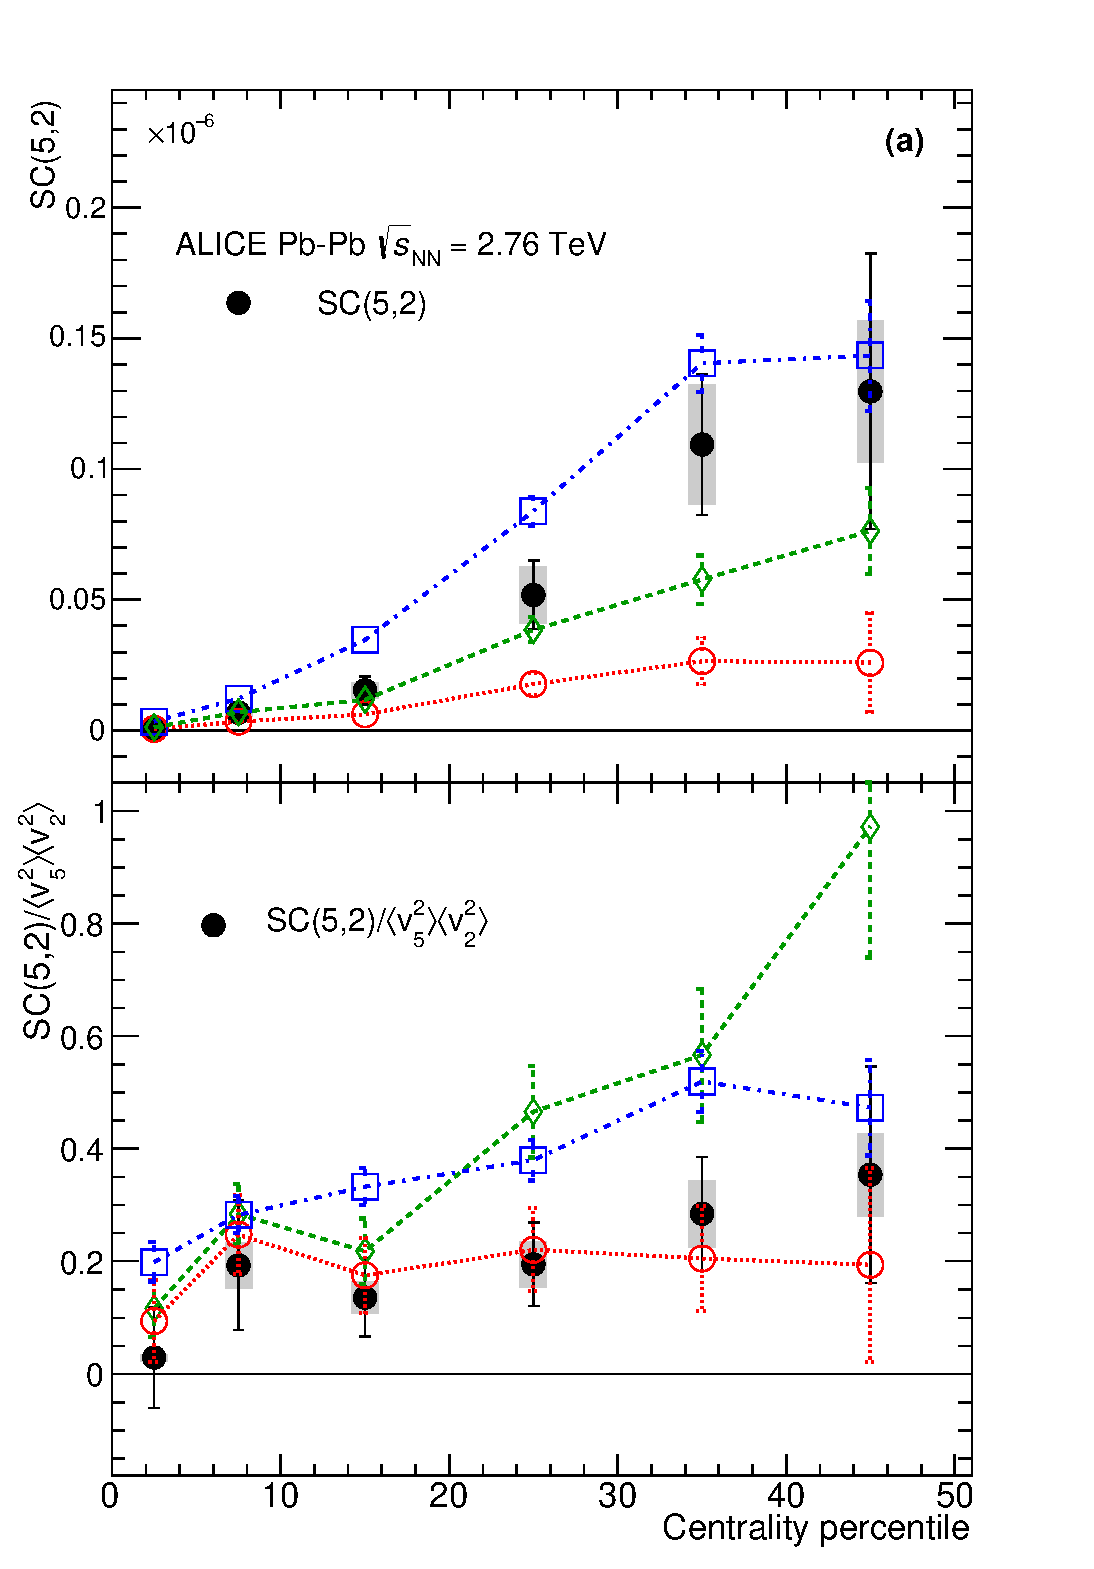
\includegraphics{figs/fig3_QConly_ModelComparison_SC52_ampt.eps}}
        	\resizebox{0.32\columnwidth}{!}{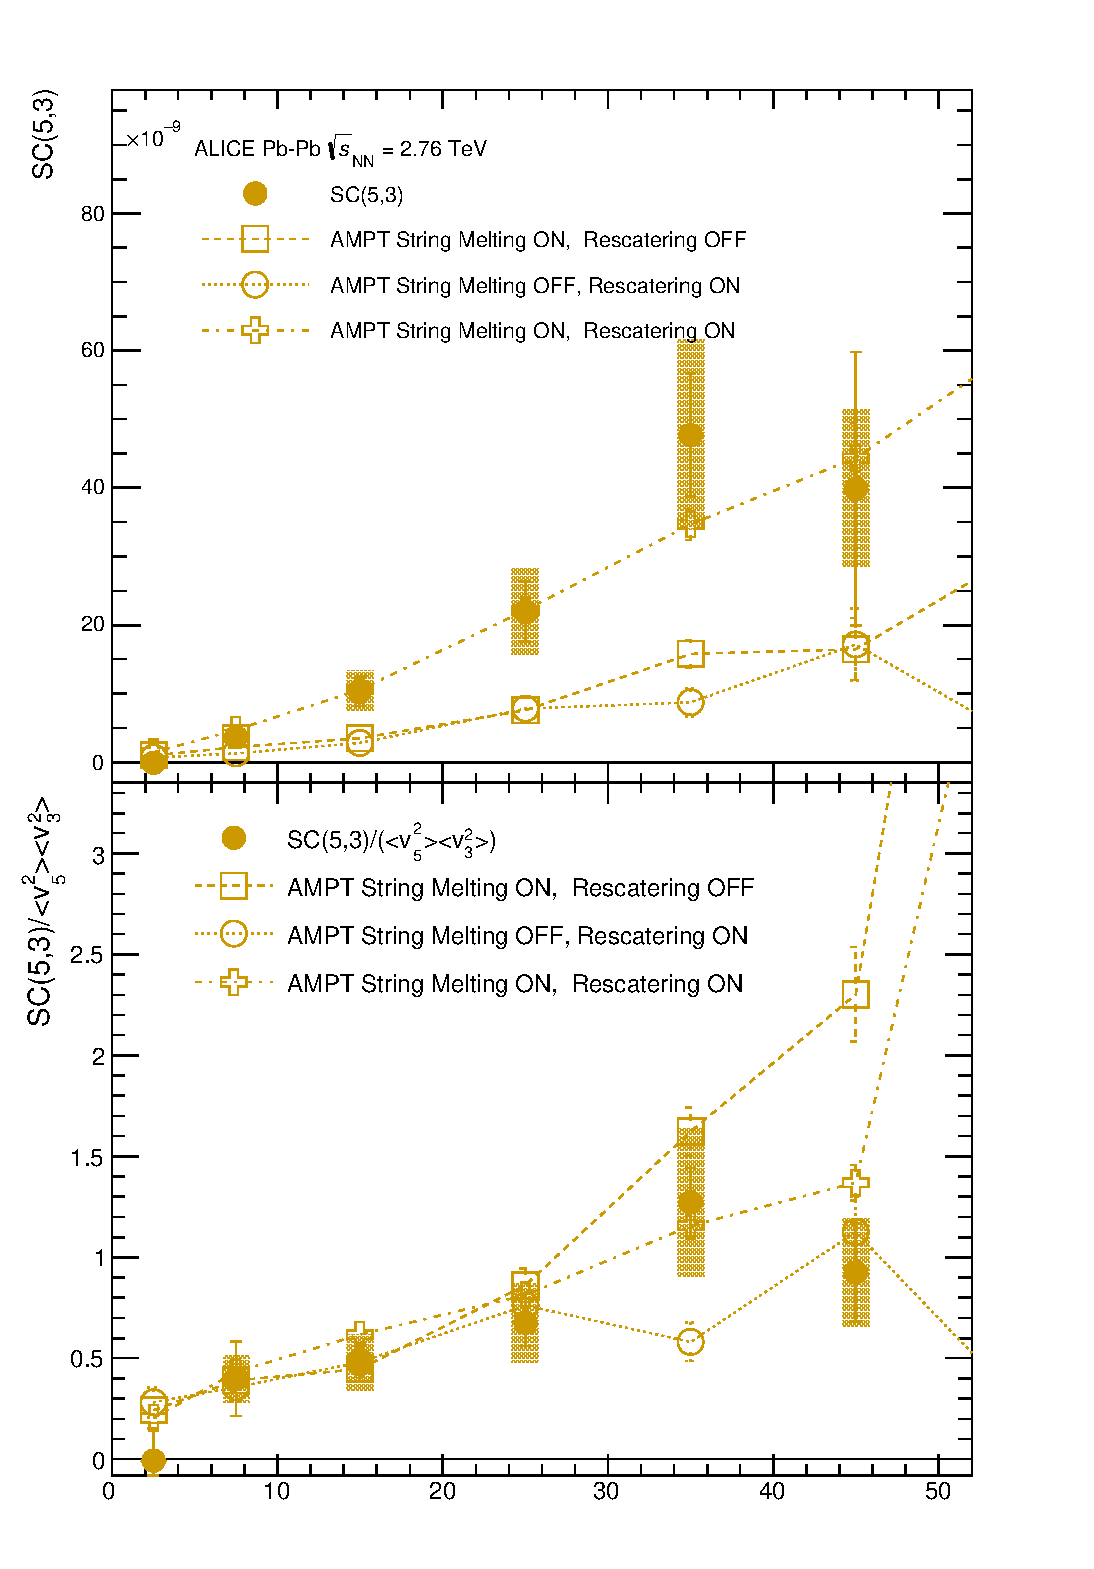
\includegraphics{figs/fig3_QConly_ModelComparison_SC53_ampt.eps}}
        	\resizebox{0.32\columnwidth}{!}{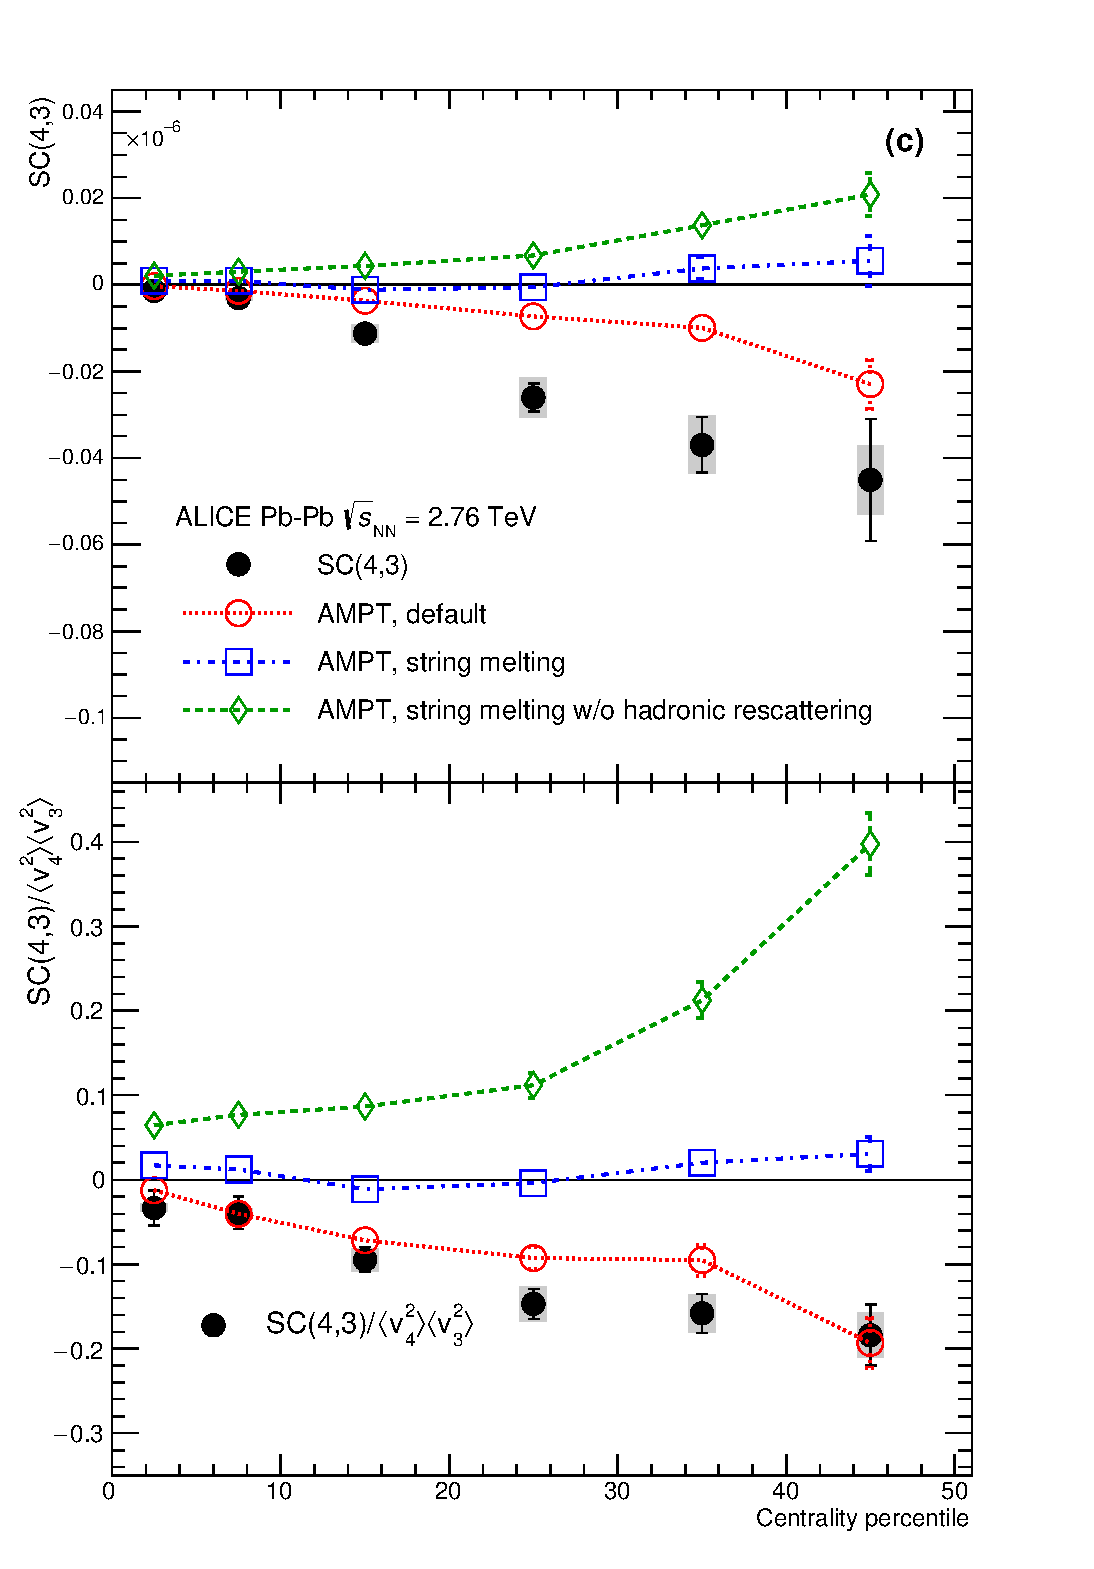
\includegraphics{figs/fig3_QConly_ModelComparison_SC43_ampt.eps}}
        \caption{Results of  SC(5,2), SC(5,3) and SC(4,3) are compared to various AMPT simulations. Upper panels are the results of SC$(m,n)$ and the lower panels are the results of NSC$(m,n)$. The details of the AMPT configurations can be found in Sec.~\ref{sec:models}.}
        \label{fig:Figure_7}
        \end{center}   
 \end{figure}
 
 \newpage
\subsection{Transverse momentum dependence of Low order harmonic correlations}
\label{sec:ptdepsc}
NSC(3,2) and NSC(4,2) as a function of different minimum $p_{\rm T}$ cut are compared to the {AMPT} simulations in Fig.~\ref{fig:Figure_8}.
As discussed in Sec.~\ref{sec:results}, the $p_{\rm T}$ dependence for NSC(3,2) and NSC(4,2) in mid central collisions is seen also in AMPT simulations for higher minimum $p_{\rm T}$ cuts.
The other AMPT configurations except for the default AMPT model give very strong $p_{\rm T}$ dependence above 1 GeV$/c$ and cannot describe the magnitude of the data both for NSC(3,2) and NSC(4,2).
In the case of NSC(3,2), the default AMPT model describes the magnitude and $p_{\rm T}$ dependence well in all collision centralities except for $40-50\%$ where the model underestimates the data and have stronger $p_{\rm T}$ dependence than the data.
As for  NSC(4,2), the same model which describes NSC(3,2) also can reproduce the data well expect for $10-20\%$ and $40-50\%$ centralities where some deviations from the data both for the magnitude and $p_{\rm T}$ dependence are observed.
When the string melting AMPT model is compared to the same model with the hadronic rescattering off, it is observed that the very strong $p_{\rm T}$ dependence as well as the correlation strength get weaker by the hadronic rescattering.
This might imply that the hadronic interaction is the source of this observed $p_{\rm T}$ dependence even though the relative contributions from partonic and hadronic stage in the final state particle should be studied further.
This observed moderate $p_{\rm T}$ dependence in mid central collisions both for NSC(3,2) and NSC(4,2) might be an indication of possible viscous corrections for the equilibrium distribution at hadronic freeze-out predicted in ~\cite{Luzum:2010ad}.
%The comparisons to hydrodynamic models can further help to understand the viscous correction to the momentum distribution at hadronic freeze-out which is probably the least understood part of hydrodynamic calculations~\cite{Teaney:2012ke,Niemi:2015qia}.

\begin{figure}[htbp]
             \begin{center}
              \resizebox{0.95\textwidth}{!}{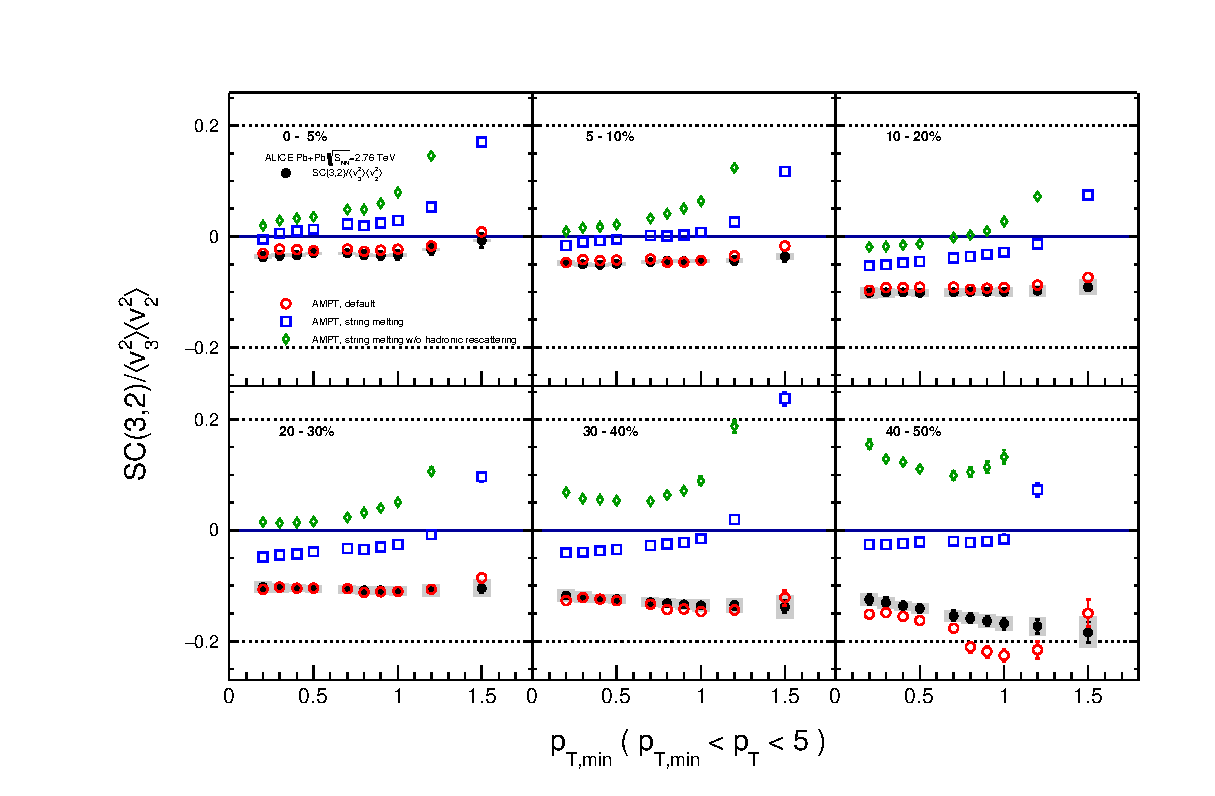
\includegraphics{figs/fig5_QConly_xminpt_nSC32.eps}}
              \resizebox{0.95\textwidth}{!}{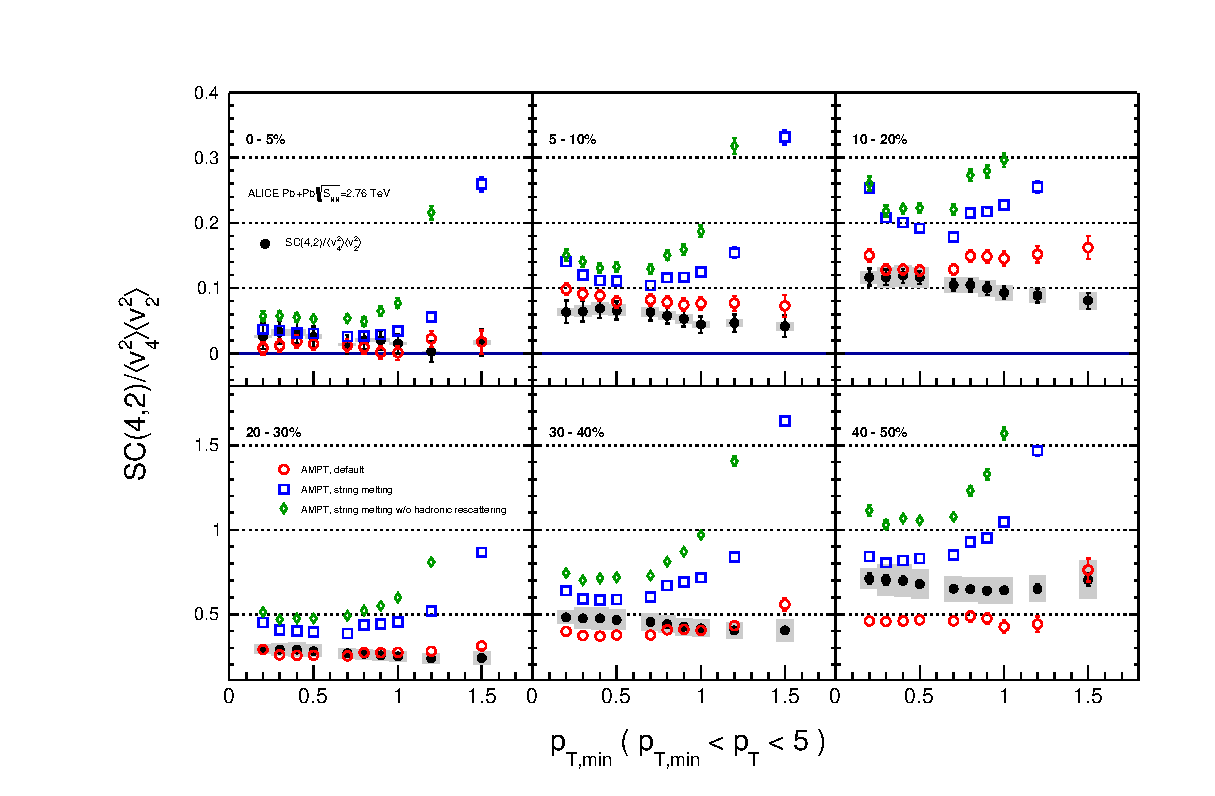
\includegraphics{figs/fig5_QConly_xminpt_nSC42.eps}}
              \end{center}
             \caption{NSC(3,2) (Top) and SC(4,2) (Bottom) as a function of minimum $p_{\rm T}$ cuts. The AMPT results are drawn as color bands for comparison. The details of the AMPT configurations can be found in Sec.~\ref{sec:models}.}
             \label{fig:Figure_8}
\end{figure}
  
\newpage
\section{Summary}
\label{sec:summary}
In summary, we have measured the Symmetric 2-harmonic 4-particle Cumulants (SC), which quantify the relationship between event-by-event fluctuations of two different flow harmonics. The observables are particularly robust against few-particle non-flow correlations and they provide orthogonal information to recently analysed symmetry plane correlators. We have found that fluctuations of $v_2$ and $v_3$ ($v_3$ and $v_4$) are anti-correlated in all centralities and fluctuations of $v_2$ and $v_4$ ( $v_2$ and $v_5$, $v_3$ and $v_5$) are correlated for all centralities. 
This feature was explored to discriminate between various hydro model calculations with different initial conditions as well as different parametrizations of the temperature dependence of $\eta/s$.
We have found that the different order harmonic correlations have different sensitivities to the initial conditions and the system properties. Therefore they have discriminating power on separating the role of the $\eta/s$  from the initial condition to the final state particle anisotropies.
Furthermore, the sign of $v_3$-$v_2$ correlation in the model in 0-10\% central collisions was found to be different between the data and hydrodynamic model calculations.
In the most central collisions the anisotropies originate mainly from fluctuations, i.e.\ the initial ellipsoidal geometry characteristic for mid-central collisions plays little role in this regime. Hence this observation might help to understand the details of the fluctuations in initial conditions. 
The comparisons to VISH2+1 calculation show that all the models with the large share viscosity regardless of the initial conditions failed to capture the centrality dependence of higher order correlations, more clearly than lower order harmonic correlations and based on the tested model parameters that the $\eta/s$ should be small and AMPT initial condition is flavored by the data. A quite clear separation of the correlation strength between different initial conditions is observed for these higher order harmonic correlations compared to the lower order harmonic correlations.
Finally we have found that $v_3$-$v_2$ and $v_4$-$v_2$ correlations have moderate $p_{\rm T}$ dependence in mid central collisions. This might be an indication of possible viscous corrections for the equilibrium distribution at hadronic freeze-out.
The results presented in this article can be used to further optimize model parameters and put better constraints on the initial conditions and the transport properties in ultra-relativistic heavy-ion collisions.





%%%%%%%% acknowledgements
\newenvironment{acknowledgement}{\relax}{\relax}
\begin{acknowledgement}
\section*{Acknowledgements}
%The ALICE Collaboration would like to thank all its engineers and technicians for their invaluable contributions to the construction of the experiment and the CERN accelerator teams for the outstanding performance of the LHC complex.
%
The ALICE Collaboration gratefully acknowledges the resources and support provided by all Grid centres and the Worldwide LHC Computing Grid (WLCG) collaboration.
%
The ALICE Collaboration acknowledges the following funding agencies for their support in building and
running the ALICE detector:
%
State Committee of Science,  World Federation of Scientists (WFS)
and Swiss Fonds Kidagan, Armenia,
%
Conselho Nacional de Desenvolvimento Cient\'{\i}fico e Tecnol\'{o}gico (CNPq), Financiadora de Estudos e Projetos (FINEP),
Funda\c{c}\~{a}o de Amparo \`{a} Pesquisa do Estado de S\~{a}o Paulo (FAPESP);
%
National Natural Science Foundation of China (NSFC), the Chinese Ministry of Education (CMOE)
and the Ministry of Science and Technology of China (MSTC);
%
Ministry of Education and Youth of the Czech Republic;
%
Danish Natural Science Research Council, the Carlsberg Foundation and the Danish National Research Foundation;
%
The European Research Council under the European Community's Seventh Framework Programme;
%
Helsinki Institute of Physics and the Academy of Finland;
%
French CNRS-IN2P3, the `Region Pays de Loire', `Region Alsace', `Region Auvergne' and CEA, France;
%
German Bundesministerium fur Bildung, Wissenschaft, Forschung und Technologie (BMBF) and the Helmholtz Association;
%
General Secretariat for Research and Technology, Ministry of
Development, Greece;
%
Hungarian Orszagos Tudomanyos Kutatasi Alappgrammok (OTKA) and National Office for Research and Technology (NKTH);
%
Department of Atomic Energy and Department of Science and Technology of the Government of India;
%
Istituto Nazionale di Fisica Nucleare (INFN) and Centro Fermi -
Museo Storico della Fisica e Centro Studi e Ricerche "Enrico
Fermi", Italy;
%
MEXT Grant-in-Aid for Specially Promoted Research, Ja\-pan;
%
Joint Institute for Nuclear Research, Dubna;
%
National Research Foundation of Korea (NRF);
%
Consejo Nacional de Cienca y Tecnologia (CONACYT), Direccion General de Asuntos del Personal Academico(DGAPA), M\'{e}xico, :Amerique Latine Formation academique – European Commission(ALFA-EC) and the EPLANET Program
(European Particle Physics Latin American Network)
%
Stichting voor Fundamenteel Onderzoek der Materie (FOM) and the Nederlandse Organisatie voor Wetenschappelijk Onderzoek (NWO), Netherlands;
%
Research Council of Norway (NFR);
%
National Science Centre, Poland;
%
Ministry of National Education/Institute for Atomic Physics and Consiliul Naţional al Cercetării Ştiinţifice - Executive Agency for Higher Education Research Development and Innovation Funding (CNCS-UEFISCDI) - Romania;
%
Ministry of Education and Science of Russian Federation, Russian
Academy of Sciences, Russian Federal Agency of Atomic Energy,
Russian Federal Agency for Science and Innovations and The Russian
Foundation for Basic Research;
%
Ministry of Education of Slovakia;
%
Department of Science and Technology, South Africa;
%
Centro de Investigaciones Energeticas, Medioambientales y Tecnologicas (CIEMAT), E-Infrastructure shared between Europe and Latin America (EELA), Ministerio de Econom\'{i}a y Competitividad (MINECO) of Spain, Xunta de Galicia (Conseller\'{\i}a de Educaci\'{o}n),
Centro de Aplicaciones Tecnológicas y Desarrollo Nuclear (CEA\-DEN), Cubaenerg\'{\i}a, Cuba, and IAEA (International Atomic Energy Agency);
%
Swedish Research Council (VR) and Knut $\&$ Alice Wallenberg
Foundation (KAW);
%
Ukraine Ministry of Education and Science;
%
United Kingdom Science and Technology Facilities Council (STFC);
%
The United States Department of Energy, the United States National
Science Foundation, the State of Texas, and the State of Ohio;
%
Ministry of Science, Education and Sports of Croatia and  Unity through Knowledge Fund, Croatia.
%
Council of Scientific and Industrial Research (CSIR), New Delhi, India
    %%%%%%% get the lates version before submitting
\end{acknowledgement}
%
%
%%%%%%%% Bibliography (In case of using bibtex generate the bbl requested by arXiv)
%\bibliographystyle{apsrev4-1}   % Put here the style file name for the paper, i.e.apsrev4-1
%\bibliography{biblio}
%\input {bibliography.tex}  
%

% \bibliographystyle{mybibstyle}
%\bibliographystyle{utphys}
%\bibliography{paper}
\bibliographystyle{utphys}
\bibliography{paper}

\newpage
%
%\input{}               %%%%%%%%%%% put your appendices here
%
%%%%%%%%% appendix with author list
\appendix
\section{The ALICE Collaboration}
\label{app:collab}
%
% Collaboration: CERN-LHC-ALICE
% Generation Date is 2015/Feb/18

% How to use:
%%%%%%%%% appendix with author list
%\appendix
%\section{The ALICE Collaboration}
%\label{app:collab}
%\input{authors-list.tex}  %%%%%%% get the latest version before submitting

\begingroup
\small
\begin{flushleft}
J.~Adam\Irefn{org39}\And
D.~Adamov\'{a}\Irefn{org82}\And
M.M.~Aggarwal\Irefn{org86}\And
G.~Aglieri Rinella\Irefn{org36}\And
M.~Agnello\Irefn{org110}\And
N.~Agrawal\Irefn{org47}\And
Z.~Ahammed\Irefn{org130}\And
S.U.~Ahn\Irefn{org67}\And
I.~Aimo\Irefn{org93}\textsuperscript{,}\Irefn{org110}\And
S.~Aiola\Irefn{org135}\And
M.~Ajaz\Irefn{org16}\And
A.~Akindinov\Irefn{org57}\And
S.N.~Alam\Irefn{org130}\And
D.~Aleksandrov\Irefn{org99}\And
B.~Alessandro\Irefn{org110}\And
D.~Alexandre\Irefn{org101}\And
R.~Alfaro Molina\Irefn{org63}\And
A.~Alici\Irefn{org104}\textsuperscript{,}\Irefn{org12}\And
A.~Alkin\Irefn{org3}\And
J.~Alme\Irefn{org37}\And
T.~Alt\Irefn{org42}\And
S.~Altinpinar\Irefn{org18}\And
I.~Altsybeev\Irefn{org129}\And
C.~Alves Garcia Prado\Irefn{org118}\And
C.~Andrei\Irefn{org77}\And
A.~Andronic\Irefn{org96}\And
V.~Anguelov\Irefn{org92}\And
J.~Anielski\Irefn{org53}\And
T.~Anti\v{c}i\'{c}\Irefn{org97}\And
F.~Antinori\Irefn{org107}\And
P.~Antonioli\Irefn{org104}\And
L.~Aphecetche\Irefn{org112}\And
H.~Appelsh\"{a}user\Irefn{org52}\And
S.~Arcelli\Irefn{org28}\And
N.~Armesto\Irefn{org17}\And
R.~Arnaldi\Irefn{org110}\And
T.~Aronsson\Irefn{org135}\And
I.C.~Arsene\Irefn{org22}\And
M.~Arslandok\Irefn{org52}\And
A.~Augustinus\Irefn{org36}\And
R.~Averbeck\Irefn{org96}\And
M.D.~Azmi\Irefn{org19}\And
M.~Bach\Irefn{org42}\And
A.~Badal\`{a}\Irefn{org106}\And
Y.W.~Baek\Irefn{org43}\And
S.~Bagnasco\Irefn{org110}\And
R.~Bailhache\Irefn{org52}\And
R.~Bala\Irefn{org89}\And
A.~Baldisseri\Irefn{org15}\And
F.~Baltasar Dos Santos Pedrosa\Irefn{org36}\And
R.C.~Baral\Irefn{org60}\And
A.M.~Barbano\Irefn{org110}\And
R.~Barbera\Irefn{org29}\And
F.~Barile\Irefn{org33}\And
G.G.~Barnaf\"{o}ldi\Irefn{org134}\And
L.S.~Barnby\Irefn{org101}\And
V.~Barret\Irefn{org69}\And
P.~Bartalini\Irefn{org7}\And
J.~Bartke\Irefn{org115}\And
E.~Bartsch\Irefn{org52}\And
M.~Basile\Irefn{org28}\And
N.~Bastid\Irefn{org69}\And
S.~Basu\Irefn{org130}\And
B.~Bathen\Irefn{org53}\And
G.~Batigne\Irefn{org112}\And
A.~Batista Camejo\Irefn{org69}\And
B.~Batyunya\Irefn{org65}\And
P.C.~Batzing\Irefn{org22}\And
I.G.~Bearden\Irefn{org79}\And
H.~Beck\Irefn{org52}\And
C.~Bedda\Irefn{org110}\And
N.K.~Behera\Irefn{org48}\textsuperscript{,}\Irefn{org47}\And
I.~Belikov\Irefn{org54}\And
F.~Bellini\Irefn{org28}\And
H.~Bello Martinez\Irefn{org2}\And
R.~Bellwied\Irefn{org120}\And
R.~Belmont\Irefn{org133}\And
E.~Belmont-Moreno\Irefn{org63}\And
V.~Belyaev\Irefn{org75}\And
G.~Bencedi\Irefn{org134}\And
S.~Beole\Irefn{org27}\And
I.~Berceanu\Irefn{org77}\And
A.~Bercuci\Irefn{org77}\And
Y.~Berdnikov\Irefn{org84}\And
D.~Berenyi\Irefn{org134}\And
R.A.~Bertens\Irefn{org56}\And
D.~Berzano\Irefn{org36}\textsuperscript{,}\Irefn{org27}\And
L.~Betev\Irefn{org36}\And
A.~Bhasin\Irefn{org89}\And
I.R.~Bhat\Irefn{org89}\And
A.K.~Bhati\Irefn{org86}\And
B.~Bhattacharjee\Irefn{org44}\And
J.~Bhom\Irefn{org126}\And
L.~Bianchi\Irefn{org27}\textsuperscript{,}\Irefn{org120}\And
N.~Bianchi\Irefn{org71}\And
C.~Bianchin\Irefn{org133}\textsuperscript{,}\Irefn{org56}\And
J.~Biel\v{c}\'{\i}k\Irefn{org39}\And
J.~Biel\v{c}\'{\i}kov\'{a}\Irefn{org82}\And
A.~Bilandzic\Irefn{org79}\And
S.~Biswas\Irefn{org78}\And
S.~Bjelogrlic\Irefn{org56}\And
F.~Blanco\Irefn{org10}\And
D.~Blau\Irefn{org99}\And
C.~Blume\Irefn{org52}\And
F.~Bock\Irefn{org73}\textsuperscript{,}\Irefn{org92}\And
A.~Bogdanov\Irefn{org75}\And
H.~B{\o}ggild\Irefn{org79}\And
L.~Boldizs\'{a}r\Irefn{org134}\And
M.~Bombara\Irefn{org40}\And
J.~Book\Irefn{org52}\And
H.~Borel\Irefn{org15}\And
A.~Borissov\Irefn{org95}\And
M.~Borri\Irefn{org81}\And
F.~Boss\'u\Irefn{org64}\And
M.~Botje\Irefn{org80}\And
E.~Botta\Irefn{org27}\And
S.~B\"{o}ttger\Irefn{org51}\And
P.~Braun-Munzinger\Irefn{org96}\And
M.~Bregant\Irefn{org118}\And
T.~Breitner\Irefn{org51}\And
T.A.~Broker\Irefn{org52}\And
T.A.~Browning\Irefn{org94}\And
M.~Broz\Irefn{org39}\And
E.J.~Brucken\Irefn{org45}\And
E.~Bruna\Irefn{org110}\And
G.E.~Bruno\Irefn{org33}\And
D.~Budnikov\Irefn{org98}\And
H.~Buesching\Irefn{org52}\And
S.~Bufalino\Irefn{org110}\textsuperscript{,}\Irefn{org36}\And
P.~Buncic\Irefn{org36}\And
O.~Busch\Irefn{org92}\textsuperscript{,}\Irefn{org126}\And
Z.~Buthelezi\Irefn{org64}\And
J.T.~Buxton\Irefn{org20}\And
D.~Caffarri\Irefn{org36}\textsuperscript{,}\Irefn{org30}\And
X.~Cai\Irefn{org7}\And
H.~Caines\Irefn{org135}\And
L.~Calero Diaz\Irefn{org71}\And
A.~Caliva\Irefn{org56}\And
E.~Calvo Villar\Irefn{org102}\And
P.~Camerini\Irefn{org26}\And
F.~Carena\Irefn{org36}\And
W.~Carena\Irefn{org36}\And
J.~Castillo Castellanos\Irefn{org15}\And
A.J.~Castro\Irefn{org123}\And
E.A.R.~Casula\Irefn{org25}\And
C.~Cavicchioli\Irefn{org36}\And
C.~Ceballos Sanchez\Irefn{org9}\And
J.~Cepila\Irefn{org39}\And
P.~Cerello\Irefn{org110}\And
B.~Chang\Irefn{org121}\And
S.~Chapeland\Irefn{org36}\And
M.~Chartier\Irefn{org122}\And
J.L.~Charvet\Irefn{org15}\And
S.~Chattopadhyay\Irefn{org130}\And
S.~Chattopadhyay\Irefn{org100}\And
V.~Chelnokov\Irefn{org3}\And
M.~Cherney\Irefn{org85}\And
C.~Cheshkov\Irefn{org128}\And
B.~Cheynis\Irefn{org128}\And
V.~Chibante Barroso\Irefn{org36}\And
D.D.~Chinellato\Irefn{org119}\And
P.~Chochula\Irefn{org36}\And
K.~Choi\Irefn{org95}\And
M.~Chojnacki\Irefn{org79}\And
S.~Choudhury\Irefn{org130}\And
P.~Christakoglou\Irefn{org80}\And
C.H.~Christensen\Irefn{org79}\And
P.~Christiansen\Irefn{org34}\And
T.~Chujo\Irefn{org126}\And
S.U.~Chung\Irefn{org95}\And
Z.~Chunhui\Irefn{org56}\And
C.~Cicalo\Irefn{org105}\And
L.~Cifarelli\Irefn{org12}\textsuperscript{,}\Irefn{org28}\And
F.~Cindolo\Irefn{org104}\And
J.~Cleymans\Irefn{org88}\And
F.~Colamaria\Irefn{org33}\And
D.~Colella\Irefn{org33}\And
A.~Collu\Irefn{org25}\And
M.~Colocci\Irefn{org28}\And
G.~Conesa Balbastre\Irefn{org70}\And
Z.~Conesa del Valle\Irefn{org50}\And
M.E.~Connors\Irefn{org135}\And
J.G.~Contreras\Irefn{org39}\textsuperscript{,}\Irefn{org11}\And
T.M.~Cormier\Irefn{org83}\And
Y.~Corrales Morales\Irefn{org27}\And
I.~Cort\'{e}s Maldonado\Irefn{org2}\And
P.~Cortese\Irefn{org32}\And
M.R.~Cosentino\Irefn{org118}\And
F.~Costa\Irefn{org36}\And
P.~Crochet\Irefn{org69}\And
R.~Cruz Albino\Irefn{org11}\And
E.~Cuautle\Irefn{org62}\And
L.~Cunqueiro\Irefn{org36}\And
T.~Dahms\Irefn{org91}\And
A.~Dainese\Irefn{org107}\And
A.~Danu\Irefn{org61}\And
D.~Das\Irefn{org100}\And
I.~Das\Irefn{org100}\textsuperscript{,}\Irefn{org50}\And
S.~Das\Irefn{org4}\And
A.~Dash\Irefn{org119}\And
S.~Dash\Irefn{org47}\And
S.~De\Irefn{org118}\And
A.~De Caro\Irefn{org31}\textsuperscript{,}\Irefn{org12}\And
G.~de Cataldo\Irefn{org103}\And
J.~de Cuveland\Irefn{org42}\And
A.~De Falco\Irefn{org25}\And
D.~De Gruttola\Irefn{org12}\textsuperscript{,}\Irefn{org31}\And
N.~De Marco\Irefn{org110}\And
S.~De Pasquale\Irefn{org31}\And
A.~Deisting\Irefn{org96}\textsuperscript{,}\Irefn{org92}\And
A.~Deloff\Irefn{org76}\And
E.~D\'{e}nes\Irefn{org134}\And
G.~D'Erasmo\Irefn{org33}\And
D.~Di Bari\Irefn{org33}\And
A.~Di Mauro\Irefn{org36}\And
P.~Di Nezza\Irefn{org71}\And
M.A.~Diaz Corchero\Irefn{org10}\And
T.~Dietel\Irefn{org88}\And
P.~Dillenseger\Irefn{org52}\And
R.~Divi\`{a}\Irefn{org36}\And
{\O}.~Djuvsland\Irefn{org18}\And
A.~Dobrin\Irefn{org56}\textsuperscript{,}\Irefn{org80}\And
T.~Dobrowolski\Irefn{org76}\Aref{0}\And
D.~Domenicis Gimenez\Irefn{org118}\And
B.~D\"{o}nigus\Irefn{org52}\And
O.~Dordic\Irefn{org22}\And
A.K.~Dubey\Irefn{org130}\And
A.~Dubla\Irefn{org56}\And
L.~Ducroux\Irefn{org128}\And
P.~Dupieux\Irefn{org69}\And
R.J.~Ehlers\Irefn{org135}\And
D.~Elia\Irefn{org103}\And
H.~Engel\Irefn{org51}\And
B.~Erazmus\Irefn{org112}\textsuperscript{,}\Irefn{org36}\And
F.~Erhardt\Irefn{org127}\And
D.~Eschweiler\Irefn{org42}\And
B.~Espagnon\Irefn{org50}\And
M.~Estienne\Irefn{org112}\And
S.~Esumi\Irefn{org126}\And
J.~Eum\Irefn{org95}\And
D.~Evans\Irefn{org101}\And
S.~Evdokimov\Irefn{org111}\And
G.~Eyyubova\Irefn{org39}\And
L.~Fabbietti\Irefn{org91}\And
D.~Fabris\Irefn{org107}\And
J.~Faivre\Irefn{org70}\And
A.~Fantoni\Irefn{org71}\And
M.~Fasel\Irefn{org73}\And
L.~Feldkamp\Irefn{org53}\And
D.~Felea\Irefn{org61}\And
A.~Feliciello\Irefn{org110}\And
G.~Feofilov\Irefn{org129}\And
J.~Ferencei\Irefn{org82}\And
A.~Fern\'{a}ndez T\'{e}llez\Irefn{org2}\And
E.G.~Ferreiro\Irefn{org17}\And
A.~Ferretti\Irefn{org27}\And
A.~Festanti\Irefn{org30}\And
J.~Figiel\Irefn{org115}\And
M.A.S.~Figueredo\Irefn{org122}\And
S.~Filchagin\Irefn{org98}\And
D.~Finogeev\Irefn{org55}\And
F.M.~Fionda\Irefn{org103}\And
E.M.~Fiore\Irefn{org33}\And
M.G.~Fleck\Irefn{org92}\And
M.~Floris\Irefn{org36}\And
S.~Foertsch\Irefn{org64}\And
P.~Foka\Irefn{org96}\And
S.~Fokin\Irefn{org99}\And
E.~Fragiacomo\Irefn{org109}\And
A.~Francescon\Irefn{org36}\textsuperscript{,}\Irefn{org30}\And
U.~Frankenfeld\Irefn{org96}\And
U.~Fuchs\Irefn{org36}\And
C.~Furget\Irefn{org70}\And
A.~Furs\Irefn{org55}\And
M.~Fusco Girard\Irefn{org31}\And
J.J.~Gaardh{\o}je\Irefn{org79}\And
M.~Gagliardi\Irefn{org27}\And
A.M.~Gago\Irefn{org102}\And
M.~Gallio\Irefn{org27}\And
D.R.~Gangadharan\Irefn{org73}\And
P.~Ganoti\Irefn{org87}\And
C.~Gao\Irefn{org7}\And
C.~Garabatos\Irefn{org96}\And
E.~Garcia-Solis\Irefn{org13}\And
C.~Gargiulo\Irefn{org36}\And
P.~Gasik\Irefn{org91}\And
M.~Germain\Irefn{org112}\And
A.~Gheata\Irefn{org36}\And
M.~Gheata\Irefn{org61}\textsuperscript{,}\Irefn{org36}\And
P.~Ghosh\Irefn{org130}\And
S.K.~Ghosh\Irefn{org4}\And
P.~Gianotti\Irefn{org71}\And
P.~Giubellino\Irefn{org36}\And
P.~Giubilato\Irefn{org30}\And
E.~Gladysz-Dziadus\Irefn{org115}\And
P.~Gl\"{a}ssel\Irefn{org92}\And
A.~Gomez Ramirez\Irefn{org51}\And
P.~Gonz\'{a}lez-Zamora\Irefn{org10}\And
S.~Gorbunov\Irefn{org42}\And
L.~G\"{o}rlich\Irefn{org115}\And
S.~Gotovac\Irefn{org114}\And
V.~Grabski\Irefn{org63}\And
L.K.~Graczykowski\Irefn{org132}\And
A.~Grelli\Irefn{org56}\And
A.~Grigoras\Irefn{org36}\And
C.~Grigoras\Irefn{org36}\And
V.~Grigoriev\Irefn{org75}\And
A.~Grigoryan\Irefn{org1}\And
S.~Grigoryan\Irefn{org65}\And
B.~Grinyov\Irefn{org3}\And
N.~Grion\Irefn{org109}\And
J.F.~Grosse-Oetringhaus\Irefn{org36}\And
J.-Y.~Grossiord\Irefn{org128}\And
R.~Grosso\Irefn{org36}\And
F.~Guber\Irefn{org55}\And
R.~Guernane\Irefn{org70}\And
B.~Guerzoni\Irefn{org28}\And
K.~Gulbrandsen\Irefn{org79}\And
H.~Gulkanyan\Irefn{org1}\And
T.~Gunji\Irefn{org125}\And
A.~Gupta\Irefn{org89}\And
R.~Gupta\Irefn{org89}\And
R.~Haake\Irefn{org53}\And
{\O}.~Haaland\Irefn{org18}\And
C.~Hadjidakis\Irefn{org50}\And
M.~Haiduc\Irefn{org61}\And
H.~Hamagaki\Irefn{org125}\And
G.~Hamar\Irefn{org134}\And
L.D.~Hanratty\Irefn{org101}\And
A.~Hansen\Irefn{org79}\And
J.W.~Harris\Irefn{org135}\And
H.~Hartmann\Irefn{org42}\And
A.~Harton\Irefn{org13}\And
D.~Hatzifotiadou\Irefn{org104}\And
S.~Hayashi\Irefn{org125}\And
S.T.~Heckel\Irefn{org52}\And
M.~Heide\Irefn{org53}\And
H.~Helstrup\Irefn{org37}\And
A.~Herghelegiu\Irefn{org77}\And
G.~Herrera Corral\Irefn{org11}\And
B.A.~Hess\Irefn{org35}\And
K.F.~Hetland\Irefn{org37}\And
T.E.~Hilden\Irefn{org45}\And
H.~Hillemanns\Irefn{org36}\And
B.~Hippolyte\Irefn{org54}\And
P.~Hristov\Irefn{org36}\And
M.~Huang\Irefn{org18}\And
T.J.~Humanic\Irefn{org20}\And
N.~Hussain\Irefn{org44}\And
T.~Hussain\Irefn{org19}\And
D.~Hutter\Irefn{org42}\And
D.S.~Hwang\Irefn{org21}\And
R.~Ilkaev\Irefn{org98}\And
I.~Ilkiv\Irefn{org76}\And
M.~Inaba\Irefn{org126}\And
C.~Ionita\Irefn{org36}\And
M.~Ippolitov\Irefn{org75}\textsuperscript{,}\Irefn{org99}\And
M.~Irfan\Irefn{org19}\And
M.~Ivanov\Irefn{org96}\And
V.~Ivanov\Irefn{org84}\And
V.~Izucheev\Irefn{org111}\And
P.M.~Jacobs\Irefn{org73}\And
C.~Jahnke\Irefn{org118}\And
H.J.~Jang\Irefn{org67}\And
M.A.~Janik\Irefn{org132}\And
P.H.S.Y.~Jayarathna\Irefn{org120}\And
C.~Jena\Irefn{org30}\And
S.~Jena\Irefn{org120}\And
R.T.~Jimenez Bustamante\Irefn{org62}\And
P.G.~Jones\Irefn{org101}\And
H.~Jung\Irefn{org43}\And
A.~Jusko\Irefn{org101}\And
P.~Kalinak\Irefn{org58}\And
A.~Kalweit\Irefn{org36}\And
J.~Kamin\Irefn{org52}\And
J.H.~Kang\Irefn{org136}\And
V.~Kaplin\Irefn{org75}\And
S.~Kar\Irefn{org130}\And
A.~Karasu Uysal\Irefn{org68}\And
O.~Karavichev\Irefn{org55}\And
T.~Karavicheva\Irefn{org55}\And
E.~Karpechev\Irefn{org55}\And
U.~Kebschull\Irefn{org51}\And
R.~Keidel\Irefn{org137}\And
D.L.D.~Keijdener\Irefn{org56}\And
M.~Keil\Irefn{org36}\And
K.H.~Khan\Irefn{org16}\And
M.M.~Khan\Irefn{org19}\And
P.~Khan\Irefn{org100}\And
S.A.~Khan\Irefn{org130}\And
A.~Khanzadeev\Irefn{org84}\And
Y.~Kharlov\Irefn{org111}\And
B.~Kileng\Irefn{org37}\And
B.~Kim\Irefn{org136}\And
D.W.~Kim\Irefn{org43}\textsuperscript{,}\Irefn{org67}\And
D.J.~Kim\Irefn{org121}\And
H.~Kim\Irefn{org136}\And
J.S.~Kim\Irefn{org43}\And
M.~Kim\Irefn{org43}\And
M.~Kim\Irefn{org136}\And
S.~Kim\Irefn{org21}\And
T.~Kim\Irefn{org136}\And
S.~Kirsch\Irefn{org42}\And
I.~Kisel\Irefn{org42}\And
S.~Kiselev\Irefn{org57}\And
A.~Kisiel\Irefn{org132}\And
G.~Kiss\Irefn{org134}\And
J.L.~Klay\Irefn{org6}\And
C.~Klein\Irefn{org52}\And
J.~Klein\Irefn{org92}\And
C.~Klein-B\"{o}sing\Irefn{org53}\And
A.~Kluge\Irefn{org36}\And
M.L.~Knichel\Irefn{org92}\And
A.G.~Knospe\Irefn{org116}\And
T.~Kobayashi\Irefn{org126}\And
C.~Kobdaj\Irefn{org113}\And
M.~Kofarago\Irefn{org36}\And
M.K.~K\"{o}hler\Irefn{org96}\And
T.~Kollegger\Irefn{org42}\textsuperscript{,}\Irefn{org96}\And
A.~Kolojvari\Irefn{org129}\And
V.~Kondratiev\Irefn{org129}\And
N.~Kondratyeva\Irefn{org75}\And
E.~Kondratyuk\Irefn{org111}\And
A.~Konevskikh\Irefn{org55}\And
C.~Kouzinopoulos\Irefn{org36}\And
O.~Kovalenko\Irefn{org76}\And
V.~Kovalenko\Irefn{org129}\And
M.~Kowalski\Irefn{org36}\textsuperscript{,}\Irefn{org115}\And
S.~Kox\Irefn{org70}\And
G.~Koyithatta Meethaleveedu\Irefn{org47}\And
J.~Kral\Irefn{org121}\And
I.~Kr\'{a}lik\Irefn{org58}\And
A.~Krav\v{c}\'{a}kov\'{a}\Irefn{org40}\And
M.~Krelina\Irefn{org39}\And
M.~Kretz\Irefn{org42}\And
M.~Krivda\Irefn{org101}\textsuperscript{,}\Irefn{org58}\And
F.~Krizek\Irefn{org82}\And
E.~Kryshen\Irefn{org36}\And
M.~Krzewicki\Irefn{org96}\textsuperscript{,}\Irefn{org42}\And
A.M.~Kubera\Irefn{org20}\And
V.~Ku\v{c}era\Irefn{org82}\And
T.~Kugathasan\Irefn{org36}\And
C.~Kuhn\Irefn{org54}\And
P.G.~Kuijer\Irefn{org80}\And
I.~Kulakov\Irefn{org42}\And
J.~Kumar\Irefn{org47}\And
L.~Kumar\Irefn{org78}\textsuperscript{,}\Irefn{org86}\And
P.~Kurashvili\Irefn{org76}\And
A.~Kurepin\Irefn{org55}\And
A.B.~Kurepin\Irefn{org55}\And
A.~Kuryakin\Irefn{org98}\And
S.~Kushpil\Irefn{org82}\And
M.J.~Kweon\Irefn{org49}\And
Y.~Kwon\Irefn{org136}\And
S.L.~La Pointe\Irefn{org110}\And
P.~La Rocca\Irefn{org29}\And
C.~Lagana Fernandes\Irefn{org118}\And
I.~Lakomov\Irefn{org36}\textsuperscript{,}\Irefn{org50}\And
R.~Langoy\Irefn{org41}\And
C.~Lara\Irefn{org51}\And
A.~Lardeux\Irefn{org15}\And
A.~Lattuca\Irefn{org27}\And
E.~Laudi\Irefn{org36}\And
R.~Lea\Irefn{org26}\And
L.~Leardini\Irefn{org92}\And
G.R.~Lee\Irefn{org101}\And
S.~Lee\Irefn{org136}\And
I.~Legrand\Irefn{org36}\And
R.C.~Lemmon\Irefn{org81}\And
V.~Lenti\Irefn{org103}\And
E.~Leogrande\Irefn{org56}\And
I.~Le\'{o}n Monz\'{o}n\Irefn{org117}\And
M.~Leoncino\Irefn{org27}\And
P.~L\'{e}vai\Irefn{org134}\And
S.~Li\Irefn{org7}\textsuperscript{,}\Irefn{org69}\And
X.~Li\Irefn{org14}\And
J.~Lien\Irefn{org41}\And
R.~Lietava\Irefn{org101}\And
S.~Lindal\Irefn{org22}\And
V.~Lindenstruth\Irefn{org42}\And
C.~Lippmann\Irefn{org96}\And
M.A.~Lisa\Irefn{org20}\And
H.M.~Ljunggren\Irefn{org34}\And
D.F.~Lodato\Irefn{org56}\And
P.I.~Loenne\Irefn{org18}\And
V.R.~Loggins\Irefn{org133}\And
V.~Loginov\Irefn{org75}\And
C.~Loizides\Irefn{org73}\And
X.~Lopez\Irefn{org69}\And
E.~L\'{o}pez Torres\Irefn{org9}\And
A.~Lowe\Irefn{org134}\And
P.~Luettig\Irefn{org52}\And
M.~Lunardon\Irefn{org30}\And
G.~Luparello\Irefn{org26}\textsuperscript{,}\Irefn{org56}\And
P.H.F.N.D.~Luz\Irefn{org118}\And
A.~Maevskaya\Irefn{org55}\And
M.~Mager\Irefn{org36}\And
S.~Mahajan\Irefn{org89}\And
S.M.~Mahmood\Irefn{org22}\And
A.~Maire\Irefn{org54}\And
R.D.~Majka\Irefn{org135}\And
M.~Malaev\Irefn{org84}\And
I.~Maldonado Cervantes\Irefn{org62}\And
L.~Malinina\Irefn{org65}\And
D.~Mal'Kevich\Irefn{org57}\And
P.~Malzacher\Irefn{org96}\And
A.~Mamonov\Irefn{org98}\And
L.~Manceau\Irefn{org110}\And
V.~Manko\Irefn{org99}\And
F.~Manso\Irefn{org69}\And
V.~Manzari\Irefn{org103}\textsuperscript{,}\Irefn{org36}\And
M.~Marchisone\Irefn{org27}\And
J.~Mare\v{s}\Irefn{org59}\And
G.V.~Margagliotti\Irefn{org26}\And
A.~Margotti\Irefn{org104}\And
J.~Margutti\Irefn{org56}\And
A.~Mar\'{\i}n\Irefn{org96}\And
C.~Markert\Irefn{org116}\And
M.~Marquard\Irefn{org52}\And
N.A.~Martin\Irefn{org96}\And
J.~Martin Blanco\Irefn{org112}\And
P.~Martinengo\Irefn{org36}\And
M.I.~Mart\'{\i}nez\Irefn{org2}\And
G.~Mart\'{\i}nez Garc\'{\i}a\Irefn{org112}\And
M.~Martinez Pedreira\Irefn{org36}\And
Y.~Martynov\Irefn{org3}\And
A.~Mas\Irefn{org118}\And
S.~Masciocchi\Irefn{org96}\And
M.~Masera\Irefn{org27}\And
A.~Masoni\Irefn{org105}\And
L.~Massacrier\Irefn{org112}\And
A.~Mastroserio\Irefn{org33}\And
H.~Masui\Irefn{org126}\And
A.~Matyja\Irefn{org115}\And
C.~Mayer\Irefn{org115}\And
J.~Mazer\Irefn{org123}\And
M.A.~Mazzoni\Irefn{org108}\And
D.~Mcdonald\Irefn{org120}\And
F.~Meddi\Irefn{org24}\And
A.~Menchaca-Rocha\Irefn{org63}\And
E.~Meninno\Irefn{org31}\And
J.~Mercado P\'erez\Irefn{org92}\And
M.~Meres\Irefn{org38}\And
Y.~Miake\Irefn{org126}\And
M.M.~Mieskolainen\Irefn{org45}\And
K.~Mikhaylov\Irefn{org57}\textsuperscript{,}\Irefn{org65}\And
L.~Milano\Irefn{org36}\And
J.~Milosevic\Irefn{org22}\textsuperscript{,}\Irefn{org131}\And
L.M.~Minervini\Irefn{org103}\textsuperscript{,}\Irefn{org23}\And
A.~Mischke\Irefn{org56}\And
A.N.~Mishra\Irefn{org48}\And
D.~Mi\'{s}kowiec\Irefn{org96}\And
J.~Mitra\Irefn{org130}\And
C.M.~Mitu\Irefn{org61}\And
N.~Mohammadi\Irefn{org56}\And
B.~Mohanty\Irefn{org130}\textsuperscript{,}\Irefn{org78}\And
L.~Molnar\Irefn{org54}\And
L.~Monta\~{n}o Zetina\Irefn{org11}\And
E.~Montes\Irefn{org10}\And
M.~Morando\Irefn{org30}\And
D.A.~Moreira De Godoy\Irefn{org112}\And
S.~Moretto\Irefn{org30}\And
A.~Morreale\Irefn{org112}\And
A.~Morsch\Irefn{org36}\And
V.~Muccifora\Irefn{org71}\And
E.~Mudnic\Irefn{org114}\And
D.~M{\"u}hlheim\Irefn{org53}\And
S.~Muhuri\Irefn{org130}\And
M.~Mukherjee\Irefn{org130}\And
H.~M\"{u}ller\Irefn{org36}\And
J.D.~Mulligan\Irefn{org135}\And
M.G.~Munhoz\Irefn{org118}\And
S.~Murray\Irefn{org64}\And
L.~Musa\Irefn{org36}\And
J.~Musinsky\Irefn{org58}\And
B.K.~Nandi\Irefn{org47}\And
R.~Nania\Irefn{org104}\And
E.~Nappi\Irefn{org103}\And
M.U.~Naru\Irefn{org16}\And
C.~Nattrass\Irefn{org123}\And
K.~Nayak\Irefn{org78}\And
T.K.~Nayak\Irefn{org130}\And
S.~Nazarenko\Irefn{org98}\And
A.~Nedosekin\Irefn{org57}\And
L.~Nellen\Irefn{org62}\And
F.~Ng\Irefn{org120}\And
M.~Nicassio\Irefn{org96}\And
M.~Niculescu\Irefn{org61}\textsuperscript{,}\Irefn{org36}\And
J.~Niedziela\Irefn{org36}\And
B.S.~Nielsen\Irefn{org79}\And
S.~Nikolaev\Irefn{org99}\And
S.~Nikulin\Irefn{org99}\And
V.~Nikulin\Irefn{org84}\And
F.~Noferini\Irefn{org104}\textsuperscript{,}\Irefn{org12}\And
P.~Nomokonov\Irefn{org65}\And
G.~Nooren\Irefn{org56}\And
J.~Norman\Irefn{org122}\And
A.~Nyanin\Irefn{org99}\And
J.~Nystrand\Irefn{org18}\And
H.~Oeschler\Irefn{org92}\And
S.~Oh\Irefn{org135}\And
S.K.~Oh\Irefn{org66}\And
A.~Ohlson\Irefn{org36}\And
A.~Okatan\Irefn{org68}\And
T.~Okubo\Irefn{org46}\And
L.~Olah\Irefn{org134}\And
J.~Oleniacz\Irefn{org132}\And
A.C.~Oliveira Da Silva\Irefn{org118}\And
M.H.~Oliver\Irefn{org135}\And
J.~Onderwaater\Irefn{org96}\And
C.~Oppedisano\Irefn{org110}\And
A.~Ortiz Velasquez\Irefn{org62}\And
A.~Oskarsson\Irefn{org34}\And
J.~Otwinowski\Irefn{org96}\textsuperscript{,}\Irefn{org115}\And
K.~Oyama\Irefn{org92}\And
M.~Ozdemir\Irefn{org52}\And
Y.~Pachmayer\Irefn{org92}\And
P.~Pagano\Irefn{org31}\And
G.~Pai\'{c}\Irefn{org62}\And
C.~Pajares\Irefn{org17}\And
S.K.~Pal\Irefn{org130}\And
J.~Pan\Irefn{org133}\And
A.K.~Pandey\Irefn{org47}\And
D.~Pant\Irefn{org47}\And
V.~Papikyan\Irefn{org1}\And
G.S.~Pappalardo\Irefn{org106}\And
P.~Pareek\Irefn{org48}\And
W.J.~Park\Irefn{org96}\And
S.~Parmar\Irefn{org86}\And
A.~Passfeld\Irefn{org53}\And
V.~Paticchio\Irefn{org103}\And
B.~Paul\Irefn{org100}\And
T.~Peitzmann\Irefn{org56}\And
H.~Pereira Da Costa\Irefn{org15}\And
E.~Pereira De Oliveira Filho\Irefn{org118}\And
D.~Peresunko\Irefn{org75}\textsuperscript{,}\Irefn{org99}\And
C.E.~P\'erez Lara\Irefn{org80}\And
V.~Peskov\Irefn{org52}\And
Y.~Pestov\Irefn{org5}\And
V.~Petr\'{a}\v{c}ek\Irefn{org39}\And
V.~Petrov\Irefn{org111}\And
M.~Petrovici\Irefn{org77}\And
C.~Petta\Irefn{org29}\And
S.~Piano\Irefn{org109}\And
M.~Pikna\Irefn{org38}\And
P.~Pillot\Irefn{org112}\And
O.~Pinazza\Irefn{org104}\textsuperscript{,}\Irefn{org36}\And
L.~Pinsky\Irefn{org120}\And
D.B.~Piyarathna\Irefn{org120}\And
M.~P\l osko\'{n}\Irefn{org73}\And
M.~Planinic\Irefn{org127}\And
J.~Pluta\Irefn{org132}\And
S.~Pochybova\Irefn{org134}\And
P.L.M.~Podesta-Lerma\Irefn{org117}\And
M.G.~Poghosyan\Irefn{org85}\And
B.~Polichtchouk\Irefn{org111}\And
N.~Poljak\Irefn{org127}\And
W.~Poonsawat\Irefn{org113}\And
A.~Pop\Irefn{org77}\And
S.~Porteboeuf-Houssais\Irefn{org69}\And
J.~Porter\Irefn{org73}\And
J.~Pospisil\Irefn{org82}\And
S.K.~Prasad\Irefn{org4}\And
R.~Preghenella\Irefn{org36}\textsuperscript{,}\Irefn{org104}\And
F.~Prino\Irefn{org110}\And
C.A.~Pruneau\Irefn{org133}\And
I.~Pshenichnov\Irefn{org55}\And
M.~Puccio\Irefn{org110}\And
G.~Puddu\Irefn{org25}\And
P.~Pujahari\Irefn{org133}\And
V.~Punin\Irefn{org98}\And
J.~Putschke\Irefn{org133}\And
H.~Qvigstad\Irefn{org22}\And
A.~Rachevski\Irefn{org109}\And
S.~Raha\Irefn{org4}\And
S.~Rajput\Irefn{org89}\And
J.~Rak\Irefn{org121}\And
A.~Rakotozafindrabe\Irefn{org15}\And
L.~Ramello\Irefn{org32}\And
R.~Raniwala\Irefn{org90}\And
S.~Raniwala\Irefn{org90}\And
S.S.~R\"{a}s\"{a}nen\Irefn{org45}\And
B.T.~Rascanu\Irefn{org52}\And
D.~Rathee\Irefn{org86}\And
K.F.~Read\Irefn{org123}\And
J.S.~Real\Irefn{org70}\And
K.~Redlich\Irefn{org76}\And
R.J.~Reed\Irefn{org133}\And
A.~Rehman\Irefn{org18}\And
P.~Reichelt\Irefn{org52}\And
M.~Reicher\Irefn{org56}\And
F.~Reidt\Irefn{org92}\textsuperscript{,}\Irefn{org36}\And
X.~Ren\Irefn{org7}\And
R.~Renfordt\Irefn{org52}\And
A.R.~Reolon\Irefn{org71}\And
A.~Reshetin\Irefn{org55}\And
F.~Rettig\Irefn{org42}\And
J.-P.~Revol\Irefn{org12}\And
K.~Reygers\Irefn{org92}\And
V.~Riabov\Irefn{org84}\And
R.A.~Ricci\Irefn{org72}\And
T.~Richert\Irefn{org34}\And
M.~Richter\Irefn{org22}\And
P.~Riedler\Irefn{org36}\And
W.~Riegler\Irefn{org36}\And
F.~Riggi\Irefn{org29}\And
C.~Ristea\Irefn{org61}\And
A.~Rivetti\Irefn{org110}\And
E.~Rocco\Irefn{org56}\And
M.~Rodr\'{i}guez Cahuantzi\Irefn{org11}\textsuperscript{,}\Irefn{org2}\And
A.~Rodriguez Manso\Irefn{org80}\And
K.~R{\o}ed\Irefn{org22}\And
E.~Rogochaya\Irefn{org65}\And
D.~Rohr\Irefn{org42}\And
D.~R\"ohrich\Irefn{org18}\And
R.~Romita\Irefn{org122}\And
F.~Ronchetti\Irefn{org71}\And
L.~Ronflette\Irefn{org112}\And
P.~Rosnet\Irefn{org69}\And
A.~Rossi\Irefn{org36}\And
F.~Roukoutakis\Irefn{org87}\And
A.~Roy\Irefn{org48}\And
C.~Roy\Irefn{org54}\And
P.~Roy\Irefn{org100}\And
A.J.~Rubio Montero\Irefn{org10}\And
R.~Rui\Irefn{org26}\And
R.~Russo\Irefn{org27}\And
E.~Ryabinkin\Irefn{org99}\And
Y.~Ryabov\Irefn{org84}\And
A.~Rybicki\Irefn{org115}\And
S.~Sadovsky\Irefn{org111}\And
K.~\v{S}afa\v{r}\'{\i}k\Irefn{org36}\And
B.~Sahlmuller\Irefn{org52}\And
P.~Sahoo\Irefn{org48}\And
R.~Sahoo\Irefn{org48}\And
S.~Sahoo\Irefn{org60}\And
P.K.~Sahu\Irefn{org60}\And
J.~Saini\Irefn{org130}\And
S.~Sakai\Irefn{org71}\And
M.A.~Saleh\Irefn{org133}\And
C.A.~Salgado\Irefn{org17}\And
J.~Salzwedel\Irefn{org20}\And
S.~Sambyal\Irefn{org89}\And
V.~Samsonov\Irefn{org84}\And
X.~Sanchez Castro\Irefn{org54}\And
L.~\v{S}\'{a}ndor\Irefn{org58}\And
A.~Sandoval\Irefn{org63}\And
M.~Sano\Irefn{org126}\And
G.~Santagati\Irefn{org29}\And
D.~Sarkar\Irefn{org130}\And
E.~Scapparone\Irefn{org104}\And
F.~Scarlassara\Irefn{org30}\And
R.P.~Scharenberg\Irefn{org94}\And
C.~Schiaua\Irefn{org77}\And
R.~Schicker\Irefn{org92}\And
C.~Schmidt\Irefn{org96}\And
H.R.~Schmidt\Irefn{org35}\And
S.~Schuchmann\Irefn{org52}\And
J.~Schukraft\Irefn{org36}\And
M.~Schulc\Irefn{org39}\And
T.~Schuster\Irefn{org135}\And
Y.~Schutz\Irefn{org112}\textsuperscript{,}\Irefn{org36}\And
K.~Schwarz\Irefn{org96}\And
K.~Schweda\Irefn{org96}\And
G.~Scioli\Irefn{org28}\And
E.~Scomparin\Irefn{org110}\And
R.~Scott\Irefn{org123}\And
K.S.~Seeder\Irefn{org118}\And
J.E.~Seger\Irefn{org85}\And
Y.~Sekiguchi\Irefn{org125}\And
I.~Selyuzhenkov\Irefn{org96}\And
K.~Senosi\Irefn{org64}\And
J.~Seo\Irefn{org66}\textsuperscript{,}\Irefn{org95}\And
E.~Serradilla\Irefn{org10}\textsuperscript{,}\Irefn{org63}\And
A.~Sevcenco\Irefn{org61}\And
A.~Shabanov\Irefn{org55}\And
A.~Shabetai\Irefn{org112}\And
O.~Shadura\Irefn{org3}\And
R.~Shahoyan\Irefn{org36}\And
A.~Shangaraev\Irefn{org111}\And
A.~Sharma\Irefn{org89}\And
N.~Sharma\Irefn{org60}\textsuperscript{,}\Irefn{org123}\And
K.~Shigaki\Irefn{org46}\And
K.~Shtejer\Irefn{org9}\textsuperscript{,}\Irefn{org27}\And
Y.~Sibiriak\Irefn{org99}\And
S.~Siddhanta\Irefn{org105}\And
K.M.~Sielewicz\Irefn{org36}\And
T.~Siemiarczuk\Irefn{org76}\And
D.~Silvermyr\Irefn{org83}\textsuperscript{,}\Irefn{org34}\And
C.~Silvestre\Irefn{org70}\And
G.~Simatovic\Irefn{org127}\And
G.~Simonetti\Irefn{org36}\And
R.~Singaraju\Irefn{org130}\And
R.~Singh\Irefn{org78}\And
S.~Singha\Irefn{org78}\textsuperscript{,}\Irefn{org130}\And
V.~Singhal\Irefn{org130}\And
B.C.~Sinha\Irefn{org130}\And
T.~Sinha\Irefn{org100}\And
B.~Sitar\Irefn{org38}\And
M.~Sitta\Irefn{org32}\And
T.B.~Skaali\Irefn{org22}\And
M.~Slupecki\Irefn{org121}\And
N.~Smirnov\Irefn{org135}\And
R.J.M.~Snellings\Irefn{org56}\And
T.W.~Snellman\Irefn{org121}\And
C.~S{\o}gaard\Irefn{org34}\And
R.~Soltz\Irefn{org74}\And
J.~Song\Irefn{org95}\And
M.~Song\Irefn{org136}\And
Z.~Song\Irefn{org7}\And
F.~Soramel\Irefn{org30}\And
S.~Sorensen\Irefn{org123}\And
M.~Spacek\Irefn{org39}\And
E.~Spiriti\Irefn{org71}\And
I.~Sputowska\Irefn{org115}\And
M.~Spyropoulou-Stassinaki\Irefn{org87}\And
B.K.~Srivastava\Irefn{org94}\And
J.~Stachel\Irefn{org92}\And
I.~Stan\Irefn{org61}\And
G.~Stefanek\Irefn{org76}\And
M.~Steinpreis\Irefn{org20}\And
E.~Stenlund\Irefn{org34}\And
G.~Steyn\Irefn{org64}\And
J.H.~Stiller\Irefn{org92}\And
D.~Stocco\Irefn{org112}\And
P.~Strmen\Irefn{org38}\And
A.A.P.~Suaide\Irefn{org118}\And
T.~Sugitate\Irefn{org46}\And
C.~Suire\Irefn{org50}\And
M.~Suleymanov\Irefn{org16}\And
R.~Sultanov\Irefn{org57}\And
M.~\v{S}umbera\Irefn{org82}\And
T.J.M.~Symons\Irefn{org73}\And
A.~Szabo\Irefn{org38}\And
A.~Szanto de Toledo\Irefn{org118}\And
I.~Szarka\Irefn{org38}\And
A.~Szczepankiewicz\Irefn{org36}\And
M.~Szymanski\Irefn{org132}\And
J.~Takahashi\Irefn{org119}\And
N.~Tanaka\Irefn{org126}\And
M.A.~Tangaro\Irefn{org33}\And
J.D.~Tapia Takaki\Aref{idp5842272}\textsuperscript{,}\Irefn{org50}\And
A.~Tarantola Peloni\Irefn{org52}\And
M.~Tariq\Irefn{org19}\And
M.G.~Tarzila\Irefn{org77}\And
A.~Tauro\Irefn{org36}\And
G.~Tejeda Mu\~{n}oz\Irefn{org2}\And
A.~Telesca\Irefn{org36}\And
K.~Terasaki\Irefn{org125}\And
C.~Terrevoli\Irefn{org30}\textsuperscript{,}\Irefn{org25}\And
B.~Teyssier\Irefn{org128}\And
J.~Th\"{a}der\Irefn{org96}\textsuperscript{,}\Irefn{org73}\And
D.~Thomas\Irefn{org116}\And
R.~Tieulent\Irefn{org128}\And
A.R.~Timmins\Irefn{org120}\And
A.~Toia\Irefn{org52}\And
S.~Trogolo\Irefn{org110}\And
V.~Trubnikov\Irefn{org3}\And
W.H.~Trzaska\Irefn{org121}\And
T.~Tsuji\Irefn{org125}\And
A.~Tumkin\Irefn{org98}\And
R.~Turrisi\Irefn{org107}\And
T.S.~Tveter\Irefn{org22}\And
K.~Ullaland\Irefn{org18}\And
A.~Uras\Irefn{org128}\And
G.L.~Usai\Irefn{org25}\And
A.~Utrobicic\Irefn{org127}\And
M.~Vajzer\Irefn{org82}\And
M.~Vala\Irefn{org58}\And
L.~Valencia Palomo\Irefn{org69}\And
S.~Vallero\Irefn{org27}\And
J.~Van Der Maarel\Irefn{org56}\And
J.W.~Van Hoorne\Irefn{org36}\And
M.~van Leeuwen\Irefn{org56}\And
T.~Vanat\Irefn{org82}\And
P.~Vande Vyvre\Irefn{org36}\And
D.~Varga\Irefn{org134}\And
A.~Vargas\Irefn{org2}\And
M.~Vargyas\Irefn{org121}\And
R.~Varma\Irefn{org47}\And
M.~Vasileiou\Irefn{org87}\And
A.~Vasiliev\Irefn{org99}\And
A.~Vauthier\Irefn{org70}\And
V.~Vechernin\Irefn{org129}\And
A.M.~Veen\Irefn{org56}\And
M.~Veldhoen\Irefn{org56}\And
A.~Velure\Irefn{org18}\And
M.~Venaruzzo\Irefn{org72}\And
E.~Vercellin\Irefn{org27}\And
S.~Vergara Lim\'on\Irefn{org2}\And
R.~Vernet\Irefn{org8}\And
M.~Verweij\Irefn{org133}\And
L.~Vickovic\Irefn{org114}\And
G.~Viesti\Irefn{org30}\Aref{0}\And
J.~Viinikainen\Irefn{org121}\And
Z.~Vilakazi\Irefn{org124}\And
O.~Villalobos Baillie\Irefn{org101}\And
A.~Vinogradov\Irefn{org99}\And
L.~Vinogradov\Irefn{org129}\And
Y.~Vinogradov\Irefn{org98}\And
T.~Virgili\Irefn{org31}\And
V.~Vislavicius\Irefn{org34}\And
Y.P.~Viyogi\Irefn{org130}\And
A.~Vodopyanov\Irefn{org65}\And
M.A.~V\"{o}lkl\Irefn{org92}\And
K.~Voloshin\Irefn{org57}\And
S.A.~Voloshin\Irefn{org133}\And
G.~Volpe\Irefn{org36}\textsuperscript{,}\Irefn{org134}\And
B.~von Haller\Irefn{org36}\And
I.~Vorobyev\Irefn{org91}\And
D.~Vranic\Irefn{org96}\textsuperscript{,}\Irefn{org36}\And
J.~Vrl\'{a}kov\'{a}\Irefn{org40}\And
B.~Vulpescu\Irefn{org69}\And
A.~Vyushin\Irefn{org98}\And
B.~Wagner\Irefn{org18}\And
J.~Wagner\Irefn{org96}\And
H.~Wang\Irefn{org56}\And
M.~Wang\Irefn{org7}\textsuperscript{,}\Irefn{org112}\And
Y.~Wang\Irefn{org92}\And
D.~Watanabe\Irefn{org126}\And
M.~Weber\Irefn{org36}\And
S.G.~Weber\Irefn{org96}\And
J.P.~Wessels\Irefn{org53}\And
U.~Westerhoff\Irefn{org53}\And
J.~Wiechula\Irefn{org35}\And
J.~Wikne\Irefn{org22}\And
M.~Wilde\Irefn{org53}\And
G.~Wilk\Irefn{org76}\And
J.~Wilkinson\Irefn{org92}\And
M.C.S.~Williams\Irefn{org104}\And
B.~Windelband\Irefn{org92}\And
M.~Winn\Irefn{org92}\And
C.G.~Yaldo\Irefn{org133}\And
Y.~Yamaguchi\Irefn{org125}\And
H.~Yang\Irefn{org56}\And
P.~Yang\Irefn{org7}\And
S.~Yano\Irefn{org46}\And
Z.~Yin\Irefn{org7}\And
H.~Yokoyama\Irefn{org126}\And
I.-K.~Yoo\Irefn{org95}\And
V.~Yurchenko\Irefn{org3}\And
I.~Yushmanov\Irefn{org99}\And
A.~Zaborowska\Irefn{org132}\And
V.~Zaccolo\Irefn{org79}\And
A.~Zaman\Irefn{org16}\And
C.~Zampolli\Irefn{org104}\And
H.J.C.~Zanoli\Irefn{org118}\And
S.~Zaporozhets\Irefn{org65}\And
A.~Zarochentsev\Irefn{org129}\And
P.~Z\'{a}vada\Irefn{org59}\And
N.~Zaviyalov\Irefn{org98}\And
H.~Zbroszczyk\Irefn{org132}\And
I.S.~Zgura\Irefn{org61}\And
M.~Zhalov\Irefn{org84}\And
H.~Zhang\Irefn{org7}\And
X.~Zhang\Irefn{org73}\And
Y.~Zhang\Irefn{org7}\And
C.~Zhao\Irefn{org22}\And
N.~Zhigareva\Irefn{org57}\And
D.~Zhou\Irefn{org7}\And
Y.~Zhou\Irefn{org56}\And
Z.~Zhou\Irefn{org18}\And
H.~Zhu\Irefn{org7}\And
J.~Zhu\Irefn{org7}\textsuperscript{,}\Irefn{org112}\And
X.~Zhu\Irefn{org7}\And
A.~Zichichi\Irefn{org12}\textsuperscript{,}\Irefn{org28}\And
A.~Zimmermann\Irefn{org92}\And
M.B.~Zimmermann\Irefn{org53}\textsuperscript{,}\Irefn{org36}\And
G.~Zinovjev\Irefn{org3}\And
M.~Zyzak\Irefn{org42}
\renewcommand\labelenumi{\textsuperscript{\theenumi}~}

\section*{Affiliation notes}
\renewcommand\theenumi{\roman{enumi}}
\begin{Authlist}
\item \Adef{0}Deceased
\item \Adef{idp5842272}{Also at: University of Kansas, Lawrence, Kansas, United States}
\end{Authlist}

\section*{Collaboration Institutes}
\renewcommand\theenumi{\arabic{enumi}~}
\begin{Authlist}

\item \Idef{org1}A.I. Alikhanyan National Science Laboratory (Yerevan Physics Institute) Foundation, Yerevan, Armenia
\item \Idef{org2}Benem\'{e}rita Universidad Aut\'{o}noma de Puebla, Puebla, Mexico
\item \Idef{org3}Bogolyubov Institute for Theoretical Physics, Kiev, Ukraine
\item \Idef{org4}Bose Institute, Department of Physics and Centre for Astroparticle Physics and Space Science (CAPSS), Kolkata, India
\item \Idef{org5}Budker Institute for Nuclear Physics, Novosibirsk, Russia
\item \Idef{org6}California Polytechnic State University, San Luis Obispo, California, United States
\item \Idef{org7}Central China Normal University, Wuhan, China
\item \Idef{org8}Centre de Calcul de l'IN2P3, Villeurbanne, France
\item \Idef{org9}Centro de Aplicaciones Tecnol\'{o}gicas y Desarrollo Nuclear (CEADEN), Havana, Cuba
\item \Idef{org10}Centro de Investigaciones Energ\'{e}ticas Medioambientales y Tecnol\'{o}gicas (CIEMAT), Madrid, Spain
\item \Idef{org11}Centro de Investigaci\'{o}n y de Estudios Avanzados (CINVESTAV), Mexico City and M\'{e}rida, Mexico
\item \Idef{org12}Centro Fermi - Museo Storico della Fisica e Centro Studi e Ricerche ``Enrico Fermi'', Rome, Italy
\item \Idef{org13}Chicago State University, Chicago, Illinois, USA
\item \Idef{org14}China Institute of Atomic Energy, Beijing, China
\item \Idef{org15}Commissariat \`{a} l'Energie Atomique, IRFU, Saclay, France
\item \Idef{org16}COMSATS Institute of Information Technology (CIIT), Islamabad, Pakistan
\item \Idef{org17}Departamento de F\'{\i}sica de Part\'{\i}culas and IGFAE, Universidad de Santiago de Compostela, Santiago de Compostela, Spain
\item \Idef{org18}Department of Physics and Technology, University of Bergen, Bergen, Norway
\item \Idef{org19}Department of Physics, Aligarh Muslim University, Aligarh, India
\item \Idef{org20}Department of Physics, Ohio State University, Columbus, Ohio, United States
\item \Idef{org21}Department of Physics, Sejong University, Seoul, South Korea
\item \Idef{org22}Department of Physics, University of Oslo, Oslo, Norway
\item \Idef{org23}Dipartimento di Elettrotecnica ed Elettronica del Politecnico, Bari, Italy
\item \Idef{org24}Dipartimento di Fisica dell'Universit\`{a} 'La Sapienza' and Sezione INFN Rome, Italy
\item \Idef{org25}Dipartimento di Fisica dell'Universit\`{a} and Sezione INFN, Cagliari, Italy
\item \Idef{org26}Dipartimento di Fisica dell'Universit\`{a} and Sezione INFN, Trieste, Italy
\item \Idef{org27}Dipartimento di Fisica dell'Universit\`{a} and Sezione INFN, Turin, Italy
\item \Idef{org28}Dipartimento di Fisica e Astronomia dell'Universit\`{a} and Sezione INFN, Bologna, Italy
\item \Idef{org29}Dipartimento di Fisica e Astronomia dell'Universit\`{a} and Sezione INFN, Catania, Italy
\item \Idef{org30}Dipartimento di Fisica e Astronomia dell'Universit\`{a} and Sezione INFN, Padova, Italy
\item \Idef{org31}Dipartimento di Fisica `E.R.~Caianiello' dell'Universit\`{a} and Gruppo Collegato INFN, Salerno, Italy
\item \Idef{org32}Dipartimento di Scienze e Innovazione Tecnologica dell'Universit\`{a} del  Piemonte Orientale and Gruppo Collegato INFN, Alessandria, Italy
\item \Idef{org33}Dipartimento Interateneo di Fisica `M.~Merlin' and Sezione INFN, Bari, Italy
\item \Idef{org34}Division of Experimental High Energy Physics, University of Lund, Lund, Sweden
\item \Idef{org35}Eberhard Karls Universit\"{a}t T\"{u}bingen, T\"{u}bingen, Germany
\item \Idef{org36}European Organization for Nuclear Research (CERN), Geneva, Switzerland
\item \Idef{org37}Faculty of Engineering, Bergen University College, Bergen, Norway
\item \Idef{org38}Faculty of Mathematics, Physics and Informatics, Comenius University, Bratislava, Slovakia
\item \Idef{org39}Faculty of Nuclear Sciences and Physical Engineering, Czech Technical University in Prague, Prague, Czech Republic
\item \Idef{org40}Faculty of Science, P.J.~\v{S}af\'{a}rik University, Ko\v{s}ice, Slovakia
\item \Idef{org41}Faculty of Technology, Buskerud and Vestfold University College, Vestfold, Norway
\item \Idef{org42}Frankfurt Institute for Advanced Studies, Johann Wolfgang Goethe-Universit\"{a}t Frankfurt, Frankfurt, Germany
\item \Idef{org43}Gangneung-Wonju National University, Gangneung, South Korea
\item \Idef{org44}Gauhati University, Department of Physics, Guwahati, India
\item \Idef{org45}Helsinki Institute of Physics (HIP), Helsinki, Finland
\item \Idef{org46}Hiroshima University, Hiroshima, Japan
\item \Idef{org47}Indian Institute of Technology Bombay (IIT), Mumbai, India
\item \Idef{org48}Indian Institute of Technology Indore, Indore (IITI), India
\item \Idef{org49}Inha University, Incheon, South Korea
\item \Idef{org50}Institut de Physique Nucl\'eaire d'Orsay (IPNO), Universit\'e Paris-Sud, CNRS-IN2P3, Orsay, France
\item \Idef{org51}Institut f\"{u}r Informatik, Johann Wolfgang Goethe-Universit\"{a}t Frankfurt, Frankfurt, Germany
\item \Idef{org52}Institut f\"{u}r Kernphysik, Johann Wolfgang Goethe-Universit\"{a}t Frankfurt, Frankfurt, Germany
\item \Idef{org53}Institut f\"{u}r Kernphysik, Westf\"{a}lische Wilhelms-Universit\"{a}t M\"{u}nster, M\"{u}nster, Germany
\item \Idef{org54}Institut Pluridisciplinaire Hubert Curien (IPHC), Universit\'{e} de Strasbourg, CNRS-IN2P3, Strasbourg, France
\item \Idef{org55}Institute for Nuclear Research, Academy of Sciences, Moscow, Russia
\item \Idef{org56}Institute for Subatomic Physics of Utrecht University, Utrecht, Netherlands
\item \Idef{org57}Institute for Theoretical and Experimental Physics, Moscow, Russia
\item \Idef{org58}Institute of Experimental Physics, Slovak Academy of Sciences, Ko\v{s}ice, Slovakia
\item \Idef{org59}Institute of Physics, Academy of Sciences of the Czech Republic, Prague, Czech Republic
\item \Idef{org60}Institute of Physics, Bhubaneswar, India
\item \Idef{org61}Institute of Space Science (ISS), Bucharest, Romania
\item \Idef{org62}Instituto de Ciencias Nucleares, Universidad Nacional Aut\'{o}noma de M\'{e}xico, Mexico City, Mexico
\item \Idef{org63}Instituto de F\'{\i}sica, Universidad Nacional Aut\'{o}noma de M\'{e}xico, Mexico City, Mexico
\item \Idef{org64}iThemba LABS, National Research Foundation, Somerset West, South Africa
\item \Idef{org65}Joint Institute for Nuclear Research (JINR), Dubna, Russia
\item \Idef{org66}Konkuk University, Seoul, South Korea
\item \Idef{org67}Korea Institute of Science and Technology Information, Daejeon, South Korea
\item \Idef{org68}KTO Karatay University, Konya, Turkey
\item \Idef{org69}Laboratoire de Physique Corpusculaire (LPC), Clermont Universit\'{e}, Universit\'{e} Blaise Pascal, CNRS--IN2P3, Clermont-Ferrand, France
\item \Idef{org70}Laboratoire de Physique Subatomique et de Cosmologie, Universit\'{e} Grenoble-Alpes, CNRS-IN2P3, Grenoble, France
\item \Idef{org71}Laboratori Nazionali di Frascati, INFN, Frascati, Italy
\item \Idef{org72}Laboratori Nazionali di Legnaro, INFN, Legnaro, Italy
\item \Idef{org73}Lawrence Berkeley National Laboratory, Berkeley, California, United States
\item \Idef{org74}Lawrence Livermore National Laboratory, Livermore, California, United States
\item \Idef{org75}Moscow Engineering Physics Institute, Moscow, Russia
\item \Idef{org76}National Centre for Nuclear Studies, Warsaw, Poland
\item \Idef{org77}National Institute for Physics and Nuclear Engineering, Bucharest, Romania
\item \Idef{org78}National Institute of Science Education and Research, Bhubaneswar, India
\item \Idef{org79}Niels Bohr Institute, University of Copenhagen, Copenhagen, Denmark
\item \Idef{org80}Nikhef, National Institute for Subatomic Physics, Amsterdam, Netherlands
\item \Idef{org81}Nuclear Physics Group, STFC Daresbury Laboratory, Daresbury, United Kingdom
\item \Idef{org82}Nuclear Physics Institute, Academy of Sciences of the Czech Republic, \v{R}e\v{z} u Prahy, Czech Republic
\item \Idef{org83}Oak Ridge National Laboratory, Oak Ridge, Tennessee, United States
\item \Idef{org84}Petersburg Nuclear Physics Institute, Gatchina, Russia
\item \Idef{org85}Physics Department, Creighton University, Omaha, Nebraska, United States
\item \Idef{org86}Physics Department, Panjab University, Chandigarh, India
\item \Idef{org87}Physics Department, University of Athens, Athens, Greece
\item \Idef{org88}Physics Department, University of Cape Town, Cape Town, South Africa
\item \Idef{org89}Physics Department, University of Jammu, Jammu, India
\item \Idef{org90}Physics Department, University of Rajasthan, Jaipur, India
\item \Idef{org91}Physik Department, Technische Universit\"{a}t M\"{u}nchen, Munich, Germany
\item \Idef{org92}Physikalisches Institut, Ruprecht-Karls-Universit\"{a}t Heidelberg, Heidelberg, Germany
\item \Idef{org93}Politecnico di Torino, Turin, Italy
\item \Idef{org94}Purdue University, West Lafayette, Indiana, United States
\item \Idef{org95}Pusan National University, Pusan, South Korea
\item \Idef{org96}Research Division and ExtreMe Matter Institute EMMI, GSI Helmholtzzentrum f\"ur Schwerionenforschung, Darmstadt, Germany
\item \Idef{org97}Rudjer Bo\v{s}kovi\'{c} Institute, Zagreb, Croatia
\item \Idef{org98}Russian Federal Nuclear Center (VNIIEF), Sarov, Russia
\item \Idef{org99}Russian Research Centre Kurchatov Institute, Moscow, Russia
\item \Idef{org100}Saha Institute of Nuclear Physics, Kolkata, India
\item \Idef{org101}School of Physics and Astronomy, University of Birmingham, Birmingham, United Kingdom
\item \Idef{org102}Secci\'{o}n F\'{\i}sica, Departamento de Ciencias, Pontificia Universidad Cat\'{o}lica del Per\'{u}, Lima, Peru
\item \Idef{org103}Sezione INFN, Bari, Italy
\item \Idef{org104}Sezione INFN, Bologna, Italy
\item \Idef{org105}Sezione INFN, Cagliari, Italy
\item \Idef{org106}Sezione INFN, Catania, Italy
\item \Idef{org107}Sezione INFN, Padova, Italy
\item \Idef{org108}Sezione INFN, Rome, Italy
\item \Idef{org109}Sezione INFN, Trieste, Italy
\item \Idef{org110}Sezione INFN, Turin, Italy
\item \Idef{org111}SSC IHEP of NRC Kurchatov institute, Protvino, Russia
\item \Idef{org112}SUBATECH, Ecole des Mines de Nantes, Universit\'{e} de Nantes, CNRS-IN2P3, Nantes, France
\item \Idef{org113}Suranaree University of Technology, Nakhon Ratchasima, Thailand
\item \Idef{org114}Technical University of Split FESB, Split, Croatia
\item \Idef{org115}The Henryk Niewodniczanski Institute of Nuclear Physics, Polish Academy of Sciences, Cracow, Poland
\item \Idef{org116}The University of Texas at Austin, Physics Department, Austin, Texas, USA
\item \Idef{org117}Universidad Aut\'{o}noma de Sinaloa, Culiac\'{a}n, Mexico
\item \Idef{org118}Universidade de S\~{a}o Paulo (USP), S\~{a}o Paulo, Brazil
\item \Idef{org119}Universidade Estadual de Campinas (UNICAMP), Campinas, Brazil
\item \Idef{org120}University of Houston, Houston, Texas, United States
\item \Idef{org121}University of Jyv\"{a}skyl\"{a}, Jyv\"{a}skyl\"{a}, Finland
\item \Idef{org122}University of Liverpool, Liverpool, United Kingdom
\item \Idef{org123}University of Tennessee, Knoxville, Tennessee, United States
\item \Idef{org124}University of the Witwatersrand, Johannesburg, South Africa
\item \Idef{org125}University of Tokyo, Tokyo, Japan
\item \Idef{org126}University of Tsukuba, Tsukuba, Japan
\item \Idef{org127}University of Zagreb, Zagreb, Croatia
\item \Idef{org128}Universit\'{e} de Lyon, Universit\'{e} Lyon 1, CNRS/IN2P3, IPN-Lyon, Villeurbanne, France
\item \Idef{org129}V.~Fock Institute for Physics, St. Petersburg State University, St. Petersburg, Russia
\item \Idef{org130}Variable Energy Cyclotron Centre, Kolkata, India
\item \Idef{org131}Vin\v{c}a Institute of Nuclear Sciences, Belgrade, Serbia
\item \Idef{org132}Warsaw University of Technology, Warsaw, Poland
\item \Idef{org133}Wayne State University, Detroit, Michigan, United States
\item \Idef{org134}Wigner Research Centre for Physics, Hungarian Academy of Sciences, Budapest, Hungary
\item \Idef{org135}Yale University, New Haven, Connecticut, United States
\item \Idef{org136}Yonsei University, Seoul, South Korea
\item \Idef{org137}Zentrum f\"{u}r Technologietransfer und Telekommunikation (ZTT), Fachhochschule Worms, Worms, Germany
\end{Authlist}
\endgroup

  %%%%%%% done by webmaster team
%\input{}              %%%%%%%%%%%% put the references here
%
\end{document}
